\documentclass[12pt,a4paper,oneside]{report}
\usepackage[hyphens]{url} % Permette la sillabazione degli URL

% Pacchetti necessari
\usepackage[italian]{babel} % Per la lingua italiana
\usepackage[T1]{fontenc} % Codifica dei font
\usepackage[utf8]{inputenc} % Codifica del file
\usepackage{times} % Font Times Roman
\usepackage{graphicx} % Supporto per le immagini
\usepackage{float} % Per posizionamento di tabelle e figure
\usepackage{setspace} % Per l'interlinea
\usepackage[bottom,hang,flushmargin]{footmisc} % Gestione delle note a piè di pagina
\usepackage[table,xcdraw]{xcolor} % Per tabelle colorate
\usepackage{dirtree} % Per visualizzazione ad albero della struttura dei file
\usepackage{listings}
\usepackage{array} % Miglior controllo colonne tabelle
\usepackage{tabularx} % Tabelle a larghezza adattiva
\usepackage{longtable} % Tabelle multipagina
% Impostazione dei margini a 3 cm su tutti i lati
\usepackage[a4paper,top=3cm,bottom=3cm,left=3cm,right=3cm]{geometry}
\usepackage{spverbatim}

% Impostazione interlinea 1.5
\onehalfspacing

% Stile delle pagine per aggiungere la numerazione in basso a destra
\usepackage{fancyhdr}
\pagestyle{fancy}
\fancyhf{} % Cancella tutti i campi di intestazione e piè di pagina
\fancyfoot[R]{\thepage} % Numero di pagina in basso a destra
\renewcommand{\headrulewidth}{0pt} % Rimuove la linea nell'intestazione

% Definizione degli stili di pagina per le diverse parti del documento
\fancypagestyle{plain}{%
  \fancyhf{}% Cancella campi
  \fancyfoot[R]{\thepage}% Numero pagina in basso a destra
  \renewcommand{\headrulewidth}{0pt}% Nessuna linea nell'intestazione
}

% Impostazione per il testo giustificato (default in LaTeX)
% La maggior parte del testo è già giustificata per impostazione predefinita

% Rende i link ipertestuali nel PDF
\usepackage{hyperref}
\hypersetup{
    colorlinks=true,
    linkcolor=black,
    filecolor=black,
    urlcolor=black,
    citecolor=black,
}

% Configurazione dell'ambiente per le figure e le tabelle
\renewcommand{\figurename}{Figura}
\renewcommand{\tablename}{Tabella}

% Titolo, autore, data
\title{\Huge\textbf{Soluzione software per la raccolta dei parametri vitali da dispositivi wearable via API per il follow-up clinico.}}
\author{Nome Cognome\\Matricola: 1079033}
\date{Anno Accademico 2024/2025}
\begin{document}

% Frontespizio personalizzato
\begin{titlepage}
    \begin{center}
        {\fontsize{18}{22}\bfseries UNIVERSITÀ DEGLI STUDI DI BERGAMO}
    \end{center}

    \vspace{1cm}

    \begin{flushleft}
        {\fontsize{14}{18} Dipartimento di}\\
        {\fontsize{14}{18} Ingegneria}

        \vspace{1cm}

        {\fontsize{14}{18} Corso di laurea in}\\
        {\fontsize{14}{18} Ingegneria Informatica}

        \vspace{0.5cm}

        {\fontsize{14}{18} Classe n. LM-32 - Ingegneria informatica}
    \end{flushleft}

    \vspace{2.5cm}

    \begin{center}
        {\fontsize{20}{24}\bfseries Soluzione software per la raccolta dei parametri vitali}
        {\fontsize{20}{24}\bfseries da dispositivi wearable via API e per il follow‑up clinico.}
    \end{center}

    \vfill

    \begin{flushleft}
        \begin{minipage}[t]{0.47\textwidth}
            {\fontsize{12}{14}\selectfont\textbf{Candidato:}}\\
            {\fontsize{14}{18}\selectfont\textit{Andrea Roggeri}}\\
            \vspace{0.5cm}\\
            {\fontsize{12}{14}\selectfont\textbf{Matricola n.}}\\
            {\fontsize{14}{18}\selectfont\textit{1079033}}
        \end{minipage}
        \hfill
        \begin{minipage}[t]{0.47\textwidth}
            {\fontsize{12}{14}\selectfont\textbf{Relatore:}}\\
            {\fontsize{14}{18}\selectfont\textit{Chiar.ma Prof.ssa Silvia Bonfanti}}\\
            \vspace{0.5cm}\\
            {\fontsize{12}{14}\selectfont\textbf{Correlatore (se applicabile):}}\\
            {\fontsize{14}{18}\selectfont\textit{Chiar.mo Prof. Angelo Gargantini}}
        \end{minipage}\end{flushleft}

    \vfill

    \begin{center}
        {\fontsize{12}{14}\selectfont Anno Accademico 2024/2025}
    \end{center}
\end{titlepage}

% Pagina dei ringraziamenti
\chapter*{}
\thispagestyle{empty}

\begin{center}
    \textbf{Ringraziamenti}
\end{center}

\vspace{0.5cm}

Vorrei ringraziare con affetto mia madre e mio padre per il sostegno ed il grande aiuto che mi hanno dato durante tutto il percorso universitario e per avermi permesso di perseguire i miei obiettivi.

Desidero ringraziare inoltre la Prof.ssa Silvia Bonfanti e il Prof. Angelo Gargantini, relatore e correlatore di questa tesi, per la disponibilità e cortesia dimostratemi e per tutto l'aiuto fornito durante la stesura.

Un sentito ringraziamento infine ai miei colleghi ed amici, per essermi stati vicini sia nei momenti difficili, sia nei momenti felici.

\vfill
\begin{flushright}
    Andrea Roggeri
\end{flushright}

\newpage

% Pagina dell'abstract
\chapter*{}
\thispagestyle{empty}

\begin{center}
    \textbf{Abstract}
\end{center}

\vspace{0.5cm}

Questa soluzione rappresenta una piattaforma web progettata specificatamente per semplificare il rilevamento e la valutazione dei parametri vitali nel contesto sanitario. Progettata con Python e Flask, fornisce un sistema composto destinato a medici e personale sanitario che vogliono seguire, analizzare e valutare gli impatti delle terapie elaborate mediante monitoraggio dei parametri vitali.

La piattaforma include funzionalità come la connessione ai device wearable (Fitbit) mediante API, visualizzazione dei trend temporali e la generazione di rapporti clinici personalizzati. L'architettura modulare permette una chiara separazione della gestione dei dati, dell'interfaccia utente e delle funzionalità di sicurezza, fornendo scalabilità e manutenibilità del codice.

Tra le sue funzionalità include un sistema di osservazioni cliniche che permette ai dottori di annotare interpretazioni e note su specifiche sessioni di registrazione dei parametri vitali e favorisce la correlazione tra le terapie somministrate e la risposta fisiologica del paziente. La piattaforma permette inoltre una condivisione del paziente tramite identificatori univoci (UUID), consentendo la consultazione fra specialisti di discipline differenti, rispettando nel frattempo standard di sicurezza e tracciabilità mediante un sistema di audit completo.

Questa tesi esplora la progettazione, implementazione e validazione della soluzione concepita e il suo impatto potenziale su una concreta applicazione in campo sanitario.

\newpage

% Indice
\pagenumbering{roman}  % Numeri di pagina romani per le parti iniziali
\tableofcontents
\newpage

% Eventuale lista delle figure
\listoffigures
\newpage

% Impostiamo la numerazione araba a partire dal primo capitolo
\pagenumbering{arabic}  % Numeri di pagina arabi per il contenuto principale
\pagestyle{fancy}  % Applichiamo lo stile "fancy" per mostrare i numeri di pagina

% Eventuale lista delle tabelle
%\listoftables
%\newpage

% Inizio dei capitoli
\chapter{Introduzione}

\section{Contesto e motivazione}
Negli ultimi anni, grazie all'avvento del COVID-19, si è assistito ad un incremento della diffusione di tecnologie a distanza. In questo contesto, anche la telemedicina ha visto uno sviluppo considerevole. Si stima che la sua adozione sia raddoppiata in seguito alla pandemia nei paesi OCSE \cite{msd2025}.
Per molti medici però, soprattutto nel contesto italiano nel quale più che in altri paesi la rottura con il passato è difficoltosa, l'adozione di tecnologie digitali per il monitoraggio dei pazienti risulta ancora poco affermata\cite{anastasio2023}.
In molti casi, come ad esempio nel decorso post-operatorio, la rilevazione dei parametri vitali dei pazienti risulta quantomeno essenziale per una corretta formulazione di eventuali terapie e suggerimenti per una migliore guarigione.
Risulta quindi chiaro che l'implementazione nel contesto sanitario di un sistema di monitoraggio remoto dei parametri vitali dei pazienti possa essere un grande aiuto per migliori diagnosi e terapie.
È però necessario soffermarsi su alcuni aspetti che potrebbero rendere difficile l'adozione di tali tecnologie. Infatti, nonostante la disponibilità di dispositivi wearable, esistono ancora barriere significative all'integrazione di questi dispositivi nell'uso quotidiano in ambito clinico. Tra queste barriere possiamo trovare:

\begin{itemize}
  \item Interoperabilità limitata tra dispositivi e sistemi clinici esistenti.
  \item Frammentazione dei dati su piattaforme proprietarie non facilmente accessibili.
  \item Mancanza di strumenti che facilitino l'analisi clinica dei dati raccolti.
  \item Preoccupazioni relative alla sicurezza e alla privacy dei dati sanitari.
  \item Necessità di standardizzazione nella raccolta e nell'analisi dei dati.
\end{itemize}

In questo scenario, emerge la necessità di una piattaforma software integrata che permetta di colmare il divario tra i dispositivi wearable attualmente in commercio e i sistemi sanitari, consentendo ai medici di accedere, analizzare e valutare efficacemente i dati dei pazienti per migliorare diagnosi, trattamenti e follow-up clinico.

\section{Obiettivi del progetto}
Il progetto VitaLink nasce con l'obiettivo di sviluppare una piattaforma web in grado di fornire ai medici e agli operatori sanitari la possibilità di integrare nel loro flusso di lavoro un nuovo strumento, capace di semplificare e migliorare quello che è il monitoraggio dei parametri vitali dei pazienti.
La piattaforma si propone di affrontare le problematiche sopra menzionate, fornendo un sistema integrato e modulare per la raccolta, l'analisi e la valutazione dei dati sanitari dei pazienti.

\begin{itemize}
  \item \textbf{Raccolta e integrazione dei dati}: Sviluppare una piattaforma capace di interfacciarsi con le Application Programming Interface (API) di dispositivi wearable (inizialmente Fitbit nativamente) per raccogliere i dati senza la necessità di salvarli in maniera permanente, ma solo per il tempo strettamente necessario alla consultazione.
    \item \textbf{Visualizzazione e analisi}: Creare un'interfaccia intuitiva user-friendly che permetta ai professionisti sanitari di visualizzare, analizzare e interpretare i dati raccolti, identificando possibili anomalie e permettendo di formulare diagnosi e terapie adeguate.
    \item \textbf{Follow-up clinico strutturato}: Implementare un sistema di osservazioni cliniche che consenta ai medici di documentare interpretazioni e mettere in correlazione dati analizzati e eventuali terapie in atto.
    \item \textbf{Condivisione sicura dei dati}: Realizzare un meccanismo di condivisione dei pazienti tra diversi specialisti, garantendo sicurezza e privacy.
    \item \textbf{Generazione di report}: Sviluppare funzionalità per la creazione di report personalizzati che integrino osservazioni, note mediche e dati analizzati.
    \item \textbf{Scalabilità e flessibilità}: Progettare un'architettura modulare che permetta future implementazioni di altri dispositivi e facilitino l'integrazione di nuove funzionalità.
\end{itemize}

Il progetto si propone, in ultima battuta, di sviluppare una soluzione integrabile senza difficoltà in ambienti già esistenti (come ad esempio Google Cloud e Amazon AWS), così da rendere il più semplice possibile l'adozione.

\section{Struttura della tesi}
La tesi è strutturata in otto capitoli principali che seguono i principi dello sviluppo dell'ingegneria del software, seguiti da appendici tecniche.
\begin{itemize}
    \item Il \textbf{Capitolo 1} introduce il contesto di sviluppo del progetto, le motivazioni e gli obiettivi.
    \item Il \textbf{Capitolo 2} esamina lo stato dell'arte delle piattaforme sanitarie digitali e le tecnologie di integrazione con dispositivi wearable.
    \item Il \textbf{Capitolo 3} approfondisce l'analisi dei requisiti funzionali e non funzionali, presentando casi d'uso e user stories.
    \item Il \textbf{Capitolo 4} descrive la progettazione del sistema, includendo l'architettura, i design pattern e il modello dei dati.
    \item Il \textbf{Capitolo 5} documenta l'implementazione, dettagliando lo stack tecnologico e la struttura del codice.
    \item Il \textbf{Capitolo 6} tratta il testing e la validazione del sistema.
    \item Il \textbf{Capitolo 7} illustra le strategie di deployment.
    \item Infine, il \textbf{Capitolo 8} valuta i risultati ottenuti e propone sviluppi futuri.
\end{itemize}
Le appendici includono un glossario tecnico, esempi di codice sorgente e diagrammi UML dettagliati.

\chapter{Stato dell'arte}

\section{Piattaforme web per la salute}

\subsection{Soluzioni esistenti nel mercato}
Ad oggi, nell'anno 2025, esistono numerose soluzioni che si propongono per fare da intermediarie tra i dispositivi wearable e i professionisti sanitari. Un'analisi di queste piattaforme risulta necessaria per comprendere le funzionalità da sviluppare e da offrire.

\begin{itemize}
    \item \textbf{Validic}: \textit{"Validic guida la trasformazione digitale con il più ampio ecosistema di dispositivi sanitari connessi, perfettamente integrati nelle cartelle cliniche elettroniche (EHR). Offriamo la soluzione di monitoraggio remoto dei pazienti più completa, con risultati comprovati su larga scala e un'IA generativa all'avanguardia."} \cite{validic}.
    \item \textbf{Human API}: \textit{"Human API è una piattaforma di dati sanitari controllata dai consumatori che offre ai tuoi utenti un modo semplice per connettersi e condividere i propri dati sanitari con la tua azienda, piattaforma o applicazione sanitaria. I nostri clienti aziendali (sia aziende sanitarie che start-up) utilizzano il nostro prodotto per creare e fornire app e servizi sanitari incentrati sui consumatori."} \cite{humanapi}.
    \item \textbf{Health Mate di Withings}: \textit{"Withings Health Mate è il modo migliore per tenere traccia dell'attività, del sonno, del peso e molto altro. Vedrai le tendenze, i progressi e riceverai coaching per aiutarti a migliorare nel tempo. Qualunque sia il tuo obiettivo di salute, troverai supporto nell'app Health Mate."} \cite{withings}.
    \item \textbf{Mywellness}: \textit{"Eliminando le barriere fra gli ambienti scelti dall'utente per praticare movimento e attività fisica, mywellness® cloud offre una gamma completa di applicazioni web e mobile, alle quali è possibile accedere dalle attrezzature Technogym e da qualsiasi dispositivo personale, che consente all'utente di gestire il proprio stile di vita e all'operatore di accedere a strumenti professionali per svolgere il proprio business in modo più efficace."} \cite{mywellness}.
    \item \textbf{Wellmo}: \textit{"Wellmo è una piattaforma ecosistemica come servizio (PaaS). Con Wellmo, un orchestratore può rapidamente immettere sul mercato e migliorare costantemente servizi sanitari brandizzati e coinvolgenti forniti dai propri partner. Le funzionalità chiave della piattaforma Wellmo includono l'integrazione con centinaia di dispositivi sanitari connessi, un'app mobile e un'interfaccia web white label, un sistema di gestione dei contenuti, API di integrazione e analisi di utilizzo e risultati. Il percorso del cliente, la personalizzazione, la logica e i contenuti sono tutti configurabili, il che rende la creazione e il miglioramento dei servizi agili, convenienti e altamente produttivi. Wellmo, o una società di consulenza, può aiutare un orchestratore a implementare, migliorare e gestire i servizi."} \cite{wellmo}.
    \item \textbf{LiVA Healthcare}: \textit{"La nostra piattaforma digitale consente ai team sanitari di offrire programmi di stile di vita basati su prove concrete, aiutando i pazienti a gestire patologie a lungo termine attraverso comprovate tecniche di modifica del comportamento."} \cite{liva}.
    \item \textbf{Doccla}: \textit{"I servizi di monitoraggio clinico di Doccla offrono una supervisione continua, garantendo che qualsiasi segno di peggioramento venga rapidamente identificato e gestito. Il nostro servizio non solo migliora gli esiti clinici per i pazienti, ma riduce anche il carico clinico per i team sanitari, gestendo il monitoraggio di routine e implementando protocolli di escalation concordati. In qualità di fornitore regolamentato dal CQC, garantiamo i più elevati standard di assistenza e sicurezza."} \cite{doccla}.
\end{itemize}

\renewcommand{\arraystretch}{1.15}
\small
\begingroup
\setlength{\tabcolsep}{2pt}
\begin{longtable}{|>{\raggedright\arraybackslash}p{1.4cm}|>{\raggedright\arraybackslash}p{1.8cm}|>{\raggedright\arraybackslash}p{3.8cm}|>{\raggedright\arraybackslash}p{2.5cm}|>{\raggedright\arraybackslash}p{1.8cm}|>{\raggedright\arraybackslash}p{2cm}|}
\hline
\rowcolor[HTML]{F2F2F2}
	extbf{Piattaforma} & \textbf{Modello / Licenza} & \textbf{Dispositivi / Integrazioni dichiarate} & \textbf{Focus principale} & \textbf{Indicazioni di costo*} & \textbf{Limiti principali (osservati)} \\
\hline
\endfirsthead
\hline
\rowcolor[HTML]{F2F2F2}\textbf{Piattaforma} & \textbf{Modello / Licenza} & \textbf{Dispositivi / Integrazioni dichiarate} & \textbf{Focus principale} & \textbf{Indicazioni di costo*} & \textbf{Limiti principali (osservati)} \\
\hline
\endhead
Validic & SaaS proprietario (integrazione EHR, API) & Ampio ecosistema wearable / medical devices, integrazione EHR (EPIC, Cerner, ecc.) & Remote Patient Monitoring (RPM) enterprise & Pricing custom enterprise (non pubblico); modello per volume pazienti & Costo elevato per piccole strutture; dipendenza contratti enterprise \\
\hline
Human API & Piattaforma dati sanitaria consumer-controlled (API proprietarie) & Aggrega dati da EHR, wearable, laboratori, patient portals & Accesso e portabilità dati clinici e wellness & Modello a consumo / enterprise (non list price) & Non focalizzata su dashboard clinica completa; pricing non trasparente \\
\hline
Withings Health Mate & App + ecosistema dispositivi proprietari (+ abbonamento Withings+) & Dispositivi Withings (bilance, BPM, ECG, sleep mat), integrazioni app terze & Wellness tracking multi-parametro & App base gratuita; Withings+ ~9,95 €/mese o ~99,5 €/anno & Limitata per uso clinico avanzato senza layer intermedio; legata a dispositivi brand \\
\hline
Mywellness (Technogym) & Piattaforma cloud proprietaria con API enterprise & Attrezzature Technogym, integrazioni tramite API open, alcuni wearable & Fitness performance e engagement & Licensing B2B custom (nessun list price pubblico) & Orientamento fitness più che monitoraggio clinico continuo; costi struttura \\
\hline
Wellmo & PaaS white-label (licenza B2B) & Centinaia di dispositivi connessi, app mobile white-label, API & Orchestrazione servizi digital health & Modello licenza + setup (custom) & Richiede configurazione e contenuti partner; costi di avvio \\
\hline
LiVA Healthcare & Piattaforma digitale + coaching umano (proprietaria) & Integrazione wearable comuni (Apple Watch, Garmin, ecc.) & Programmi stile di vita e cronicità & Modello B2B (NHS / assicurazioni) su contratti & Non generalista per tutti i parametri; dipendenza coaching umano \\
\hline
Doccla & Soluzione RPM / Virtual Wards (dispositivi forniti) & Kit dispositivi vital signs + integrazione sistemi NHS & Monitoraggio remoto pazienti e virtual wards & Contratti con sistemi sanitari (NHS) su scala & Accesso orientato a strutture grandi; meno flessibilità per piccoli studi \\
\hline
\caption{Confronto sintetico delle principali piattaforme di riferimento nel dominio (fonti: siti ufficiali 2025). *I costi sono indicativi, basati su informazioni pubbliche qualitative: listini completi non sempre disponibili.}\label{tab:confronto_piattaforme}
\end{longtable}
\endgroup

\noindent\textit{Nota metodologica}: dati raccolti da descrizioni pubbliche (2025); assenza di listini completi con conseguente classificazione qualitativa dei modelli economici; dettagli economici completi richiedono accordi diretti.

\subsection{Limiti delle soluzioni attuali}
Nonostante la varietà di piattaforme disponibili, si riscontrano diverse limitazioni comuni:

\begin{itemize}
    \item \textbf{Costo}: La maggior parte di queste soluzioni risulta essere chiusa come sistema, richiedendo costi piuttosto elevati per l'utilizzo.
    \item \raggedright  \textbf{Complessità di utilizzo}: Molte piattaforme, concentrandosi sul fornire servizi complessi e ricchi di funzionalità, trascurano l'aspetto della semplicità che può essere rilevante in un contesto di utilizzo per personale non specializzato nell'uso di tecnologie digitali.
    \item \textbf{Focus limitato}: Alcune piattaforme riducono la raccolta dati a categorie di parametri specifiche, senza offrire una visione olistica.
\end{itemize}

In questo contesto, VitaLink si pone l'obiettivo di colmare queste limitazioni e di sviluppare un sistema semplice ma efficace, in grado di gestire ogni tipo di dispositivo o di parametro vitale e soprattutto senza costi legati alla licenza.

\section{Tecnologie per lo sviluppo web}

\subsection{Framework backend per applicazioni sanitarie}
Esistono sul mercato molti framework per la gestione del backend; tra questi possiamo trovare\cite{geeksforgeeks}:

\begin{itemize}
    \item \textbf{Django}: Uno dei framework più popolari per lo sviluppo di applicazioni web in Python.
  \item \textbf{Express}: Un framework minimalista per Node.js, molto utilizzato per API RESTful.
    \item \textbf{Flask}: Un framework leggero per Python molto documentato e facile da usare, senza che ciò faccia mancare sicurezza e flessibilità.
  \item \textbf{ASP.NET}: Un framework modulare open-source scritto in C Sharp.
\end{itemize}

\subsection{Tecnologie frontend per la visualizzazione di dati clinici}
Per il frontend, esistono una varietà di tecnologie che semplificano di molto la creazione di pagine responsive e interattive, permettendo agli sviluppatori di concentrarsi maggiormente sullo sviluppo effettivo del backend. Tra queste troviamo:

\begin{itemize}
    \item \textbf{Bootstrap}: Il framework probabilmente più popolare per la creazione di pagine responsive e interattive. \cite{bootstrap}
    \item \textbf{Flutter}: Un framework sviluppato da Google e ora open-source, per lo sviluppo cross-platform di soluzioni mobile, web e desktop. \cite{flutter}
    \item \textbf{React}: Sviluppata da Facebook, è una libreria JavaScript per la creazione di interfacce utente. È molto popolare per la creazione di applicazioni web reattive. \cite{react}
\end{itemize}

\subsection{Database e persistenza dei dati sanitari}

Dal punto di vista legislativo, in UE, è necessario rispettare le normative GDPR \cite{GDPR} per la privacy e la protezione dei dati personali. Soluzioni che che permettono di garantire il soddisfacimento di tali imposizioni risultano essenziali.
Tra DBMS più comuni per la conservazione dei dati possiamo trovare:

\begin{itemize}
  \item \textbf{MySQL}: Uno dei DBMS relazionali più popolari al mondo. Progettato per massimizzare velocità, scalabilità e affidabilità. \cite{mysql}
  \item \textbf{PostgreSQL}: Un altro DBMS relazionale. A differenza di MySQL, supporta una maggiore flessibilità per quanto riguarda i tipi di dati, scalabilità e integrità dei dati. \cite{postgresql}
  \item \textbf{MongoDB}: Un DBMS non relazionale (NoSQL) orientato ai documenti. Permette di memorizzare in maniera efficiente dati non strutturati o semi strutturati. \cite{mongodb}

\end{itemize}

\section{Integrazione con dispositivi di monitoraggio della salute}

\subsection{Protocolli di comunicazione per dispositivi wearable}
I dispositivi wearable, al giorno d'oggi, nella maggioranza dei casi necessitano ancora di sfruttare il collegamento con un dispositivo dotato di collegamento a internet per poter caricare i dati raccolti sul cloud.
Lo standard adottato da quasi tutti i dispositivi wearable è il Bluetooth \cite{bluetooth}. A questo vanno poi ad aggiungersi standard di nuova generazione come il Bluetooth Low Energy (BLE) \cite{ble}, che permette di ridurre il consumo energetico e di aumentare la durata della batteria dei dispositivi e l'ANT+ \cite{ant}.

\subsection{OAuth 2.0 e autenticazione sicura}
Per quanto riguarda l'autorizzazione per accedere alle API dei dispositivi wearable, lo standard più utilizzato è l'OAuth 2.0 (Open Authorization), il quale permette agli utenti di fornire l'accesso ai propri dati ad un servizio richiedente senza dover condividere le proprie credenziali.
Lo standard si basa sul concetto di token; il servizio richiedente, dopo aver ricevuto l'autorizzazione da parte dell'utente, riceve un token di accesso con il quale può richiedere i dati all'API del dispositivo wearable.
Questo tipo di autenticazione permette di garantire la protezione dei dati sensibili ed evitare che i dati di accesso possano venire compromessi.
\begin{figure}[H]
    \centering
    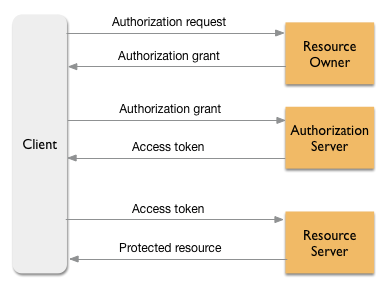
\includegraphics[width=0.85\textwidth]{images/oauth-abstract.png}
    \caption{Flusso di autorizzazione OAuth 2.0 \cite{oauth-image}}
    \label{fig:oauth-flow}
\end{figure}

\subsection{Piattaforme Fitbit e API disponibili}
Fitbit è una marca di dispositivi wearable, acquisita nel 2019 da Google \cite{fitbit}, che comprende una vasta gamma di prodotti i quali sono in grado di rilevare una grande quantità di dati.
Una volta che l'utente ha connesso il proprio dispositivo alla piattaforma Fitbit, è possibile utilizzare una serie di API che permettono di accedere a tali dati. La piattaforma Fitbit adotta lo standard OAuth 2.0 per l'autenticazione.
Tra i dati disponibili tramite le API Fitbit troviamo ad esempio:

\begin{itemize}
  \item Battito cardiaco.
  \item Calorie bruciate.
  \item Calorie assunte.
  \item Ossigenazione del sangue.
  \item Attività fisica.
  \item Sonno.
  \item Temperatura corporea.
  \item Temperatura della pelle.
  \item Attività respiratoria.
\end{itemize}

e molti altri.
Una nota da precisare è che quasi tutti i dati sono disponibili in formato intraday (ossia visibili con una frequenza che va da qualche secondo a pochi minuti). Per accedere a questo livello di dettaglio è però necessario inviare una richiesta speciale a Fitbit per ottenere l'autorizzazione necessaria alla consultazione \cite{fitbitapi}.

\subsection{Altre piattaforme e loro integrazione}

In commercio, oltre ai dispositivi Fitbit, esiste una vasta gamma di prodotti wearable per il monitoraggio dei parametri vitali con vari livelli di funzionalità: dai più economici ai più costosi. Tra questi possiamo trovare:

\begin{itemize}
  \item \textbf{Garmin Smartwatch}: dispositivi avanzati dotati di tecnologie evolute per il monitoraggio, molto adottati dagli sportivi. \cite{mysql}
  \item \textbf{Apple Watch}: orologi progettati per un'integrazione completa con l'ecosistema Apple. L'accesso ai relativi dati è più restrittivo in quanto richiede un dispositivo Apple. \cite{applewatch}
  \item \textbf{Amazfit}: dispositivi con forte competitività di prezzo rispetto alle alternative citate. \cite{amazfit}
\end{itemize}



\chapter{Analisi dei requisiti}
Per l'analisi dei requisiti (funzionali e non funzionali) è stata utilizzata la metodologia MoSCoW \cite{moscow}, la quale permette di classificare i requisiti in quattro categorie: Must have (M), Should have (S), Could have (C) e Won't have (W).

\section{Requisiti funzionali}

\subsection{Autenticazione e sicurezza - M}

\begin{itemize}
    \item Il sistema deve fornire un meccanismo sicuro di registrazione per i medici e gli operatori sanitari.
    \item Gli utenti devono potersi autenticare tramite email e password.
  \item Il sistema deve supportare l'autenticazione API tramite token JWT (JSON Web Token).
    \item Le password devono essere memorizzate con crittografia sicura (libreria Werkzeug \cite{werkzeug}).
\end{itemize}

\subsection{Gestione pazienti - M}

\begin{itemize}
    \item I medici devono poter creare nuovi record paziente con informazioni anagrafiche di base.
    \item I medici devono poter visualizzare la lista di tutti i loro pazienti.
    \item I medici devono poter visualizzare i dettagli completi di un paziente.
    \item I medici devono poter modificare le informazioni dei loro pazienti.
    \item I medici devono poter aggiungere note mediche ai record dei pazienti
\end{itemize}

\subsection{Interfaccia Utente - M}

\begin{itemize}
    \item Il sistema deve fornire una dashboard per i medici che mostri statistiche rilevanti.
    \item L'interfaccia deve essere accessibile tramite browser web standard.
    \item L'interfaccia utente deve essere responsiva per supportare diversi dispositivi.
    \item La navigazione deve essere intuitiva e coerente in tutta l'applicazione.
\end{itemize}

\subsection{API Base - M}

\begin{itemize}
    \item Il sistema deve fornire API RESTful per le operazioni CRUD sui pazienti.
    \item Le API devono supportare la ricerca e il filtraggio dei pazienti.
    \item Le API devono essere protette tramite autenticazione JWT.
    \item Le risposte API devono seguire standard coerenti e gestire gli errori in modo appropriato.
\end{itemize}

\subsection{Integrazione con Piattaforme Sanitarie - S}

\begin{itemize}
    \item Il sistema dovrebbe integrarsi con Fitbit per recuperare dati sui parametri vitali.
    \item I medici dovrebbero poter visualizzare i parametri vitali del paziente in formato grafico.
    \item Il sistema deve supportare l'autenticazione API tramite token JWT.
    \item Il sistema dovrebbe supportare l'autenticazione OAuth con le piattaforme sanitarie.
\end{itemize}

\subsection{Osservazioni sui Parametri Vitali - S}

\begin{itemize}
    \item I medici dovrebbero poter creare osservazioni sui parametri vitali dei pazienti.
    \item I medici dovrebbero poter modificare e eliminare le loro osservazioni.
    \item Il sistema dovrebbe supportare diversi tipi di parametri vitali (frequenza cardiaca, pressione sanguigna, ecc.).
    \item Le osservazioni dovrebbero essere visualizzabili in modo cronologico.
\end{itemize}

\subsection{Internazionalizzazione - S}

\begin{itemize}
    \item L'interfaccia utente dovrebbe essere disponibile in italiano e inglese.
    \item Il sistema dovrebbe consentire agli utenti di cambiare facilmente lingua.
    \item Date e numeri dovrebbero essere formattati in base alle convenzioni locali.
    \item I messaggi di errore dovrebbero essere localizzati.
\end{itemize}

\subsection{Reportistica - S}

\begin{itemize}
    \item Il sistema dovrebbe generare report base sui dati dei pazienti.
    \item I report dovrebbero essere esportabili in formati standard (PDF).
    \item I report dovrebbero essere inviabili al paziente tramite email.
    \item I medici dovrebbero poter personalizzare alcuni parametri dei report.
    \item I report generati dovrebbero essere archiviati per consultazioni future.
\end{itemize}

\subsection{Integrazione con Ulteriori Piattaforme Sanitarie - C}

\begin{itemize}
    \item Il sistema potrebbe integrarsi con Apple Health.
    \item Il sistema potrebbe integrarsi con Google Fit.
    \item Il sistema potrebbe integrarsi con Garmin Connect.
    \item Il sistema potrebbe supportare dispositivi medici Bluetooth LE.
\end{itemize}

\subsection{Collaborazione tra Medici  - C}

\begin{itemize}
    \item I medici potrebbero condividere l'accesso ai pazienti con altri medici.
    \item Il sistema potrebbe supportare commenti collaborativi sulle note mediche.
    \item I medici potrebbero ricevere notifiche quando ci sono aggiornamenti sui pazienti condivisi.
    \item Il sistema potrebbe tenere traccia di chi ha effettuato modifiche ai record.
\end{itemize}

\subsection{Autenticazione a Due Fattori  - C}

\begin{itemize}
    \item Il sistema potrebbe supportare l'autenticazione a due fattori via SMS.
    \item Il sistema potrebbe supportare l'autenticazione a due fattori via app mobile.
    \item L'utente potrebbe configurare le preferenze di sicurezza del proprio account.
    \item Il sistema potrebbe richiedere 2FA per operazioni sensibili.
\end{itemize}

\subsection{Analisi Avanzata dei Dati  - C}

\begin{itemize}
    \item Il sistema potrebbe implementare algoritmi di rilevamento anomalie nei parametri vitali.
    \item Il sistema potrebbe offrire suggerimenti basati sui trend dei dati.
    \item Il sistema potrebbe generare report comparativi tra pazienti anonimi.
    \item Il sistema potrebbe supportare la visualizzazione di correlazioni tra diversi parametri.
\end{itemize}

\subsection{Prescrizione Elettronica - W}

\begin{itemize}
    \item Il sistema non supporterà la generazione di prescrizioni elettroniche.
    \item Non ci sarà integrazione con farmacie o sistemi di prescrizione nazionali.
    \item Non sarà possibile tracciare l'aderenza ai farmaci prescritti.
    \item Non ci sarà un modulo di gestione inventario farmaci.
\end{itemize}

\subsection{Cartella Clinica Elettronica Completa  - W}

\begin{itemize}
    \item Il sistema non sostituirà una cartella clinica elettronica completa.
    \item Non ci saranno moduli per la gestione di esami di laboratorio.
    \item Non ci sarà integrazione con sistemi ospedalieri.
    \item Non ci sarà supporto per la gestione di immagini diagnostiche.
\end{itemize}

\subsection{Telemedicina  - W}

\begin{itemize}
    \item Il sistema non includerà funzionalità di videoconferenza.
    \item Non ci sarà supporto per consultazioni remote in tempo reale.
    \item Non ci saranno strumenti per la pianificazione di visite virtuali.
    \item Non ci sarà integrazione con sistemi di pagamento per visite telematiche.
\end{itemize}

\subsection{App Mobile Dedicata  - W}

\begin{itemize}
    \item Non verrà sviluppata un'app mobile dedicata nella prima fase.
    \item I pazienti non avranno accesso diretto al sistema.
    \item Non ci sarà supporto per notifiche push su dispositivi mobili.
    \item Non ci sarà funzionalità offline per l'app mobile.
\end{itemize}


\section{Requisiti non funzionali}

\subsection{Sicurezza e Privacy - M}

\begin{itemize}
    \item Tutti i dati personali dei pazienti devono essere crittografati a riposo.
    \item Deve essere implementato un sistema completo di log per gli audit di sicurezza.
\end{itemize}

\subsection{Performance  - M}

\begin{itemize}
    \item Il tempo di risposta per le operazioni di base deve essere inferiore a 2 secondi.
    \item Il sistema deve supportare almeno 1000 utenti concorrenti.
    \item Il caricamento della dashboard non deve richiedere più di 3 secondi.
    \item Il sistema deve supportare la gestione di almeno 100.000 record paziente.
\end{itemize}

\subsection{Disponibilità  - M}

\begin{itemize}
    \item Il sistema deve avere un uptime del 99,9\% durante le ore lavorative.
    \item I backup del database devono essere eseguiti quotidianamente.
\end{itemize}

\subsection{Usabilità  - M}

\begin{itemize}
    \item L'interfaccia utente deve essere utilizzabile senza formazione specifica ed essere user-friendly.
    \item I flussi di lavoro principali non devono richiedere più di 3 clic.
    \item I messaggi di errore devono essere chiari e fornire indicazioni per la risoluzione.
\end{itemize}

\subsection{Scalabilità - S}

\begin{itemize}
    \item  L'architettura dovrebbe supportare lo scaling orizzontale.
    \item Il database dovrebbe gestire efficacemente l'aumento di volume dei dati.
    \item Le prestazioni non dovrebbero degradarsi significativamente con l'aumentare degli utenti.
    \item Il sistema dovrebbe implementare tecniche di caching per migliorare la reattività.
\end{itemize}

\subsection{Manutenibilità - S}

\begin{itemize}
    \item Il codice dovrebbe seguire standard di codifica e best practice.
    \item La documentazione del codice dovrebbe essere completa e aggiornata.
    \item L'architettura dovrebbe essere modulare per facilitare gli aggiornamenti.
    \item Il sistema dovrebbe supportare aggiornamenti con tempi di inattività minimi.
\end{itemize}

\subsection{Portabilità - S}

\begin{itemize}
    \item Il sistema dovrebbe funzionare sui principali browser web (Chrome, Firefox, Edge, Safari).
    \item L'interfaccia utente dovrebbe adattarsi a diverse risoluzioni dello schermo.
    \item Il sistema dovrebbe essere containerizzato per facilitare il deployment.
    \item Il backend dovrebbe funzionare su diversi sistemi operativi server.
\end{itemize}

\subsection{Interoperabilità - S}

\begin{itemize}
    \item Le API dovrebbero seguire standard RESTful.
    \item Il sistema dovrebbe supportare almeno il formato JSON per lo scambio di dati.
    \item Il sistema dovrebbe utilizzare formati standard per date, orari e dati medici.
\end{itemize}

\subsection{Prestazioni Avanzate - C}

\begin{itemize}
    \item Il sistema potrebbe implementare tecniche di precaricamento dei dati.
    \item L'interfaccia utente potrebbe utilizzare rendering lato server per il caricamento iniziale.
    \item Il sistema potrebbe implementare la compressione delle risposte API.
    \item Il database potrebbe essere ottimizzato con indici avanzati e strategie di partizionamento.
\end{itemize}

\subsection{Monitoraggio e Analytics - C}

\begin{itemize}
    \item Il sistema potrebbe implementare dashboard di monitoraggio in tempo reale.
    \item Le metriche di prestazione potrebbero essere raccolte e analizzate.
    \item Il sistema potrebbe implementare alerting automatico per problemi prestazionali.
    \item Gli errori utente potrebbero essere tracciati per identificare problemi di usabilità
\end{itemize}

\subsection{Supporto Offline - C}

\begin{itemize}
    \item L'interfaccia utente potrebbe implementare funzionalità progressive web app.
    \item I dati critici potrebbero essere memorizzati nella cache del browser.
    \item Il sistema potrebbe supportare la sincronizzazione dei dati dopo la riconnessione.
    \item Le modifiche potrebbero essere accodate quando offline.
\end{itemize}

\subsection{Testing Automatizzato - C}

\begin{itemize}
    \item Il sistema potrebbe avere una copertura di test unitari superiore all'85\%.
    \item Il sistema potrebbe implementare test di carico programmati.
    \item Il processo di CI/CD potrebbe includere test di sicurezza automatizzati.
\end{itemize}

\subsection{Supporto Legacy - W}

\begin{itemize}
    \item Non ci sarà compatibilità con sistemi operativi obsoleti.
    \item Non verranno fornite versioni desktop standalone.
\end{itemize}

\subsection{Alta Disponibilità Geografica - W}

\begin{itemize}
    \item Il sistema non implementerà il deployment multi-regione nella prima fase.
    \item Non ci sarà failover automatico tra diversi data center.
    \item Non ci sarà ottimizzazione per utenti in regioni geografiche specifiche.
    \item Non ci sarà un sistema di content delivery network globale.
\end{itemize}

\subsection{Integrazione Enterprise Completa - W}

\begin{itemize}
    \item Non ci sarà supporto per Single Sign-On aziendale completo.
    \item Non ci sarà integrazione con sistemi ERP legacy.
    \item Non ci saranno connettori personalizzati per ogni sistema clinico.
\end{itemize}

\subsection{Conformità Internazionale Completa - W}

\begin{itemize}
    \item Il sistema non sarà inizialmente certificato per standard internazionali come HIPAA.
    \item Non ci sarà supporto completo per tutti i requisiti normativi regionali.
    \item Non ci saranno localizzazioni complete per tutti i paesi.
    \item Non ci sarà certificazione FDA come dispositivo medico.

\end{itemize}

\section{Casi d'uso}
\subsection{Attori principali}
I principali attori del sistema risultano essere i medici e gli operatori sanitari, i quali si interfacciano con il sistema per la gestione dei pazienti e dei dati clinici.
I pazienti non hanno accesso diretto al sistema, ma possono comunque ricevere via email i report generati e sono necessari nel flusso di autenticazione necessario per concedere l'accesso dei proprio dati al sistema.
\subsection{Gestione dei pazienti}
I medici e gli operatori sanitari possono:
\begin{itemize}
    \item Visualizzare i pazienti.
    \item Creare nuovi pazienti.
  \item Importare pazienti tramite UUID (Universally Unique Identifier).
    \item Visualizzare i dettagli di un paziente.
    \item Modificare i dettagli di un paziente.
    \item Eliminare un paziente(dissociandolo dal proprio account).
\end{itemize}
\subsection{Gestione dell'account}
I medici e gli operatori sanitari possono:
\begin{itemize}
    \item Registrare un nuovo account.
    \item Eseguire il login.
    \item Eseguire il logout.
\end{itemize}
\subsection{Visualizzazione dei parametri vitali}
I medici e gli operatori sanitari possono:
\begin{itemize}
    \item Visualizzare grafici dei parametri vitali.
    \item Visualizzare i parametri vitali in formato di tabelle.
    \item Selezionare un livello di dettaglio per la visualizzazione dei dati (1g, 7g, 30g, 90g).
\end{itemize}
\subsection{Gestione note}
I medici e gli operatori sanitari possono:
\begin{itemize}
    \item Creare nuove note cliniche.
    \item Visualizzare note esistenti.
    \item Eliminare note(solo quelle create da loro).
    \item Visualizzare i dettagli di un paziente.
    \item Modificare i dettagli di un paziente.
    \item Eliminare un paziente.
\end{itemize}
\subsection{Gestione report}
I medici e gli operatori sanitari possono:
\begin{itemize}
    \item Generare report specifici relativi ad un parametro vitale.
    \item Generare un report generale relativo a tutti i parametri vitali.
    \item Selezionare gli elementi(note, osservazioni, grafici) da includere nel report.
    \item Scaricare il report in formato PDF.
    \item Inviare una copia per email al paziente del report in formato PDF.
\end{itemize}
\subsection{Integrazione con piattaforme sanitarie}
I pazienti possono:
\begin{itemize}
    \item Autorizzare la connessione del proprio account alla piattaforma.
\end{itemize}
La piattaforma su cui sono salvati i dati può:
\begin{itemize}
    \item Revocare l'autorizzazione di accesso al sistema.
\end{itemize}
I medici e gli operatori sanitari possono:
\begin{itemize}
    \item Generare un link valido 24h per permettere all'utente di fornire l'accesso da parte della piattaforma ai suoi dati.
  \item Rimuovere il collegamento alla piattaforma su cui sono salvati i dati.
\end{itemize}
\subsection{Gestione delle osservazioni cliniche}
I medici e gli operatori sanitari possono:
\begin{itemize}
    \item Creare un'osservazione clinica relativa ad un parametro vitale e ad un periodo temporale specifico.
    \item Visualizzare le note esistenti per ciascun paziente.
    \item Eliminare un'osservazione clinica(solo quelle create da loro).
\end{itemize}



\section{User stories e scenari comuni principali}
\subsection{Registrazione e accesso}
\begin{itemize}
  \item Accesso alla piattaforma via browser.
    \item Si presentano due opzioni: registrazione e login.
    \item Per registrarsi l'utente clicca sul collegamento "Nuovo medico? Registrati Qui"(La lingua effettiva dipende dalla localizzazione selezionata).
  \item L'utente, seguendo le richieste specificate nella pagina, compila i campi con i propri dati, facendo attenzione a rispettare i requisiti di sicurezza della password.
    \item Se tutto è stato inserito correttamente, non esistono altri account nel sistema con la stessa email e il sistema non ha restituito errori, dopo aver premuto il pulsante "Crea Account" l'utente viene registrato e reindirizzato alla pagina di login.
    \item L'utente può accedere al sistema inserendo la propria email e password.
    \item L'utente, se i dati sono corretti e se il sistema non ha restituito errori, dopo aver premuto il pulsante "Accedi" viene reindirizzato alla Dashboard del sistema.
\end{itemize}
\subsection{Importazione e gestione pazienti}
\begin{itemize}
  \item Dalla Dashboard iniziale avvia la gestione pazienti.
    \item Decide di aggiungere un paziente: clicca sulla shortcut nella Dashboard "Nuovo Paziente" nel Menù Azioni rapide(oppure va nella pagina "Visualizza tutti i pazienti" e clicca sul pulsante "Aggiungi nuovo paziente").
    \item Nel form che si apre, l'utente compila i campi obbligatori richiesti e, se desidera, quelli opzionali.
    \item Dopo aver compilato il form, se i dati inseriti sono validi e se il sistema non ha restituito errori, dopo aver cliccato il pulsante "Salva Paziente" verrà creato un nuovo account.
    \item Dalla schermata "Visualizza tutti i pazienti" l'utente può importare un paziente esistente tramite UUID cliccando sul pulsante "Importa Paziente tramite UUID".
    \item Nel modale che si aprirà, l'utente inserirà il codice di associazione richiesto.
    \item Se il codice di associazione inserito è valido e associato ad un account paziente esistente (e se il sistema non ha restituito errori), dopo il click sul pulsante "Importa Paziente" il paziente verrà aggiunto alla lista dei pazienti seguiti dall'operatore.
\end{itemize}
\subsection{Collegamento dispositivi wearable}
\begin{itemize}
  \item Punto di partenza: Dashboard.
    \item Decide di collegare un dispositivo wearable al profilo di un paziente: clicca sul pulsante "Visualizza tutti i pazienti" e, sulla lista dei pazienti, clicca sul pulsante Azione "Visualizza i parametri vitali".
    \item Nella pagina che si trova davanti, l'utente clicca sul pulsante "Health Sync".
    \item Viene aperto un modale che mostra un QR Code (per permettere ad un paziente in visita al medico di collegarsi scansionandolo) ed un link testuale che può essere condiviso con il paziente tramite email o messaggio.
    \item Il paziente, una volta ricevuto il link, cliccando su di esso viene reindirizzato alla pagina di autorizzazione all'accesso ai propri dati da parte del sistema, la quale può essere raggiungibile per 24h (o comunque fino a che la procedura di autorizzazione non sarà riuscita). Se il link non dovesse essere più valido il paziente verrà informato di questo.
  \item Il paziente clicca sul servizio relativo al dispositivo che possiede (inizialmente saranno supportati solo i dispositivi Fitbit).
    \item Si apre la pagina di login della piattaforma scelta, la quale dopo aver effettuato l'accesso chiede all'utente di autorizzare una certa serie di permessi al sistema richiedente.
    \item Una volta concessi, l'utente viene reindirizzato alla pagina dei servizi disponibili e gli viene comunicato l'esito dell'operazione(fallita o riuscita).
    \item Il medico è ora collegato al dispositivo del paziente e può visualizzare i dati relativi ai parametri vitali nella schermata in cui ha cliccato "Health Sync".
\end{itemize}
\subsection{Visualizzazione e interpretazione dei dati}
\begin{itemize}
  \item Apertura dalla Dashboard.
    \item Clicca su "Visualizza tutti i pazienti" e clicca sull'azione "Visualizza Paziente".
  \item Qui il medico può interagire con le note relative al paziente, oltre che a visualizzare i relativi dati di registrazione.
    \item Clicca sul pulsante "Visualizza i parametri vitali" e si apre la pagina con i dati relativi al parametri vitali del paziente.
    \item Il medico, dopo che è stato effettuato il collegamento al dispositivo wearable, può visualizzare i dati relativi ai parametri vitali in formato tabellare o grafico.
    \item Il medico può decidere il livello di dettaglio di visualizzazione dei dati andando a cliccare sul pulsante relativo al periodo scelto(1g, 7g, 30g, 90g).
    \item Il medico può cambiare il parametro vitale visualizzato cliccando sulla voce relativa al parametro vitale desiderato.
\end{itemize}

\subsection{Generazione e invio report}
\begin{itemize}
  \item Avvio dalla Dashboard.
    \item Clicca su "Visualizza tutti i pazienti" e clicca sull'azione "Visualizza Parametri Vitali".
    \item Nella schermata che si apre, il medico visualizza i dati relativi ai parametri vitali del paziente.
  \item Nella sezione "Reports" il medico può scegliere di aprire la pagina di generazione del report relativa a tutti i parametri o ad un singolo parametro vitale specifico.
    \item Se si sceglie su un parametro vitale specifico, la pagina verrà aperta con selezionato in automatico il grafico da includere nel report relativo al parametro vitale che era visualizzo nella pagina precedente(e con lo stesso livello di dettaglio).
    \item Se si sceglie su "Report Completo", la pagina verrà aperta con selezionati in automatico tutti i grafici relativi ai parametri vitali presenti(con il livello di dettaglio che era selezionato).
    \item In qualsiasi caso è possibile aggiungere o rimuovere parametri vitali e/o grafici. Inoltre è possibile aggiungere o rimuovere note cliniche e osservazioni cliniche.
    \item Il medico può inserire un messaggio opzionale riepilogativo con eventuali suggerimenti per il paziente.
    \item Il medico può selezionare di inoltrare una copia del report al paziente via email(solo se questa è stata inserita nel campo opzionale del paziente al momento della registrazione).
  \item Il medico clicca su "Genera Report PDF" e una copia PDF del report verrà scaricata sul dispositivo.
    \item Se selezionata l'opzione di invio email, il sistema invierà una copia del report anche al paziente tramite email.
\end{itemize}

\subsection{Visualizzazione degli audit}
\begin{itemize}
  \item Accesso dalla Dashboard.
    \item Clicca sul pulsante "Visualizza i Log delle Attività" e sistema si apre la pagina con gli audit.
    \item Il medico visualizza una pagina con tutte le operazioni eseguite sugli utenti che esso segue (generati o importati) organizzate per "Azione" ed "Entità".
    \item Il medico può filtrare i dati per utente, Data(inizio e fine), tipo di azione, tipo di entità, paziente.
    \item Il medico può visualizzare dei grafici riepilogativi delle azioni eseguite in fondo alla pagina.
\end{itemize}

\subsection{Modifica dati personali}
\begin{itemize}
  \item Ingresso dalla Dashboard.
    \item Clicca sul pulsante in alto a destra col proprio nome.
    \item Nella tendina che si apre clicca su "Profilo".
    \item Si apre una pagina con i suoi dati personali.
    \item Per modificare i propri dati, il medico aggiorna i campi contenenti i vecchi dati con quelli nuovi e, verificando che questi soddisfino la validazione, clicca su "Aggiorna Profilo" (per i dati normali) o "Aggiorna passato" (per la password).
    \item Se i dati inseriti sono validi e il sistema non ha restituito errori, il medico riceve un messaggio che lo informa dell'avvenuto aggiornamento dei suoi dati.
\end{itemize}

\chapter{Progettazione}
\section{Architettura del sistema}
\subsection{Architettura generale e componenti principali}
VitaLink è strutturata come un'applicazione web progettata per essere altamente scalabile e modulabile. Essa utilizza il framework Flask (Python) per il backend, Bootstrap per il frontend e PostgreSQL come database relazionale (ma è possibile sostituirlo facilmente con un DBMS analogamente relazionale).
La piattaforma è progettata per essere inizialmente accessibile solo tramite browser web, ma sono state inserite anche delle API per permettere l'integrazione futura con possibili app mobile o altri sistemi esterni.
\subsection{Modularità e separazione delle responsabilità}
La piattaforma è divisa in 15 moduli principali, ai quali vanno ad affiancarsi due moduli di supporto per la gestione delle migrazioni e per la compilazione delle traduzioni al momento dell'istanziazione di un un container.
Vi sono poi le directory dei file static e dei template per quanto concerne il frontend, e la directory delle traduzioni per contenere le varie localizzazioni seguendo lo standard di Flask Babel.
Infine nella root del progetto è presente la cartella dei test. La cartella contiene inoltre un file di configurazione per la creazione di un ambiente e la fornitura di funzioni per la gestione dei test.
\vspace{1em}
\dirtree{%
    .1 \textbf{VitaLink}/.
    .2 docs/ \ldots{} (documentazione).
    .2 app/.
    .3 static/.
    .4 css/.
    .5 custom.css (stile dell'applicazione).
    .5 health\_connect.css (stile pagina collegamento dispositivi).
    .4 img/.
    .5 fitbit-logo.png (logo Fitbit).
    .5 apple-health-logo.png (logo Apple Health).
    .5 health-connect-logo.png (logo Google Health Connect).
    .4 js/.
    .5 health\_platforms.js.
    .5 main.js.
    .5 observations.js.
    .5 patients.js.
    .5 specific\_report.js.
    .5 translations.js.
    .5 vital\_charts.js.
    .5 vitals.js.
    .3 templates/.
    .4 audit\_logs.html.
    .4 base-no-session.html.
    .4 base.html.
    .4 dashboard.html.
    .4 health\_connect\_result.html.
    .4 health\_connect.html.
    .4 login.html.
    .4 patient\_detail.html.
    .4 patients.html.
    .4 profile.html.
    .4 register.html.
    .4 specific\_report\_form.html.
    .4 vitals.html.
    .3 translations/.
    .4 babel.cfg (configurazione Babel).
    .4 messages.pot (template traduzioni).
    .4 it/ (traduzioni in italiano).
    .3 \_\_init\_\_.py.
    .3 app.py (configurazione applicazione e database).
    .3 audit.py (gestione log di audit).
    .3 auth.py (definizione autorizzazioni).
    .3 compile\_translations.py (compilazione traduzioni).
    .3 email\_utils.py (integrazione API invio email).
    .3 health\_platforms\_config.py (definizione API piattaforme sanitarie).
    .3 health\_platforms.py (recupero dati dalle API).
    .3 language.py (gestione lingue).
    .3 main.py (punto di ingresso dell'applicazione).
    .3 migrate.py (gestione migrazione database).
    .3 models.py (definizione modelli database).
    .3 observations.py (gestione osservazioni cliniche).
    .3 reports.py (generazione report).
    .3 utils.py (funzioni di utilità).
    .3 views.py (viste web).
    .3 api.py (endpoint API RESTful).
    .2 tests/ (test unitari e di integrazione).
    .2 Dockerfile (configurazione immagine Docker).
    .2 docker-compose.yml (configurazione container Docker).
    .2 docker-entrypoint.sh (script avvio container).
    .2 .env.example (struttura variabili d'ambiente).
    .2 .env (configurazione locale).
    .2 db\_migrate.yml (migrazione automatica in Docker).
    .2 pyproject.toml (dipendenze e configurazione test).
    .2 .dockerignore (esclusioni per Docker).
    .2 .gitignore (esclusioni per Git).
}
\subsection{Flusso dei dati e interazioni tra componenti}
Il frontend interagisce con il backend mediante richieste HTTP alle API RESTful della piattaforma, ricevendo risposte in formato JSON.
Queste API sono protette mediante autenticazione JWT o sessioni, facendo in modo che solo gli utenti autorizzati possano accedere ai dati. Il backend, implementato con Flask, gestisce tali richieste attraverso moduli specializzati come \texttt{auth.py} per l'autenticazione, \texttt{views.py} per le viste web e \texttt{api.py} per gli endpoint REST.
I dati rimangono immagazzinati nel database PostgreSQL, accessibile tramite l'ORM SQLAlchemy \cite{sqlalchemy} che astrae le interazioni a livello SQL.
Una componente chiave per l'obiettivo della piattaforma è il modulo \texttt{health\_platforms.py} che gestisce l'integrazione con servizi esterni come Fitbit mediante OAuth 2.0: quando un paziente autorizza l'accesso ai propri dati, il sistema riceve token di accesso e refresh che vengono memorizzati e associati al profilo dell'utente interessato.
Successivamente, il sistema può recuperare i dati sanitari chiamando le API esterne, elaborarli secondo le regole in \texttt{health\_platforms\_config.py} e memorizzarli temporaneamente nella cache per ottimizzare le prestazioni e ridurre le chiamate API (mitigando la possibilità di incorrere in blocchi).

\section{Design pattern}
Tra i pattern architetturali adottati nel progetto possiamo citare i più rilevanti.
\subsection{Pattern architetturali}
\begin{itemize}
    \item MVC (Model-View-Controller): separa la logica di business dalla presentazione, dell'interazione con la base di dati e della logica di controllo.
    \item Function Organization Pattern : ogni modulo è organizzato in funzioni, ciascuna delle quali ha una responsabilità specifica e coerente con la natura del modulo stesso.
\end{itemize}
\subsection{Pattern di progettazione}
\begin{itemize}
    \item Factory Pattern: utilizzato per creare oggetti in una superclasse, permettendo alle sottoclassi di alterare il tipo di oggetto creato.
    \item Strategy Pattern: permette di definire una famiglia di algoritmi incapsulati in classi separate.
    \item Decorator Pattern: permette di aggiungere responsabilità aggiuntive ad un oggetto senza modificarne la struttura.
\end{itemize}
\section{Modello dei dati}
Per il modello dei dati è stato scelto un approccio relazionale in quanto non vi è una particolare necessità di un modello noSQL, essendo i dati sanitari di tipo strutturato e relazionabile.
\subsection{Entità principali e relazioni - Schema ER}
\begin{figure}[H]
    \centering
    \includegraphics[width=0.85\textwidth]{images/DataModel.png}
    \caption{Schema ER completo del database}
    \label{fig:Schema-ER}
\end{figure}
\subsection{Enumerazioni e tipi di dati}
È stato scelto di utilizzare i tipi di dati standard di PostgreSQL per la definizione dei campi del database, in quanto sono sufficienti a soddisfare gli obiettivi perseguiti.
Sono presenti 4 Enum nel database utilizzati per casi specifici per garantire l'integrità dei dati e limitare i valori possibili ad un insieme predefinito di costanti.
\begin{itemize}
    \item Tipi di parametri vitali
    \item Tipo di piattaforma sanitaria
    \item Tipo di attività per l'audit
    \item Tipo di entità per l'audit
\end{itemize}
\section{Architettura del database}
È stato scelto PostgreSQL come DBMS relazionale in quanto risulta essere uno dei più diffusi e supportati dalle piattaforme per il deployment.
Non è comunque esclusa la possibilità di poter riconfigurare il sistema per l'utilizzo di un altro DBMS relazionale, come ad esempio MySQL o Microsoft SQL Server.
\subsection{Strategia di migrazione}
Sono presenti 2 file nel progetto per le migrazioni del database:
Lo script db\_migrate.sh è un file che viene utilizzato nelle situazioni di deployment (o comunque di istanziazione del container) per la creazione del database e delle tabelle necessarie e l'aggiornamento della struttura del database.
Lo script migrate.py è un file che viene utilizzato per la migrazione del database in fase di sviluppo locale, per la creazione delle tabelle e per l'aggiornamento della struttura del database.
Da notare che che per lo sviluppo locale si rende necessaria la creazione del database dall'istanza di PostgreSQL locale, mentre per il deployment è sufficiente, nel caso in cui non si sfrutti un database interno al container, specificare il nome del database nel file .env.
Nel caso invece in cui in fase di deployment si decida di utilizzare un database esterno al container, valgono le stesse considerazioni fatte per lo sviluppo locale, ossia si rende necessaria la creazione del database sul provider del servizio database scelto.
\section{Interfaccia utente}
\subsection{Design responsivo}
L'interfaccia utente è stata progettata per essere quanto più intuitiva e semplice possibile seguendo un approccio per formulare un design responsivo, utile per facilitare la consultazione dei dati sanitari su un'ampia gamma di dispositivi.
La decisione di utilizzare Bootstrap per il frontend ha permesso di ridurre la mole di lavoro necessaria per questo tipo di task, consentendo di focalizzare gli sforzi di sviluppo su parti più cruciali del sistema.
Le pagine sono state sviluppate con un design moderno e intuitivo, adatto per l'uso anche da parte di personale sanitario non addestrato all'uso dello strumento.
Ciascuna pagina presenta un menù accessibile nella parte superiore dello schermo che permette un accesso rapido a:
\begin{itemize}
    \item Dashboard
    \item Visualizza tutti i pazienti
    \item Visualizza i log di audit
    \item Menù a tendina con il nome dell'utente
    \item Selezione della lingua
          \begin{itemize}
              \item Profilo
              \item Logout
          \end{itemize}
\end{itemize}
Nelle pagine di generazione dei report e di concessione dell'autorizzazione di accesso ai dati dei parametri vitali (per i pazienti) questo menù è stato rimosso per motivi di design in quanto queste pagine non sono state progettate come routes accessibili permanentemente, ma solo temporaneamente per determinate task.
\subsection{Componenti UI per la visualizzazione dei dati sanitari}
Per la visualizzazione dei dati sanitari sono stati utilizzati grafici generati con la libreria Chart.js \cite{chartjs}, che permette di generare grafici personalizzabili e interattivi con un design accattivante.
Inoltre i dati sanitari sono accessibili anche in formato tabellare, utile soprattutto per quei dati la cui rappresentazione grafica risulta poco utile, come ad esempio il cibo assunto o diari dell'utente.
\section{API e integrazione con sistemi esterni}


\subsection{RESTful API design}
L'architettura di VitaLink è stata progettata includendo i principi del paradigma REST (Representational State Transfer) \cite{rest}, ossia un insieme di vincoli e proprietà basati sul protocollo HTTP per la creazione di servizi web. L'implementazione di un'API RESTful ha permesso di ottenere un'interfaccia standardizzata, scalabile e facilmente integrabile con sistemi esterni e possibili applicazioni di terze parti.

\subsubsection{Principi di progettazione}
Nella progettazione delle API di VitaLink sono stati seguiti i seguenti principi fondamentali REST:

\begin{itemize}
    \item \textbf{Architettura client-server}: anche se frontend e backend sono inclusi nella stessa immagine Docker, mantengono una separazione logica e comunicano tramite richieste HTTP, rispettando il principio dell'architettura client-server.
    \item \textbf{Statelessness}: ogni richiesta dal client al server contiene tutte le informazioni necessarie per capire e processare la richiesta, senza dipendere da contesti memorizzati sul server.
    \item \textbf{Interfaccia uniforme}: tutte le risorse sono accessibili attraverso un'interfaccia standardizzata che utilizza i metodi HTTP (GET, POST, PUT, DELETE).
    \item \textbf{Sistema a livelli}: l'architettura è organizzata in livelli, con ogni componente che svolge un ruolo specifico.
    \item \textbf{Risorse identificabili}: ogni risorsa è identificata univocamente attraverso URI (Uniform Resource Identifier).
\end{itemize}

\subsubsection{Struttura delle risorse}
L'API è strutturata attorno a risorse chiaramente identificate. Tra le risorse possiamo trovare:

\begin{itemize}
    \item \texttt{/patients}: gestione dei pazienti.
    \item \texttt{/patients/<uuid>/vitals}: parametri vitali di un paziente specifico.
  \item \texttt{/patients/<uuid>/notes}: note mediche associate ad un paziente.
    \item \texttt{/observations}: osservazioni mediche.
\end{itemize}

\subsubsection{Metodi HTTP semantici}
I metodi HTTP sono utilizzati per le operazioni CRUD (Create, Read, Update, Delete):

\begin{itemize}
    \item \texttt{GET}: recupero di risorse (es. lista pazienti, parametri vitali).
    \item \texttt{POST}: creazione di nuove risorse (es. aggiunta di una nota medica).
    \item \texttt{PUT}: aggiornamento di risorse esistenti (es. modifica di un'osservazione).
    \item \texttt{DELETE}: rimozione di risorse (es. eliminazione di una nota).
\end{itemize}

\subsubsection{Rappresentazione delle risorse}
Le risorse sono rappresentate in formato JSON \cite{json}.
Un esempio di rappresentazione per una richiesta di parametri vitali:

\begin{verbatim}
{
    "heart_rate": [
        {
            "timestamp": "2023-05-01T14:30:00Z",
            "value": 72,
            "unit": "bpm"
        },
        ...
    ]
}
\end{verbatim}

\subsubsection{Codici di stato HTTP}
Le API utilizzano codici di stato HTTP standard per fornire il risultato delle operazioni:

\begin{itemize}
    \item \textbf{200 OK}: operazione completata con successo (GET, PUT, DELETE)
    \item \textbf{201 Created}: risorsa creata con successo (POST)
    \item \textbf{400 Bad Request}: richiesta non valida (parametri mancanti o errati)
    \item \textbf{401 Unauthorized}: autenticazione mancante o non valida
    \item \textbf{403 Forbidden}: accesso non autorizzato alla risorsa richiesta
    \item \textbf{404 Not Found}: risorsa non trovata
    \item \textbf{500 Internal Server Error}: errore del server
\end{itemize}

\subsubsection{Autenticazione e autorizzazione}
L'accesso alle API è protetto tramite autenticazione JWT (JSON Web Token) per garantire:

\begin{itemize}
    \item \textbf{Sicurezza}: comunicazioni crittografate con il server
    \item \textbf{Statelessness}: ogni richiesta contiene tutte le informazioni necessarie per l'autenticazione
    \item \textbf{Granularità dei permessi}: verifica che il medico abbia accesso al paziente richiesto
\end{itemize}

\subsubsection{Documentazione delle API}
Le API sono completamente documentate con docstring Python dettagliate (compilabili con il pacchetto mkdocs) che specificano:

\begin{itemize}
    \item Scopo dell'endpoint
    \item Parametri di input richiesti e opzionali
    \item Formato della risposta
    \item Possibili codici di stato e loro significato
    \item Esempi di utilizzo
\end{itemize}

\subsubsection{Gestione degli errori}
È stato implementato un sistema di gestione degli errori che fornisce messaggi di errore chiari e dettagliati in formato JSON. Ad esempio:

\begin{verbatim}
{
    "error": "Patient not found",
    "details": "No patient with the provided UUID exists"
}
\end{verbatim}

\subsection{Integrazione OAuth con Fitbit}
Per l'integrazione con i dispositivi Fitbit, l'applicazione utilizza il flusso di autorizzazione OAuth 2.0.
Ciò consente agli utenti di autorizzare l'accesso ai propri dati sanitari senza condividere le proprie credenziali.
Una volta che l'utente ha autorizzato l'accesso, l'applicazione riceve un token di accesso che può essere usato per effettuare richieste alle API di Fitbit per recuperare i dati dei parametri vitali. Viene inoltre fornito un token refresh per ottenere un nuovo token di accesso una volta che quello precedente è scaduto (di base i token di accesso per fitbit scadono dopo 8 ore).

\subsection{Sistema di caching temporaneo}
Per ottimizzare le prestazioni e ridurre il numero di chiamate API con possibile conseguente superamento del rate limit specifico di una piattaforma, è stato implementato un sistema di caching temporaneo. Questo sistema memorizza nella cache i dati recentemente recuperati, in modo da poterli riutilizzare senza dover effettuare una nuova richiesta alle API. Questo approccio aiuta a rispettare i limiti di rate imposti da alcune API.
Il sistema di caching è implementato utilizzando una struttura dati principale chiamata \texttt{vitals\_cache} che memorizza i dati dei parametri vitali recuperati dalle API.
Ogni voce della cache è indicizzata con una chiave univoca composta come:
\begin{lstlisting}[basicstyle=\small\ttfamily, breaklines=true]
cache_key = f"{patient.id}_{normalized_data_type}_{start_date}_{end_date}"
\end{lstlisting}

Il sistema implementa un meccanismo di time-to-live (TTL) configurabile attraverso il parametro \texttt{text\_duration}, impostato a 300 secondi di default. Quando viene richiesto un dato l'algoritmo:
\begin{itemize}
    \item Verifica se esiste una chiave corrispondente nella cache
    \item Se esiste, controlla la validità temporale della cache tramite il comando:
          \begin{lstlisting}[basicstyle=\small\ttfamily, breaklines=true]
    cache_age = (datetime.utcnow() - cache_time).total_seconds()
    if cache_age < cache_duration:
        Cache valida, usa i dati memorizzati
    \end{lstlisting}
    \item Se la cache è scaduta o non esiste, esegue la chiamata API alla piattaforma esterna e aggiorna la cache con i nuovi dati ottenuti

\end{itemize}

\subsection{Estendibilità per future piattaforme}
L'architettura delle API è stata progettata tenendo in considerazione l'estensione futura dei servizi offerti. Ciò significa che, in futuro, sarà possibile integrare facilmente nuove piattaforme e dispositivi semplicemente aggiungendo nuove implementazioni dei servizi e configurando le relative API, senza dover apportare modifiche all'architettura.



\chapter{Implementazione}
\section{Stack tecnologico}
\subsection{Backend: Python e Flask}
Il backend della piattaforma è stato sviluppato mediante l'uso di Python e del framework Flask relativo. Python è un linguaggio di programmazione molto flessibile e supportato da una vasta gamma di librerie. La conoscenza pregressa e l'utilizzo di Flask sono state le ragioni più rilevanti per la scelta del framework.
\subsection{ORM: SQLAlchemy}
Per la gestione delle interazioni con il database, è stato utilizzato SQLAlchemy, un ORM (Object-Relational Mapping) \cite{orm} per Python.
Esso permette di interagire con il database utilizzando oggetti Python invece di scrivere direttamente query SQL, semplificando così lo sviluppo e la manutenzione del codice.


\subsection{Frontend: HTML5, CSS3, JavaScript, Bootstrap}
Il frontend dell'applicazione è stato realizzato utilizzando tecnologie web standard come HTML5, CSS3 e JavaScript. L'utilizzo del framework Bootstrap ha semplificato e velocizzato lo sviluppo di un'interfaccia utente responsive e moderna.
Anche le funzioni JavaScript sono state implementate in moduli separati per garantire una migliore organizzazione del codice e suddivisione delle responsabilità.
Ciascuna funzione è stata documentata con docstring dettagliate.

\subsection{Containerizzazione: Docker}
L'utilizzo di Docker ha permesso di creare un ambiente di sviluppo e produzione isolato facilmente replicabile.
Un file Dockerfile è stato configurato per definire l'immagine del container, mentre un file docker-compose.yml è stato utilizzato per gestire il container nello sviluppo locale
\begin{lstlisting}[basicstyle=\small\ttfamily, breaklines=true, caption={Dockerfile}]
FROM python:3.11-slim
WORKDIR /app

RUN apt-get update && apt-get install -y --no-install-recommends \
    gcc libpq-dev postgresql-client iproute2 net-tools curl dos2unix \
    && rm -rf /var/lib/apt/lists/*

COPY . /app/

RUN pip install --no-cache-dir --upgrade pip \
 && pip install --no-cache-dir .

RUN mkdir -p /app/uploads && chmod 777 /app/uploads

RUN dos2unix /app/docker-entrypoint.sh \
 && chmod +x /app/docker-entrypoint.sh \
 && dos2unix /app/db_migrate.sh \
 && chmod +x /app/db_migrate.sh

EXPOSE $PORT

ENTRYPOINT ["/app/docker-entrypoint.sh"]
CMD ["sh", "-c", "/app/db_migrate.sh && gunicorn --bind $HOST:$PORT --workers 3 --access-logfile - --error-logfile - --log-level $(echo ${LOG_LEVEL} | tr '[:upper:]' '[:lower:]') $FLASK_APP"]
\end{lstlisting}

\begin{lstlisting}[basicstyle=\small\ttfamily, breaklines=true, caption={docker-compose.yml}]
services:
  web:
    build:
      context: .
      dockerfile: Dockerfile
    ports: ["${PORT}:${PORT}"]
    depends_on: [db]
    env_file: .env  
    volumes:
      - ./uploads:/app/uploads
    healthcheck:
      test: ["CMD", "curl", "-f", "http://${HOST}:${PORT}/"]
      interval: 30s
      timeout: 10s
      retries: 3
      start_period: 40s

  db:
    image: postgres:15-alpine
    env_file: .env
    environment:
      POSTGRES_USER:  ${PGUSER}
      POSTGRES_PASSWORD: ${PGPASSWORD}
      POSTGRES_DB: ${PGDATABASE}
    volumes:
      - postgres_data:/var/lib/postgresql/data
    ports: ["${PGPORT}:${PGPORT}"]
    healthcheck:
      test: ["CMD-SHELL", "pg_isready -U ${PGUSER}"]
      interval: 10s
      timeout: 5s
      retries: 5
      start_period: 10s

volumes:
  postgres_data:
\end{lstlisting}
Si può notare come nel file Dockerfile vengono chiamati gli script di inizializzazione db\_migrate.sh e docker-entrypoint.sh.
Il loro utilizzo risulta fondamentale per la corretta configurazione del container e per la corretta inizializzazione del database.
Non vengono invece chiamati nelle fasi di sviluppo locale.

\subsection{Variabili d'ambiente e configurazione}
L'uso di variabili d'ambiente permette una configurazione personalizzata e flessibile dell'applicazione in contesti differenti.
Di seguito è possibile trovare 3 esempi di configurazione delle variabili d'ambiente per 3 situazioni differenti:
\begin{itemize}
    \item \textbf{.env.tests per tests:}
          \begin{itemize}
              \item \textbf{Connessione al database:}
                    \begin{itemize}
                        \item \texttt{DATABASE\_URL}: sqlite:///test\_healthcare.db
                    \end{itemize}

              \item \textbf{Configurazione dell'applicazione:}
                    \begin{itemize}
                        \item \texttt{FLASK\_APP}:app:app
                        \item \texttt{SESSION\_SECRET}:chiave segreta per la firma delle sessioni utente
                        \item \texttt{JWT\_SECRET\_KEY}:chiave per la firma dei token JWT
                        \item \texttt{HOST}, \texttt{PORT}:0.0.0.0
                        \item \texttt{DEBUG}:<true/false>
                        \item \texttt{PORT}:<port>
                        \item \texttt{LOG\_LEVEL}:<NOTSET/DEBUG/INFO/WARN/ERROR/CRITICAL>
                    \end{itemize}

              \item \textbf{Ambiente di esecuzione:}
                    \begin{itemize}
                        \item \texttt{CLOUD\_RUN\_ENVIRONMENT}:false
                    \end{itemize}
          \end{itemize}

    \item \textbf{.env per sviluppo locale:}
          \begin{itemize}
              \item \textbf{Connessione al database:}
                    \begin{itemize}
                        \item \texttt{PGHOST}:<db\_host>
                        \item \texttt{PGPORT}:<port>
                        \item \texttt{PGUSER}:<user>
                        \item \texttt{PGPASSWORD}:<password>
                        \item \texttt{PGDATABASE}:<db\_name>
                        \item \texttt{DATABASE\_URL}:sqlite:///test\_healthcare.db
                    \end{itemize}

              \item \textbf{Configurazione dell'applicazione:}
                    \begin{itemize}
                        \item \texttt{FLASK\_APP}:app:app
                        \item \texttt{SESSION\_SECRET}:chiave segreta per la firma delle sessioni utente
                        \item \texttt{JWT\_SECRET\_KEY}:chiave per la firma dei token JWT
                        \item \texttt{HOST}, \texttt{PORT}:0.0.0.0
                        \item \texttt{DEBUG}:<true/false>
                        \item \texttt{LOG\_LEVEL}:<NOTSET/DEBUG/INFO/WARN/ERROR/CRITICAL>
                        \item \texttt{PORT}:<port>
                    \end{itemize}
              \item \textbf{Configurazione delle API:}
                    \begin{itemize}
                        \item \texttt{FITBIT\_CLIENT\_ID}:<fitbit\_id>
                        \item \texttt{FITBIT\_CLIENT\_SECRET}:<fitbit\_secret>
                        \item \texttt{FITBIT\_REDIRECT\_URI}:<fitbit\_callback\_uri>
                        \item \texttt{MJ\_APIKEY}:<api\_key>
                        \item \texttt{MJ\_APIKEY\_SECRET}:<secret\_key>
                        \item \texttt{EMAIL\_SENDER}:<email\_sender>
                    \end{itemize}
              \item \textbf{Ambiente di esecuzione:}
                    \begin{itemize}
                        \item \texttt{CLOUD\_RUN\_ENVIRONMENT}:false
                    \end{itemize}
          \end{itemize}

    \item \textbf{.env per deploy cloud:}

          \begin{itemize}
              \item \textbf{Connessione al database:}
                    \begin{itemize}
                        \item \texttt{PGUSER}:<user>
                        \item \texttt{PGPASSWORD}:<password>
                        \item \texttt{PGDATABASE}:<db\_name>
                        \item \texttt{INSTANCE\_UNIX\_SOCKET}:<connection\_name>
                    \end{itemize}

              \item \textbf{Configurazione dell'applicazione:}
                    \begin{itemize}
                        \item \texttt{FLASK\_APP}:app:app
                        \item \texttt{SESSION\_SECRET}:chiave segreta per la firma delle sessioni utente
                        \item \texttt{JWT\_SECRET\_KEY}:chiave per la firma dei token JWT
                        \item \texttt{HOST}, \texttt{PORT}:0.0.0.0
                        \item \texttt{DEBUG}:<true/false>
                        \item \texttt{LOG\_LEVEL}:<NOTSET/DEBUG/INFO/WARN/ERROR/CRITICAL>
                        \item \texttt{PORT}:<port>
                    \end{itemize}
              \item \textbf{Configurazione delle API:}
                    \begin{itemize}
                        \item FITBIT\_CLIENT\_ID:<fitbit\_id>
                        \item \texttt{FITBIT\_CLIENT\_SECRET}:<fitbit\_secret>
                        \item \texttt{FITBIT\_REDIRECT\_URI}:<fitbit\_callback\_uri>
                        \item \texttt{MJ\_APIKEY}:<api\_key>
                        \item \texttt{MJ\_APIKEY\_SECRET}:<secret\_key>
                        \item \texttt{EMAIL\_SENDER}:<email\_sender>
                    \end{itemize}
              \item \textbf{Ambiente di esecuzione:}
                    \begin{itemize}
                        \item \texttt{CLOUD\_RUN\_ENVIRONMENT}: true
                    \end{itemize}
          \end{itemize}
\end{itemize}

\subsection{Gestione delle dipendenze con pyproject.toml}
La gestione delle dipendenze e la configurazione del packaging di VitaLink sono affidate al file pyproject.toml.
Questo file sostituisce \texttt{setup.py} e \texttt{requirements.txt}, fornendo un'unica fonte per le dipendenze nrcessarie e i metadati relativi al progetto:

\begin{lstlisting}[basicstyle=\small\ttfamily, breaklines=true, caption={pyproject.toml}]
[build-system]
requires      = ["setuptools>=68", "wheel"]
build-backend = "setuptools.build_meta"

[project]
name            = "vitalink"             
version         = "1.0.0"
description     = "Vital-sign monitoring platform for therapy analysis and evaluation."
readme          = "README.md"
requires-python = ">=3.11"

authors = [
  { name = "Andrea Roggeri", email = "andrearoggeri22@gmail.com" }
]

license = { file = "LICENSE" }

classifiers = [
  "Framework :: Flask",
  "License :: OSI Approved :: Apache License",
  "Programming Language :: Python :: 3",
  "Programming Language :: Python :: 3 :: Only",
  "Programming Language :: Python :: 3.11",
  "Environment :: Web Environment",
  "Intended Audience :: Developers",
  "Intended Audience :: Healthcare Industry",
  "Operating System :: OS Independent",
]

dependencies = [
  "pytest>=8.3.5",
  "mkdocstrings>=0.29.1",
  "mkdocstrings-python>=1.16.10",
  "mkdocs-material>=9.6.12", 
  "mkdocs-autorefs>=1.4.1",
  "mailjet-rest>=1.3.4",
  "email-validator>=2.2.0",
  "cloud-sql-python-connector>=1.18.1",
  "flask>=3.1.0",
  "flask-babel>=4.0.0",
  "flask-jwt-extended>=4.7.1",
  "flask-login>=0.6.3",
  "flask-migrate>=4.1.0",
  "flask-sqlalchemy>=3.1.1",
  "flask-wtf>=1.2.2",
  "wtforms>=3.2.1",
  "sqlalchemy>=2.0.40",
  "psycopg2-binary>=2.9.10",
  "pg8000>=1.30.5",  # Pure Python PostgreSQL driver for Cloud SQL
  "requests>=2.32.3",
  "python-dotenv>=1.0.0",
  "gunicorn>=23.0.0",
  "notifications>=0.3.2",
  "polib>=1.2.0",
  "reportlab>=4.4.0",
  "werkzeug>=3.1.3",
  "sentry-sdk>=1.39.2"  # Error tracking
]

[project.optional-dependencies]
dev = [
  "pytest>=8.3.5",
  "ruff",      
  "black",       
  "pre-commit",
]

[project.scripts]
vitalink-flask    = "app:app"
vitalink-gunicorn = "app:app"

[tool.setuptools]
package-dir = { "" = "." }      
packages    = ["app"]         

[tool.setuptools.package-data]
app = [
  "static/**/*",
  "templates/**/*",
  "translations/**/*",
]

[tool.setuptools.exclude-package-data]
"*" = ["*.pyc", "__pycache__/*", ".pytest_cache/*", "*.mmd", "*.wsd", "*.md", "app/docs/*"]

[tool.pytest.ini_options]
testpaths = ["tests"]
addopts   = "-q --import-mode=importlib"
asyncio_mode = "auto"
asyncio_default_fixture_loop_scope = "function"

\end{lstlisting}

Sezioni di \texttt{pyproject.toml}:

\begin{itemize}
    \item \textbf{Metadati del progetto}: nome, versione, descrizione, autori e licenza
    \item \textbf{Dipendenze di runtime}: librerie necessarie per l'esecuzione dell'applicazione
    \item \textbf{Dipendenze di sviluppo}: strumenti per test, linting, ecc...
    \item \textbf{Script}: comandi definiti per facilitare operazioni comuni
    \item \textbf{Configurazione degli strumenti}: impostazioni per pytest e altri strumenti di sviluppo
\end{itemize}

Durante la build dell'immagine Docker, il file \texttt{pyproject.toml} viene utilizzato per installare il progetto e tutte le dipendenze necessarie con il comando \texttt{pip install --no-cache-dir .}

\section{Controllo di versione e integrazione continua}
\subsection{Repository GitHub}
Lo sviluppo di VitaLink è stato gestito con Git come sistema di controllo di versione, con un repository ospitato su GitHub \cite{github}.
Lo strumento GitHub Desktop \cite{gitdesktop}ha permesso di gestire le operazioni di commit, push, pull e merge in maniera comoda.

\subsection{GitHub Actions per CI/CD}

\begin{itemize}
    \item \textbf{Continuous Integration (CI)}: ogni pull request e commit nei rami principali innesca un workflow che:
          \begin{itemize}
              \item Installa le dipendenze del progetto
              \item Esegue i test automatizzati con pytest
              \item Verifica la corretta istanziazione dell'immagine Docker
          \end{itemize}

    \item \textbf{Continuous Deployment (CD)}: i commit nel ramo \texttt{main} attivano un workflow di deployment che:
          \begin{itemize}
              \item Costruisce l'immagine Docker dell'applicazione
              \item Carica l'immagine in un registro container (GitHub Container Registry)
          \end{itemize}

    \item \textbf{Generazione documentazione}: aggiornamenti nella documentazione o nel codice attivano un workflow che genera automaticamente la documentazione aggiornata e la pubblica su GitHub Pages in un branch specifico per la documentazione e le analisi.
          \begin{itemize}
              \item Documentazione codice sorgente \cite{code-docs}
              \item Documentazione tests \cite{tests-docs}
          \end{itemize}
    \item \textbf{Generazione analisi statica del codice}: ogni commit attiva un workflow che genera le analisi statiche del codice e le converte in formato html, visualizzabili su GitHub Pages in un branch specifico per la documentazione e le analisi.
          \begin{itemize}
              \item Analisi statiche del codice \cite{analysis-docs}
          \end{itemize}
\end{itemize}

Questa automazione ha permesso di:
\begin{itemize}
    \item Ridurre gli errori dovuti a procedure manuali
    \item Accelerare il ciclo di feedback sulle modifiche al codice
    \item Garantire che solo codice funzionante venga integrato nel progetto
    \item Mantenere un registro completo di tutte le build e i test eseguiti
\end{itemize}

\section{frontend}
\subsection{Interfaccia utente}
Il frontend dell'applicazione è stato sviluppato utilizzando HTML5, CSS3 e JavaScript, con l'ausilio del framework Bootstrap per garantire un design responsivo e coerente. Di seguito sono presentati gli screenshot delle principali schermate dell'applicazione, che mostrano l'interfaccia utente a disposizione dei medici e degli operatori sanitari.

\begin{figure}[H]
    \centering
    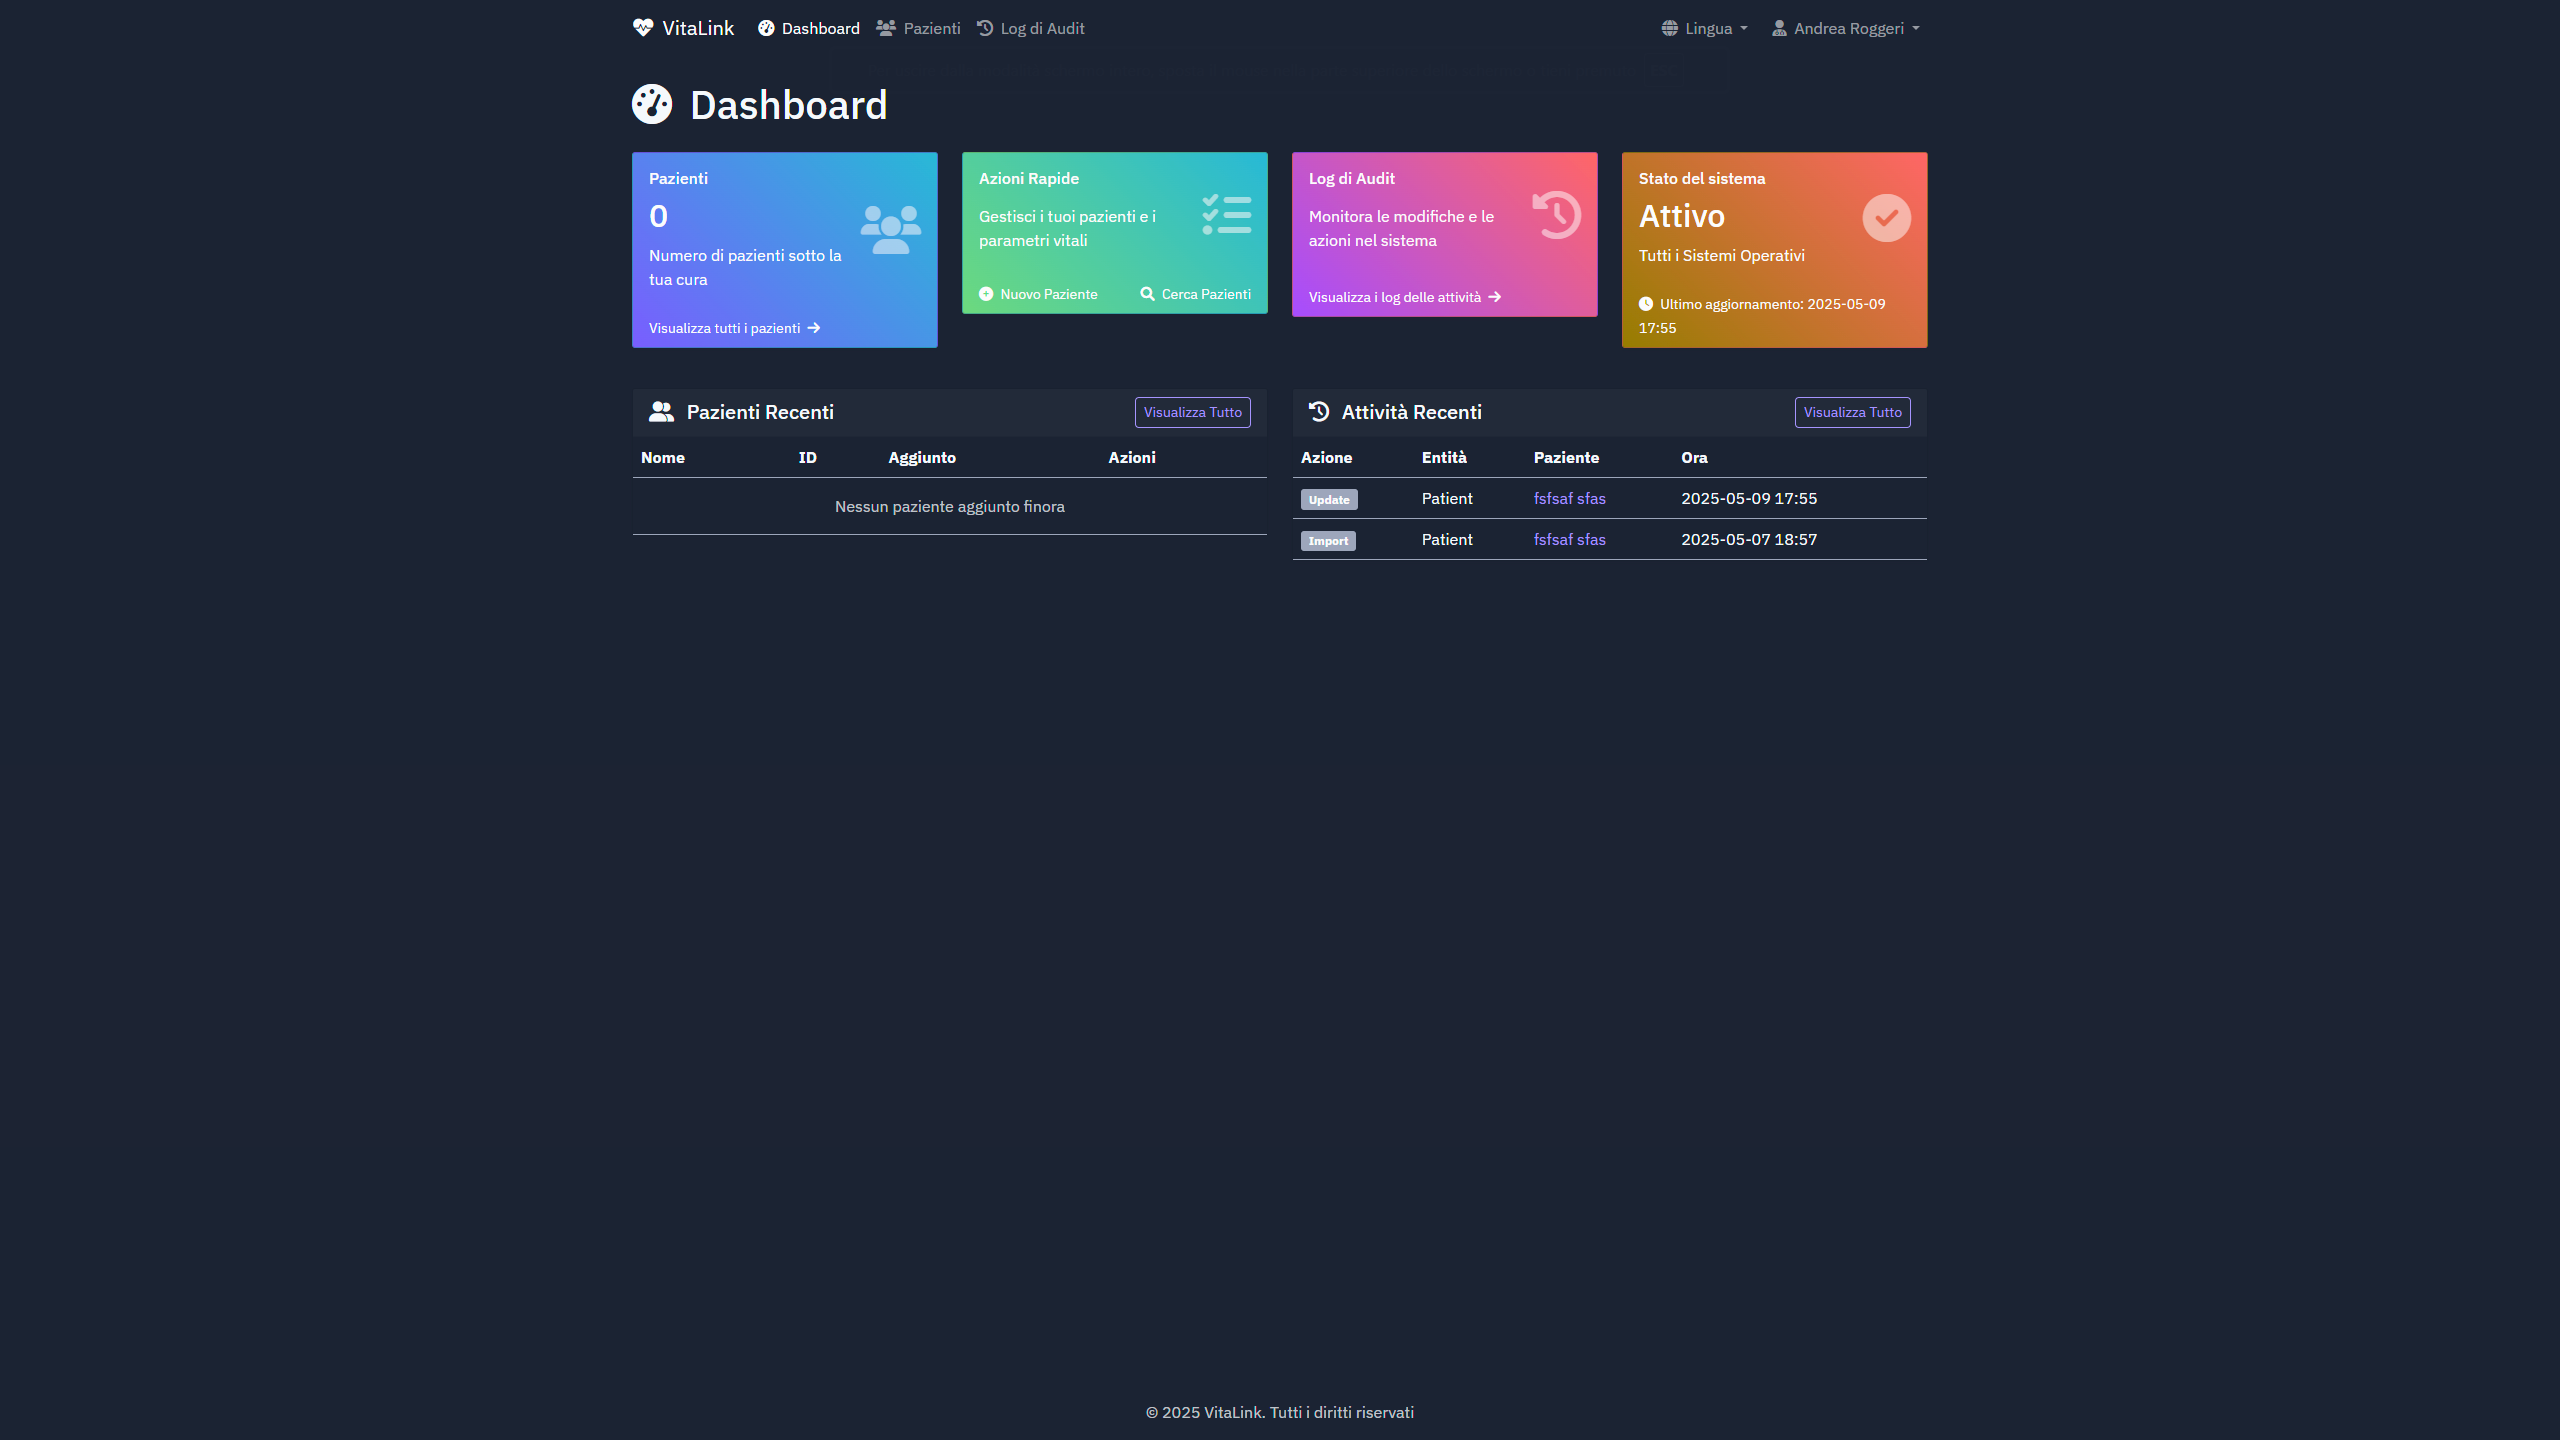
\includegraphics[width=0.85\textwidth]{images/screen/dash.png}
    \caption{Dashboard principale: pagina iniziale che mostra una panoramica dei pazienti e delle attività recenti}
    \label{fig:dashboard}
\end{figure}

\begin{figure}[H]
    \centering
    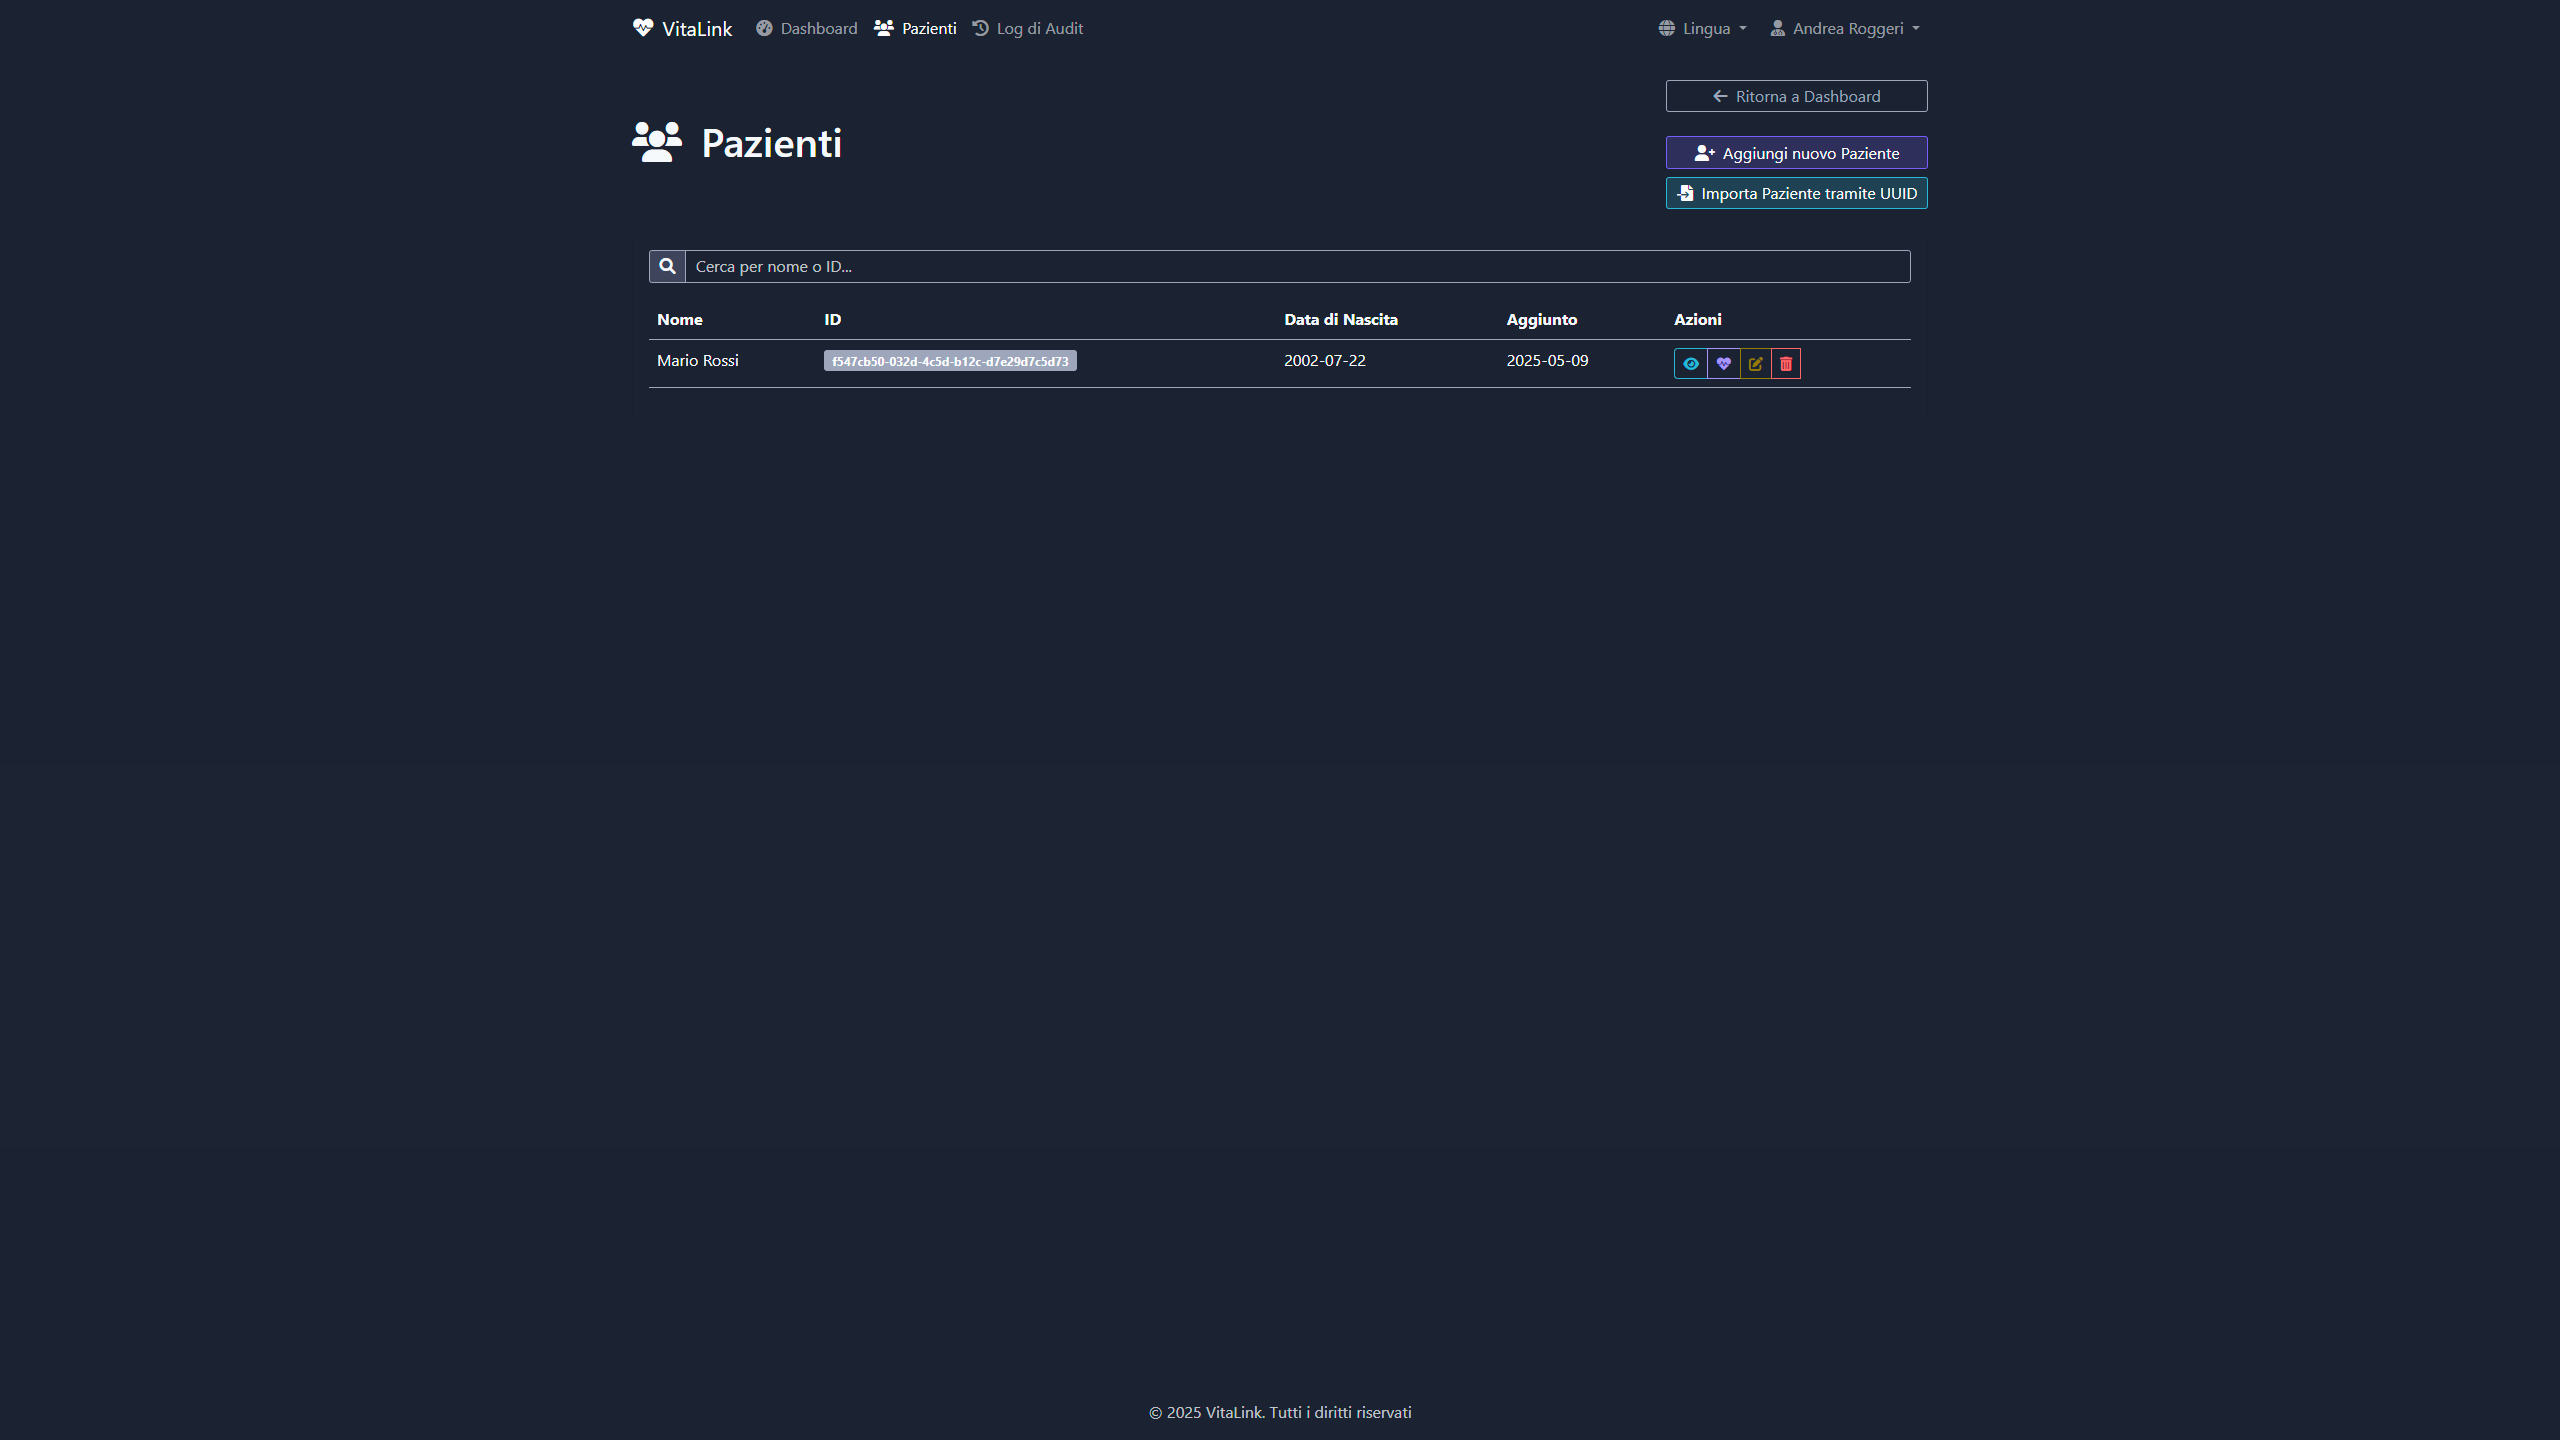
\includegraphics[width=0.85\textwidth]{images/screen/list.png}
    \caption{Lista dei pazienti: interfaccia per la visualizzazione e la gestione di tutti i pazienti seguiti dal medico}
    \label{fig:patient-list}
\end{figure}

\begin{figure}[H]
    \centering
    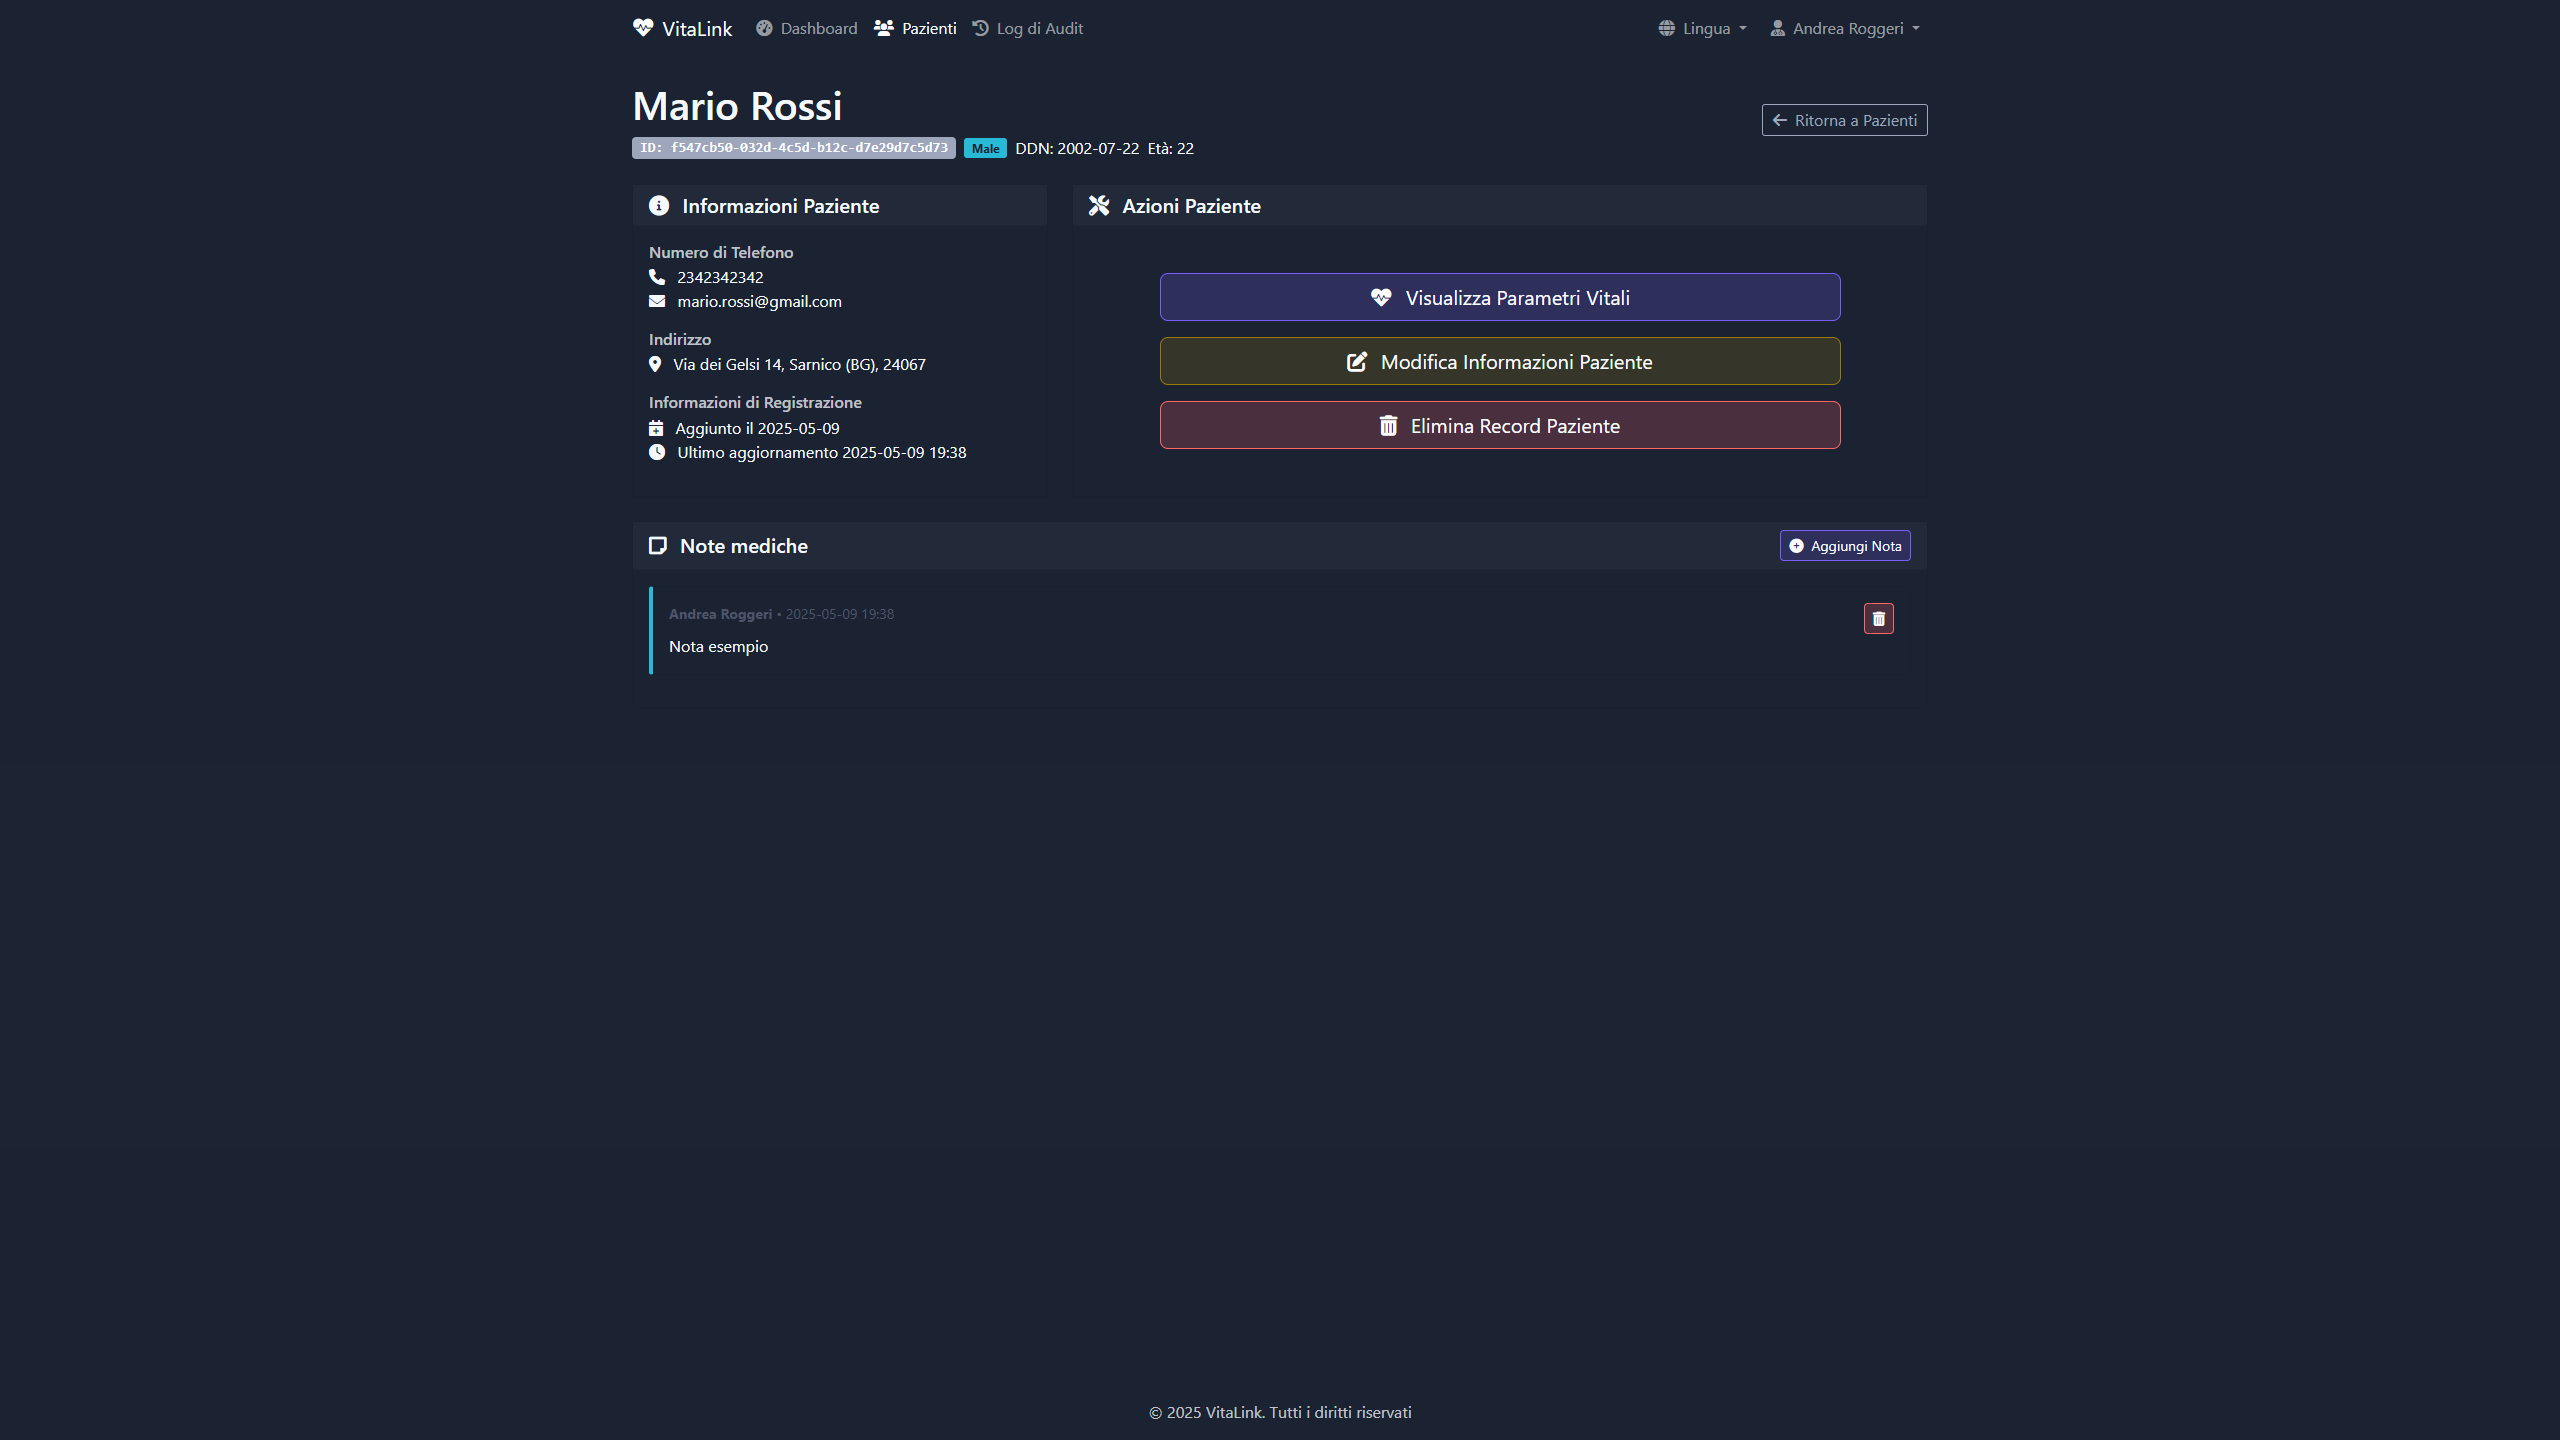
\includegraphics[width=0.85\textwidth]{images/screen/details.png}
  \caption{Dettaglio paziente: schermata con le informazioni dettagliate e le note mediche relative ad un paziente specifico}
    \label{fig:patient-details}
\end{figure}

\begin{figure}[H]
    \centering
    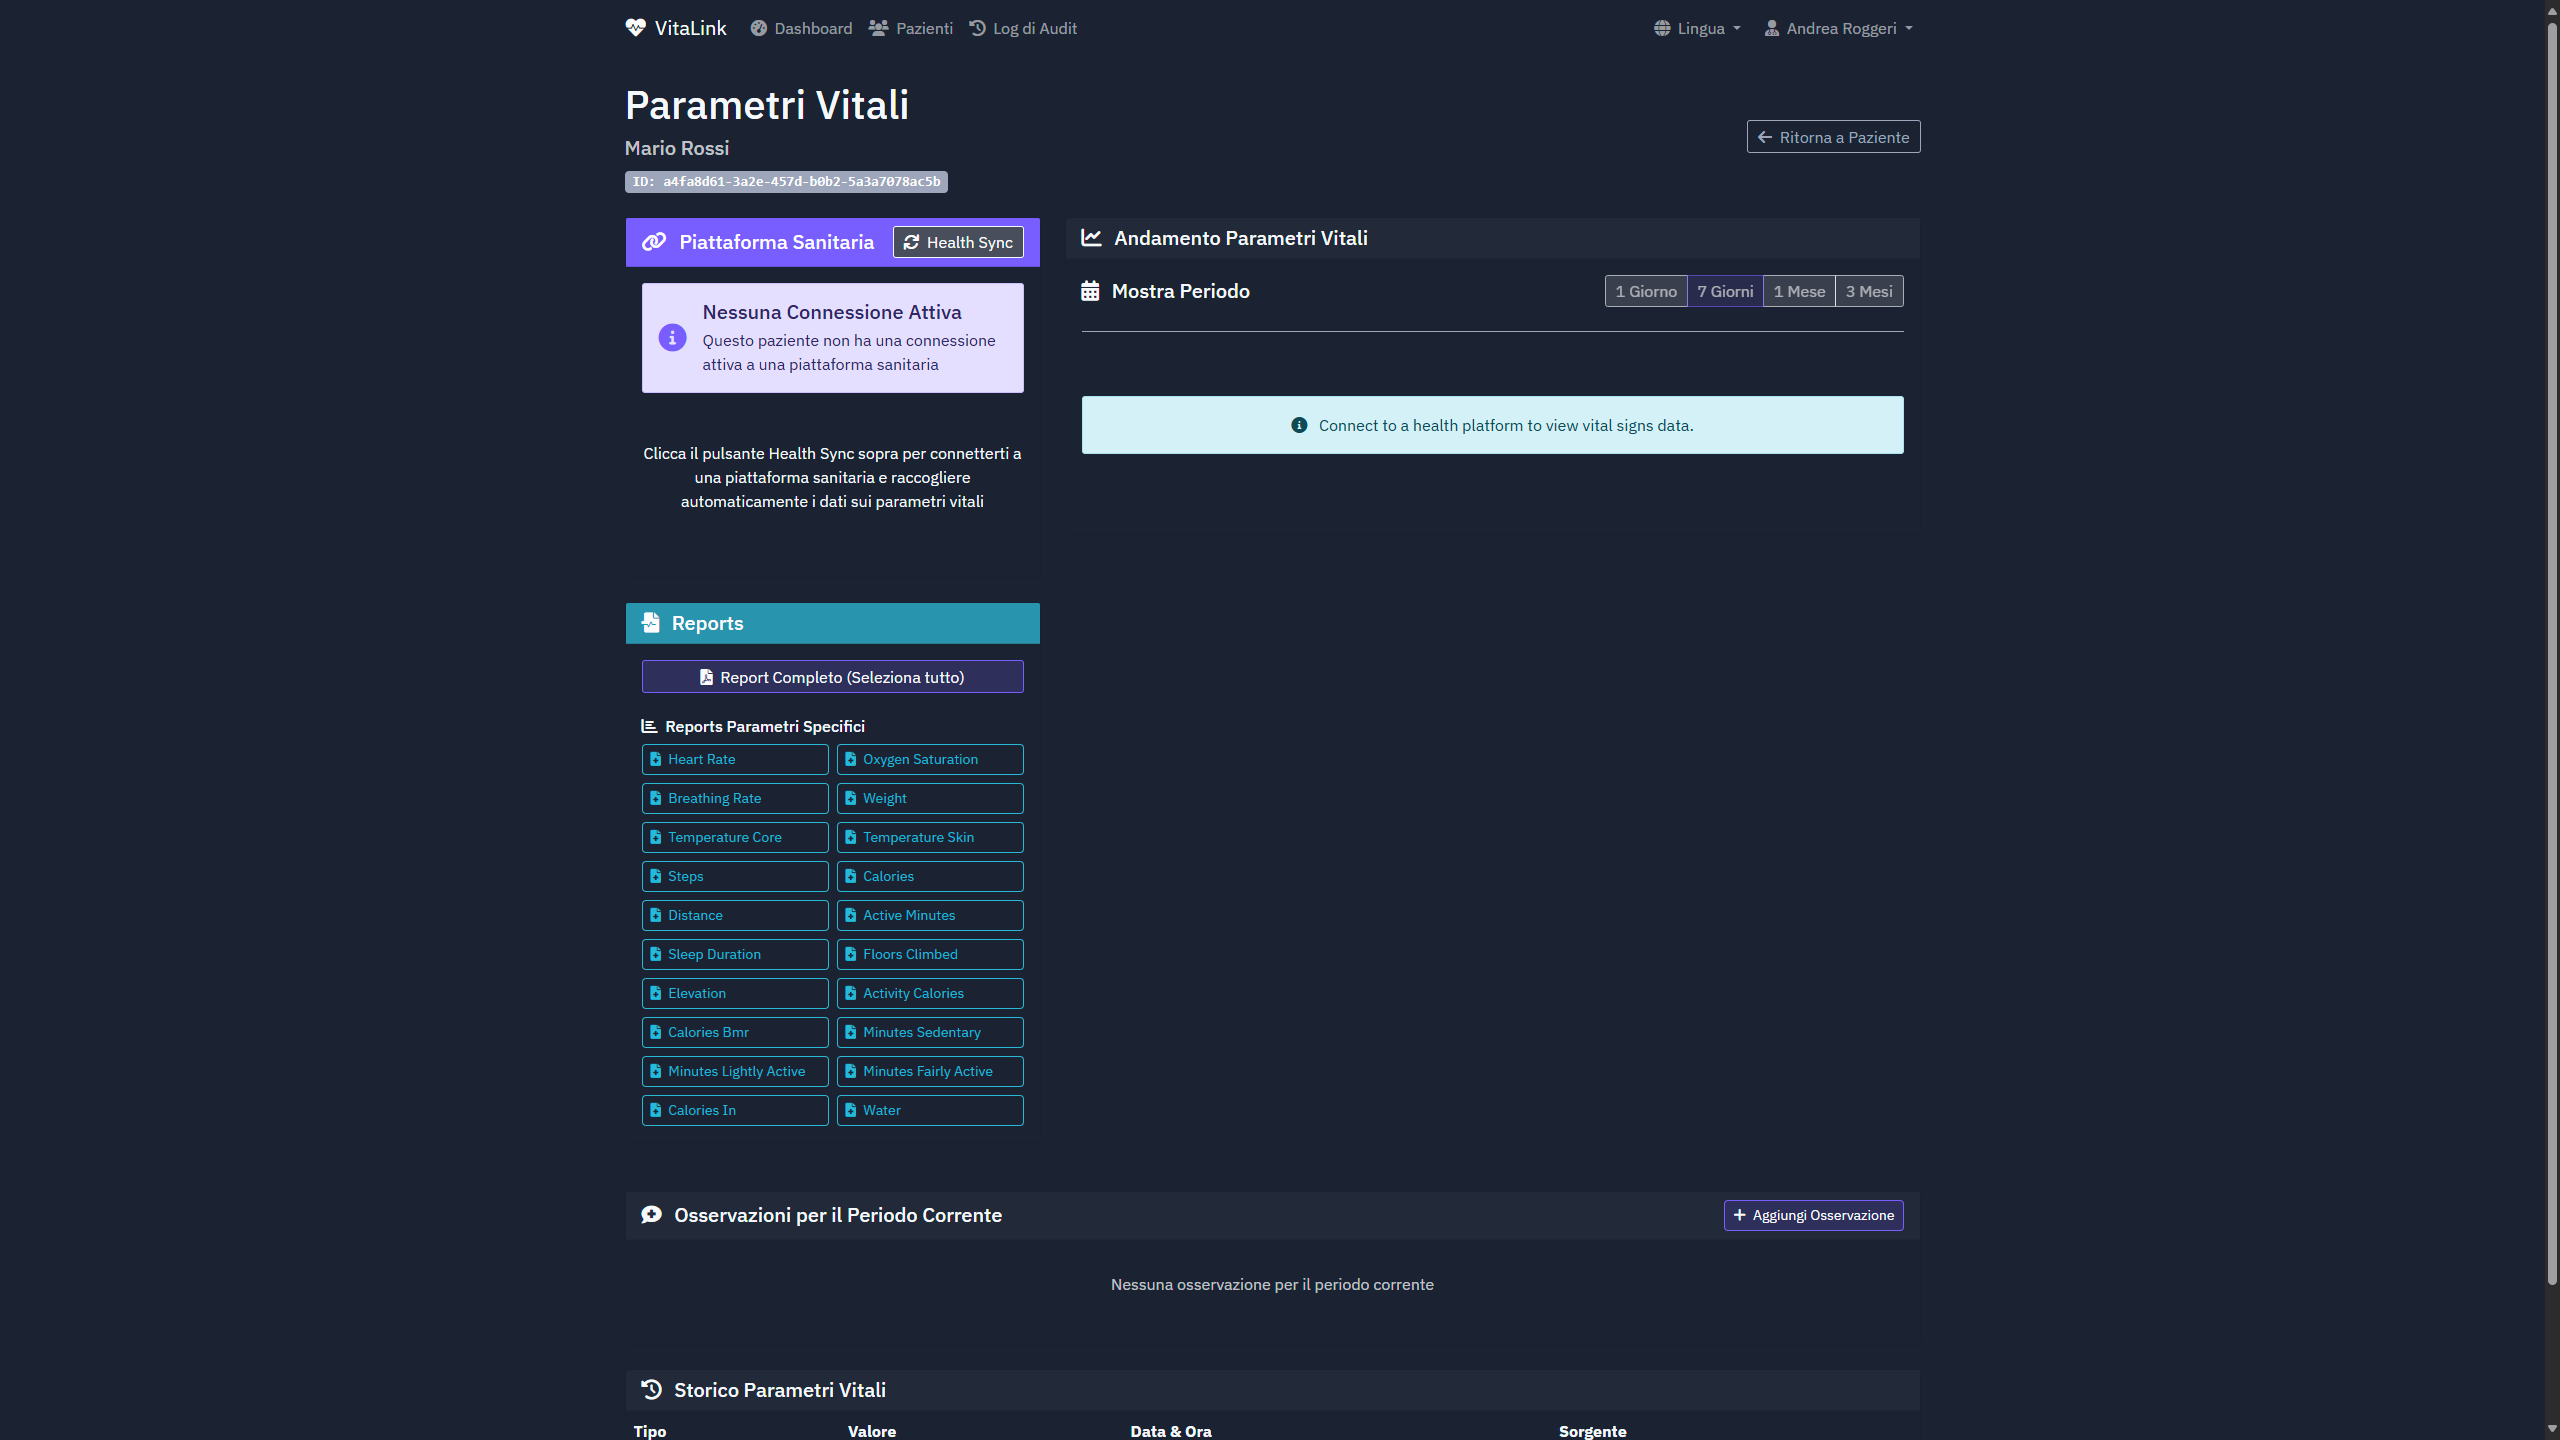
\includegraphics[width=0.85\textwidth]{images/screen/unconnected.png}
    \caption{Parametri vitali (dispositivo non connesso): stato iniziale della pagina dei parametri vitali quando nessun dispositivo è collegato}
    \label{fig:unconnected}
\end{figure}

\begin{figure}[H]
    \centering
    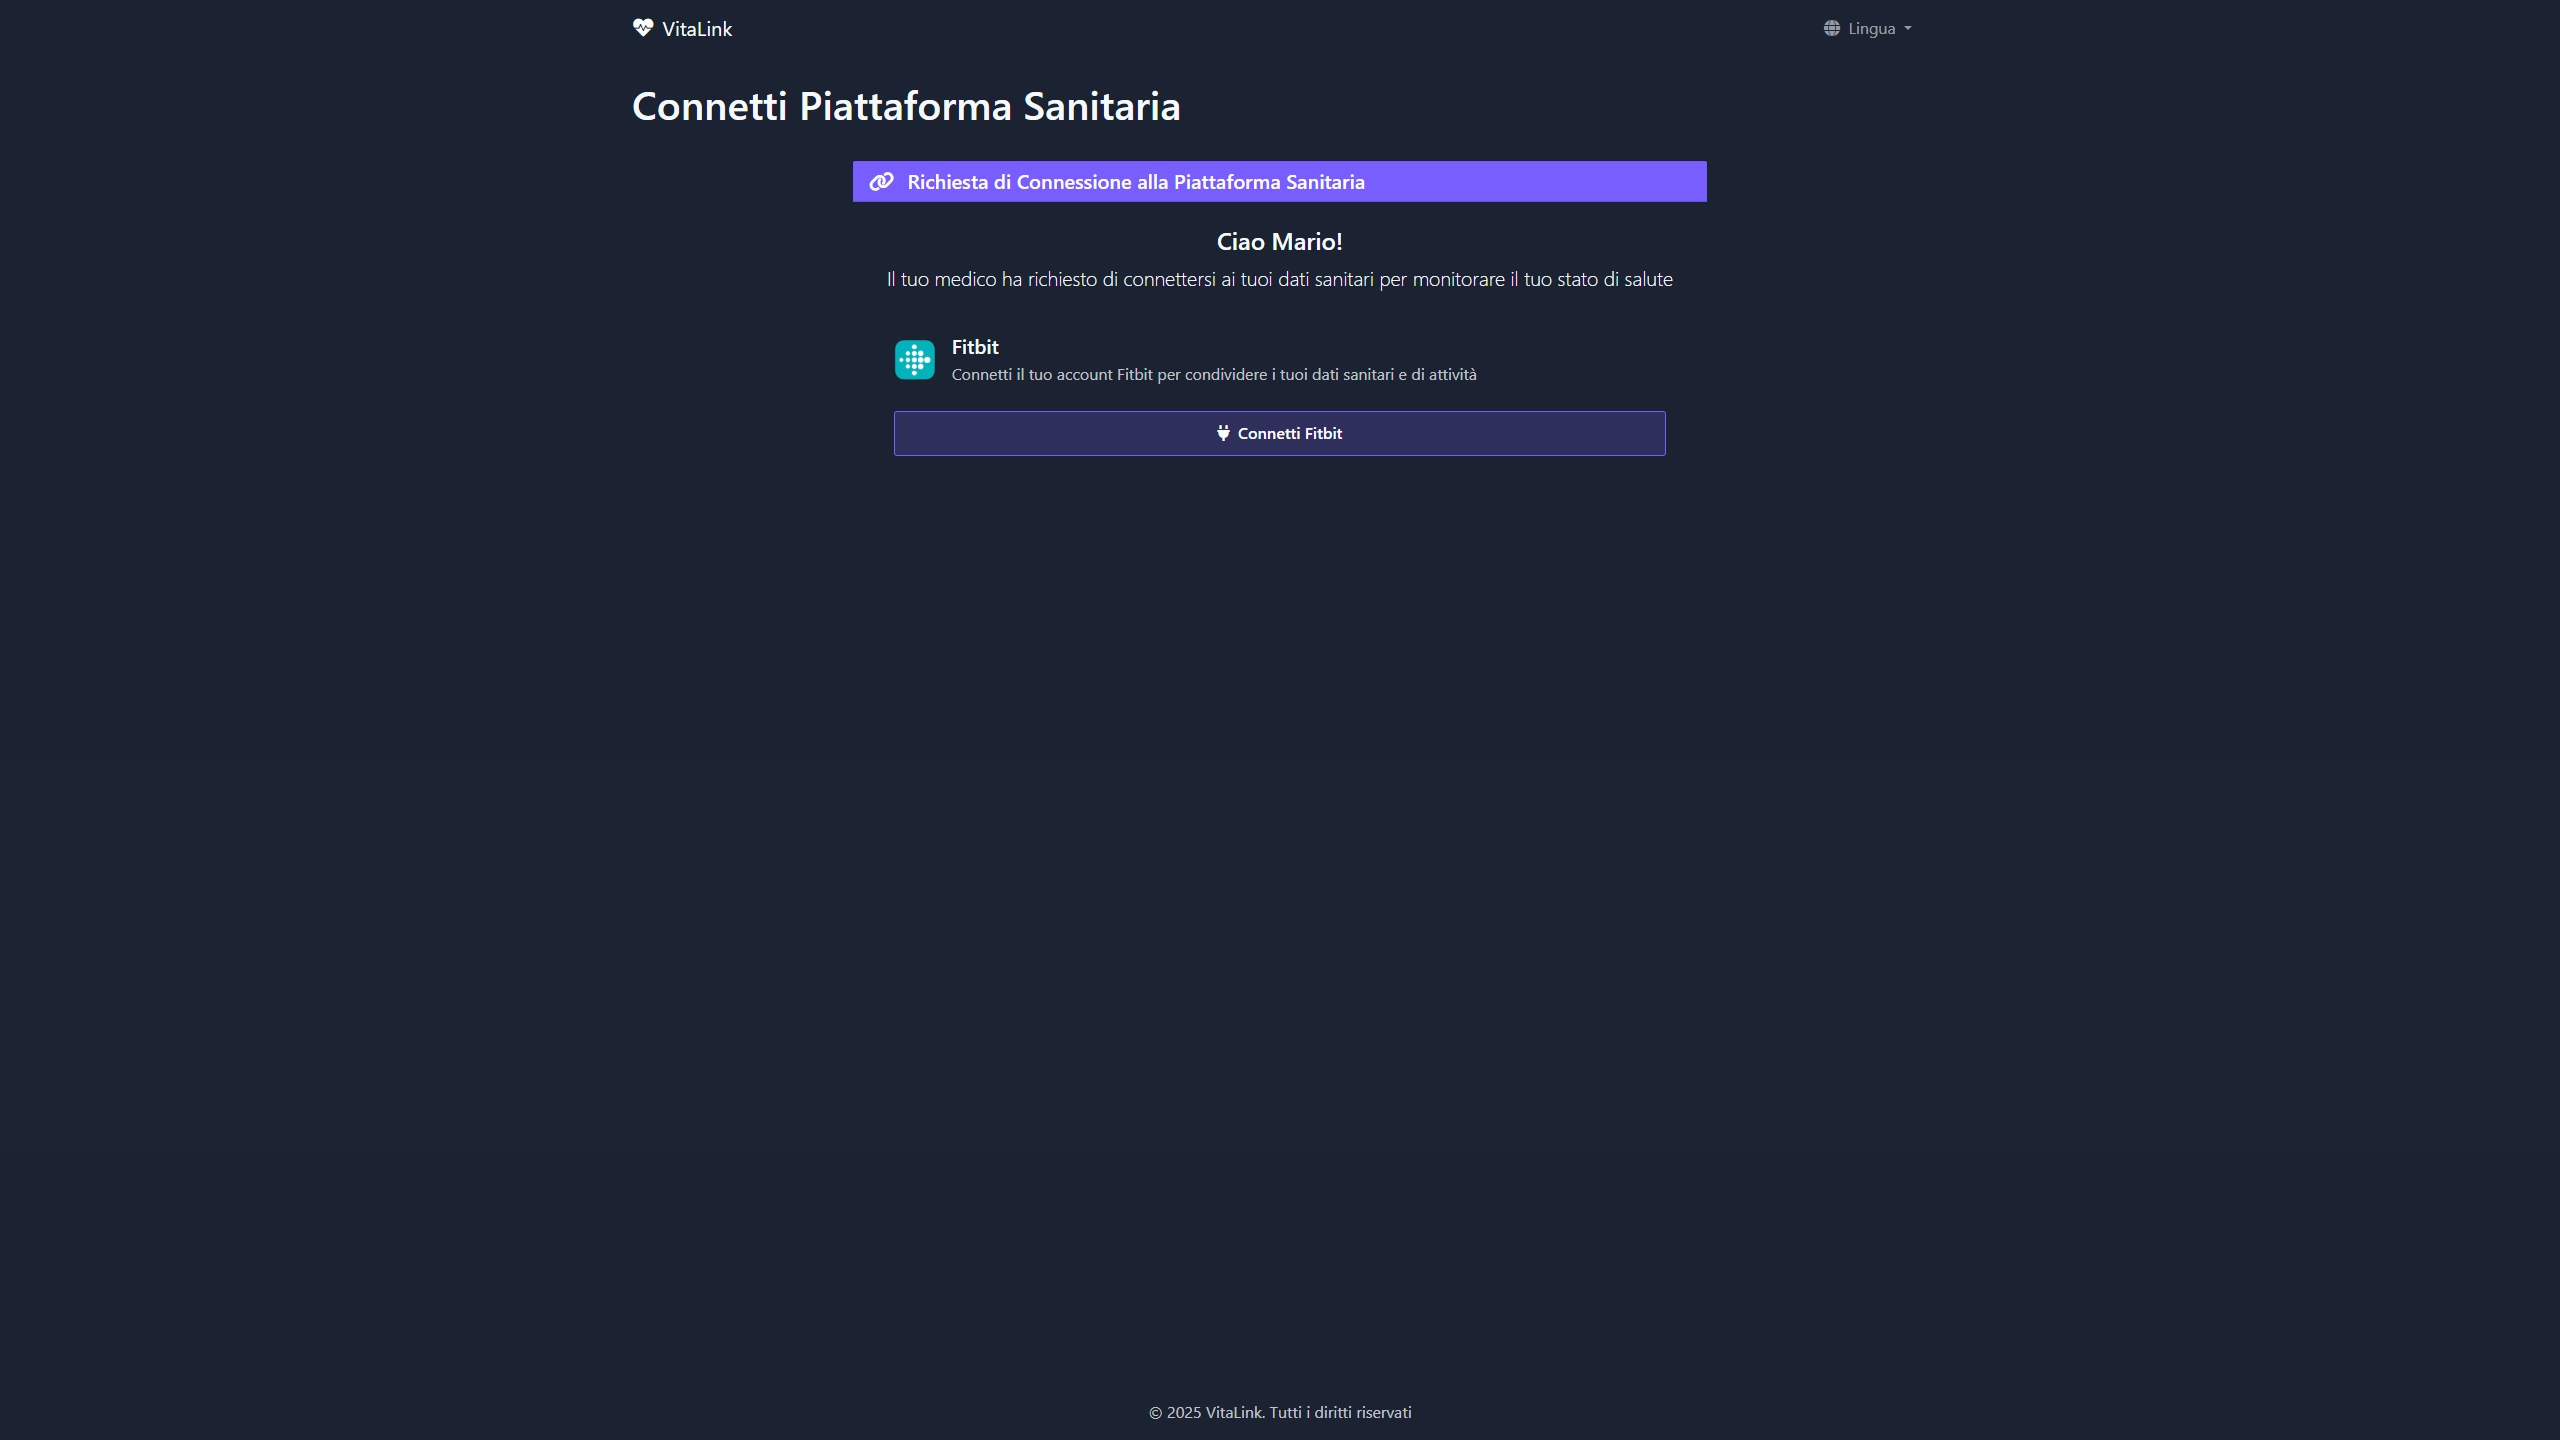
\includegraphics[width=0.85\textwidth]{images/screen/connection.png}
    \caption{Connessione dispositivo: interfaccia per l'autorizzazione e il collegamento di dispositivi wearable}
    \label{fig:connection}
\end{figure}

\begin{figure}[H]
    \centering
    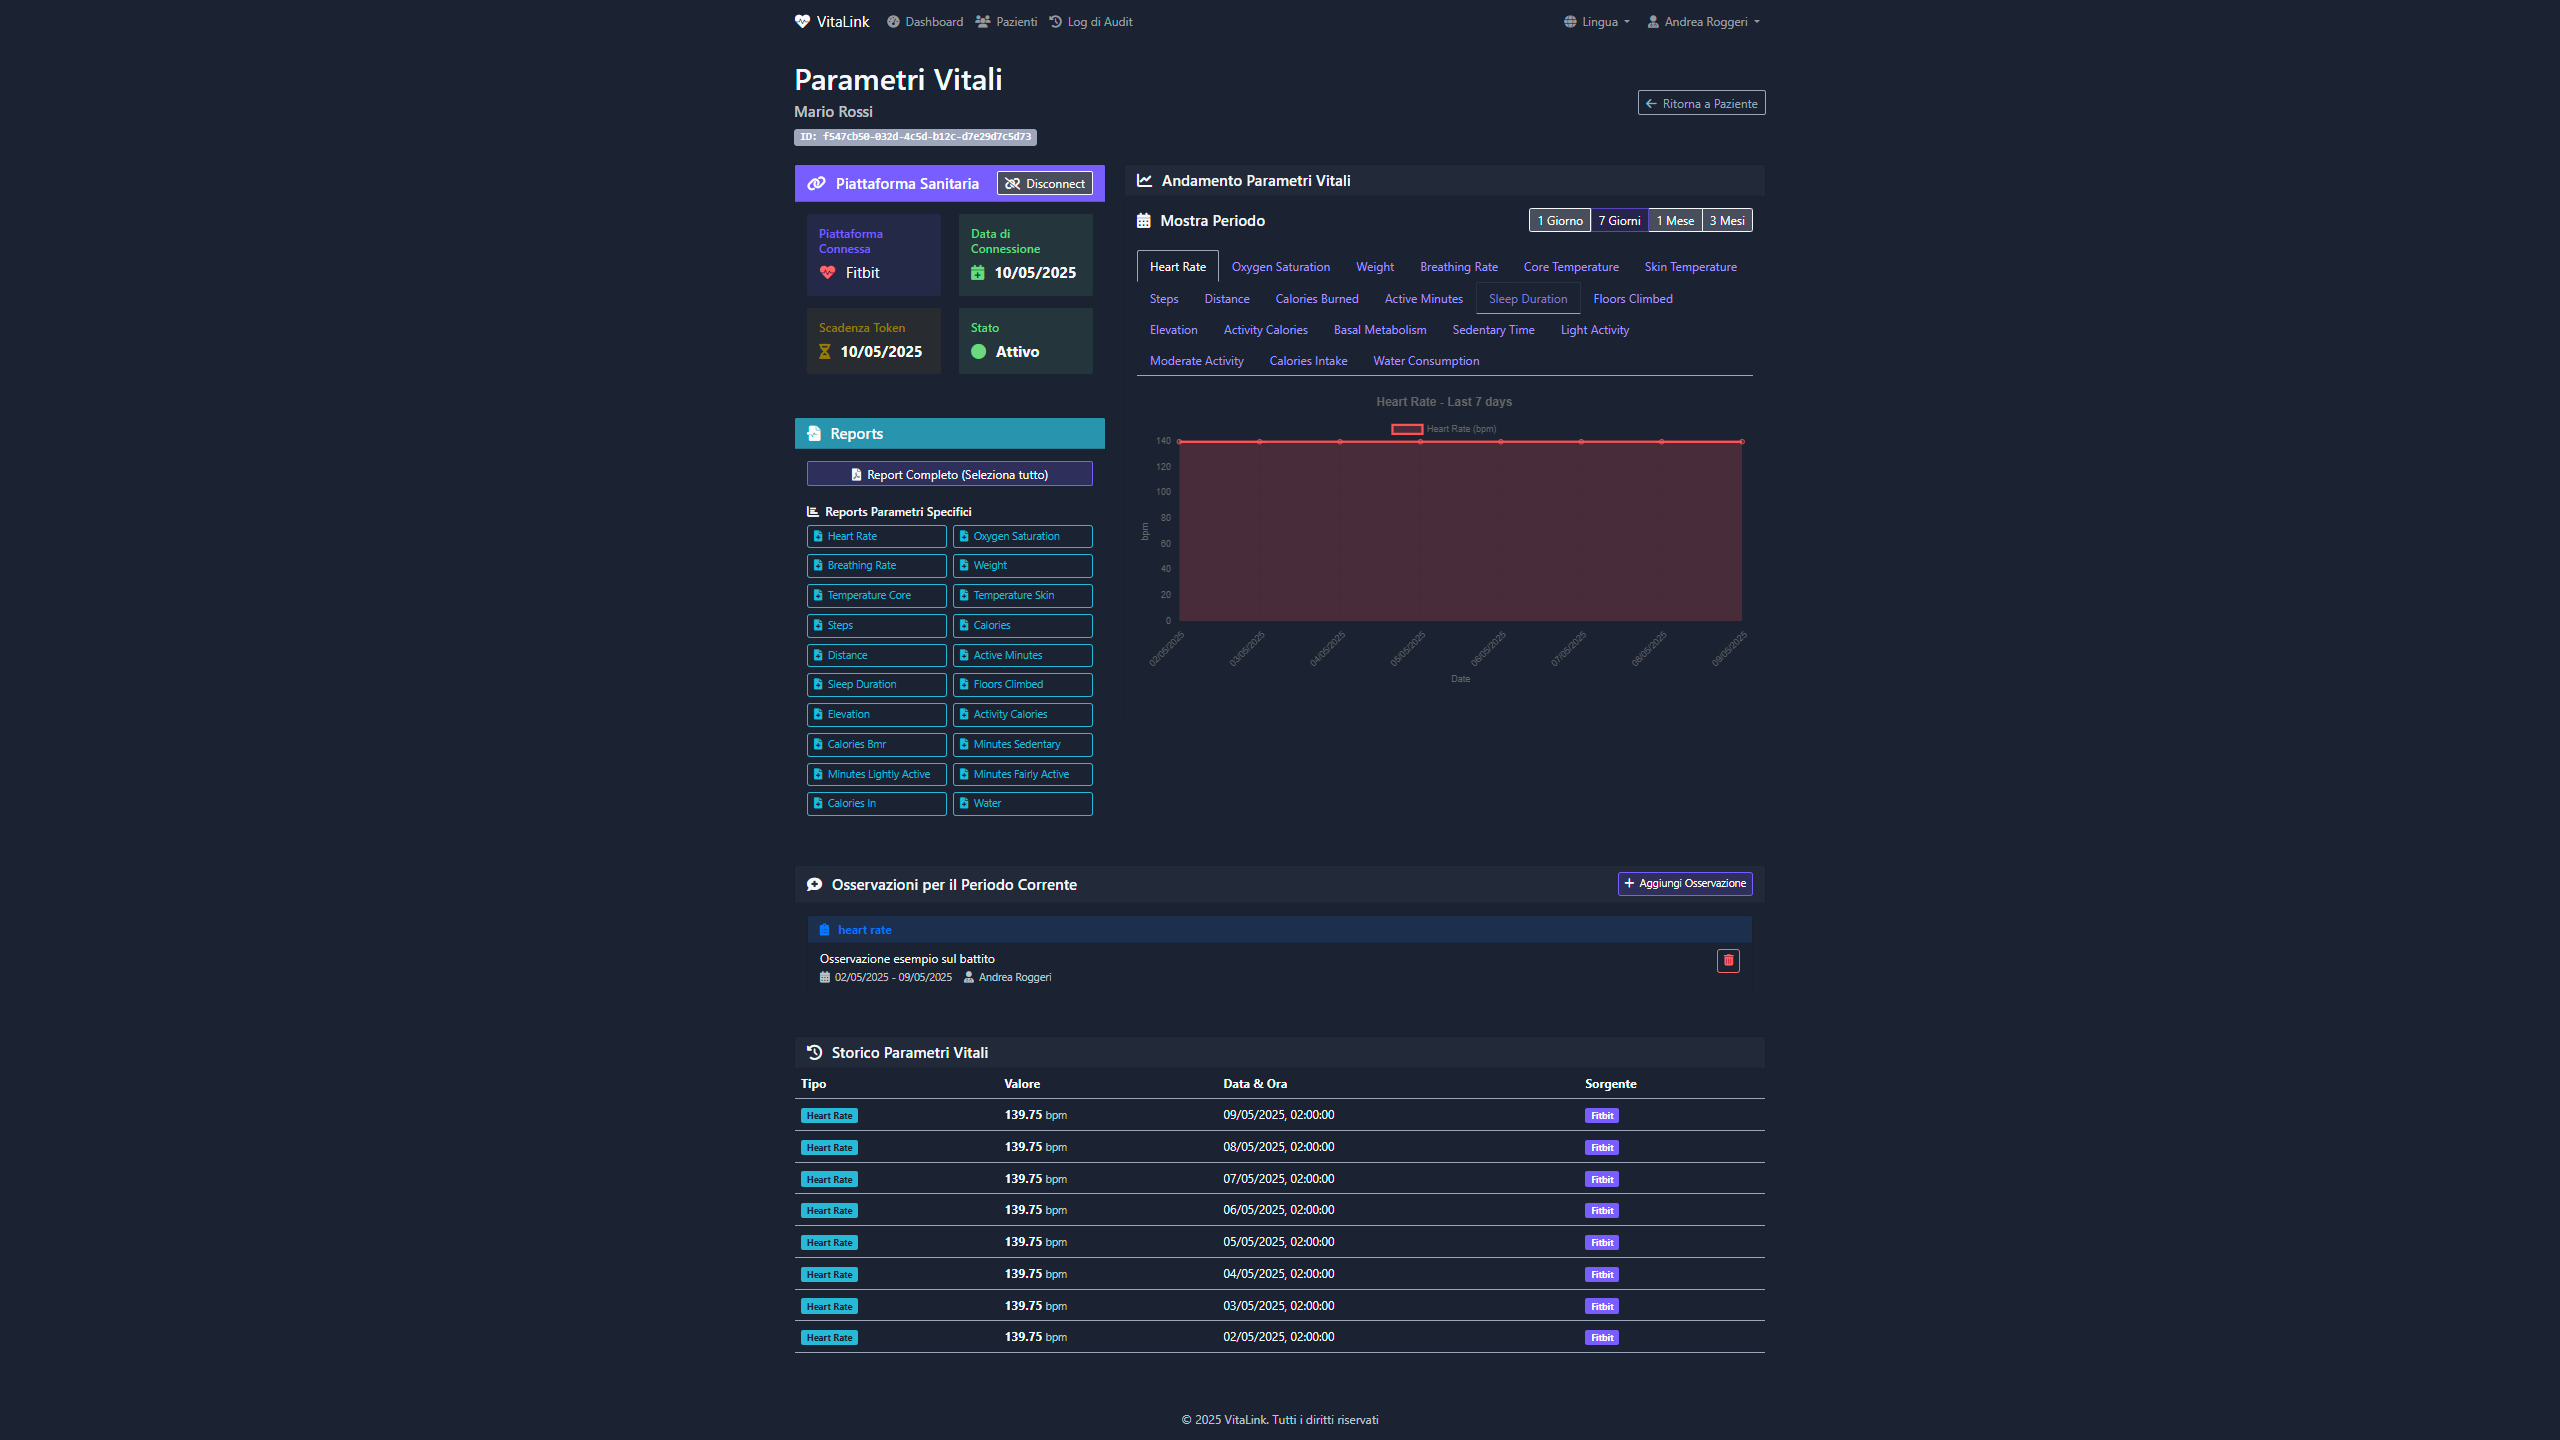
\includegraphics[width=0.85\textwidth]{images/screen/vitals.png}
    \caption{Visualizzazione parametri vitali: grafici e dati dei parametri vitali monitorati dal dispositivo collegato}
    \label{fig:vitals}
\end{figure}

\begin{figure}[H]
    \centering
    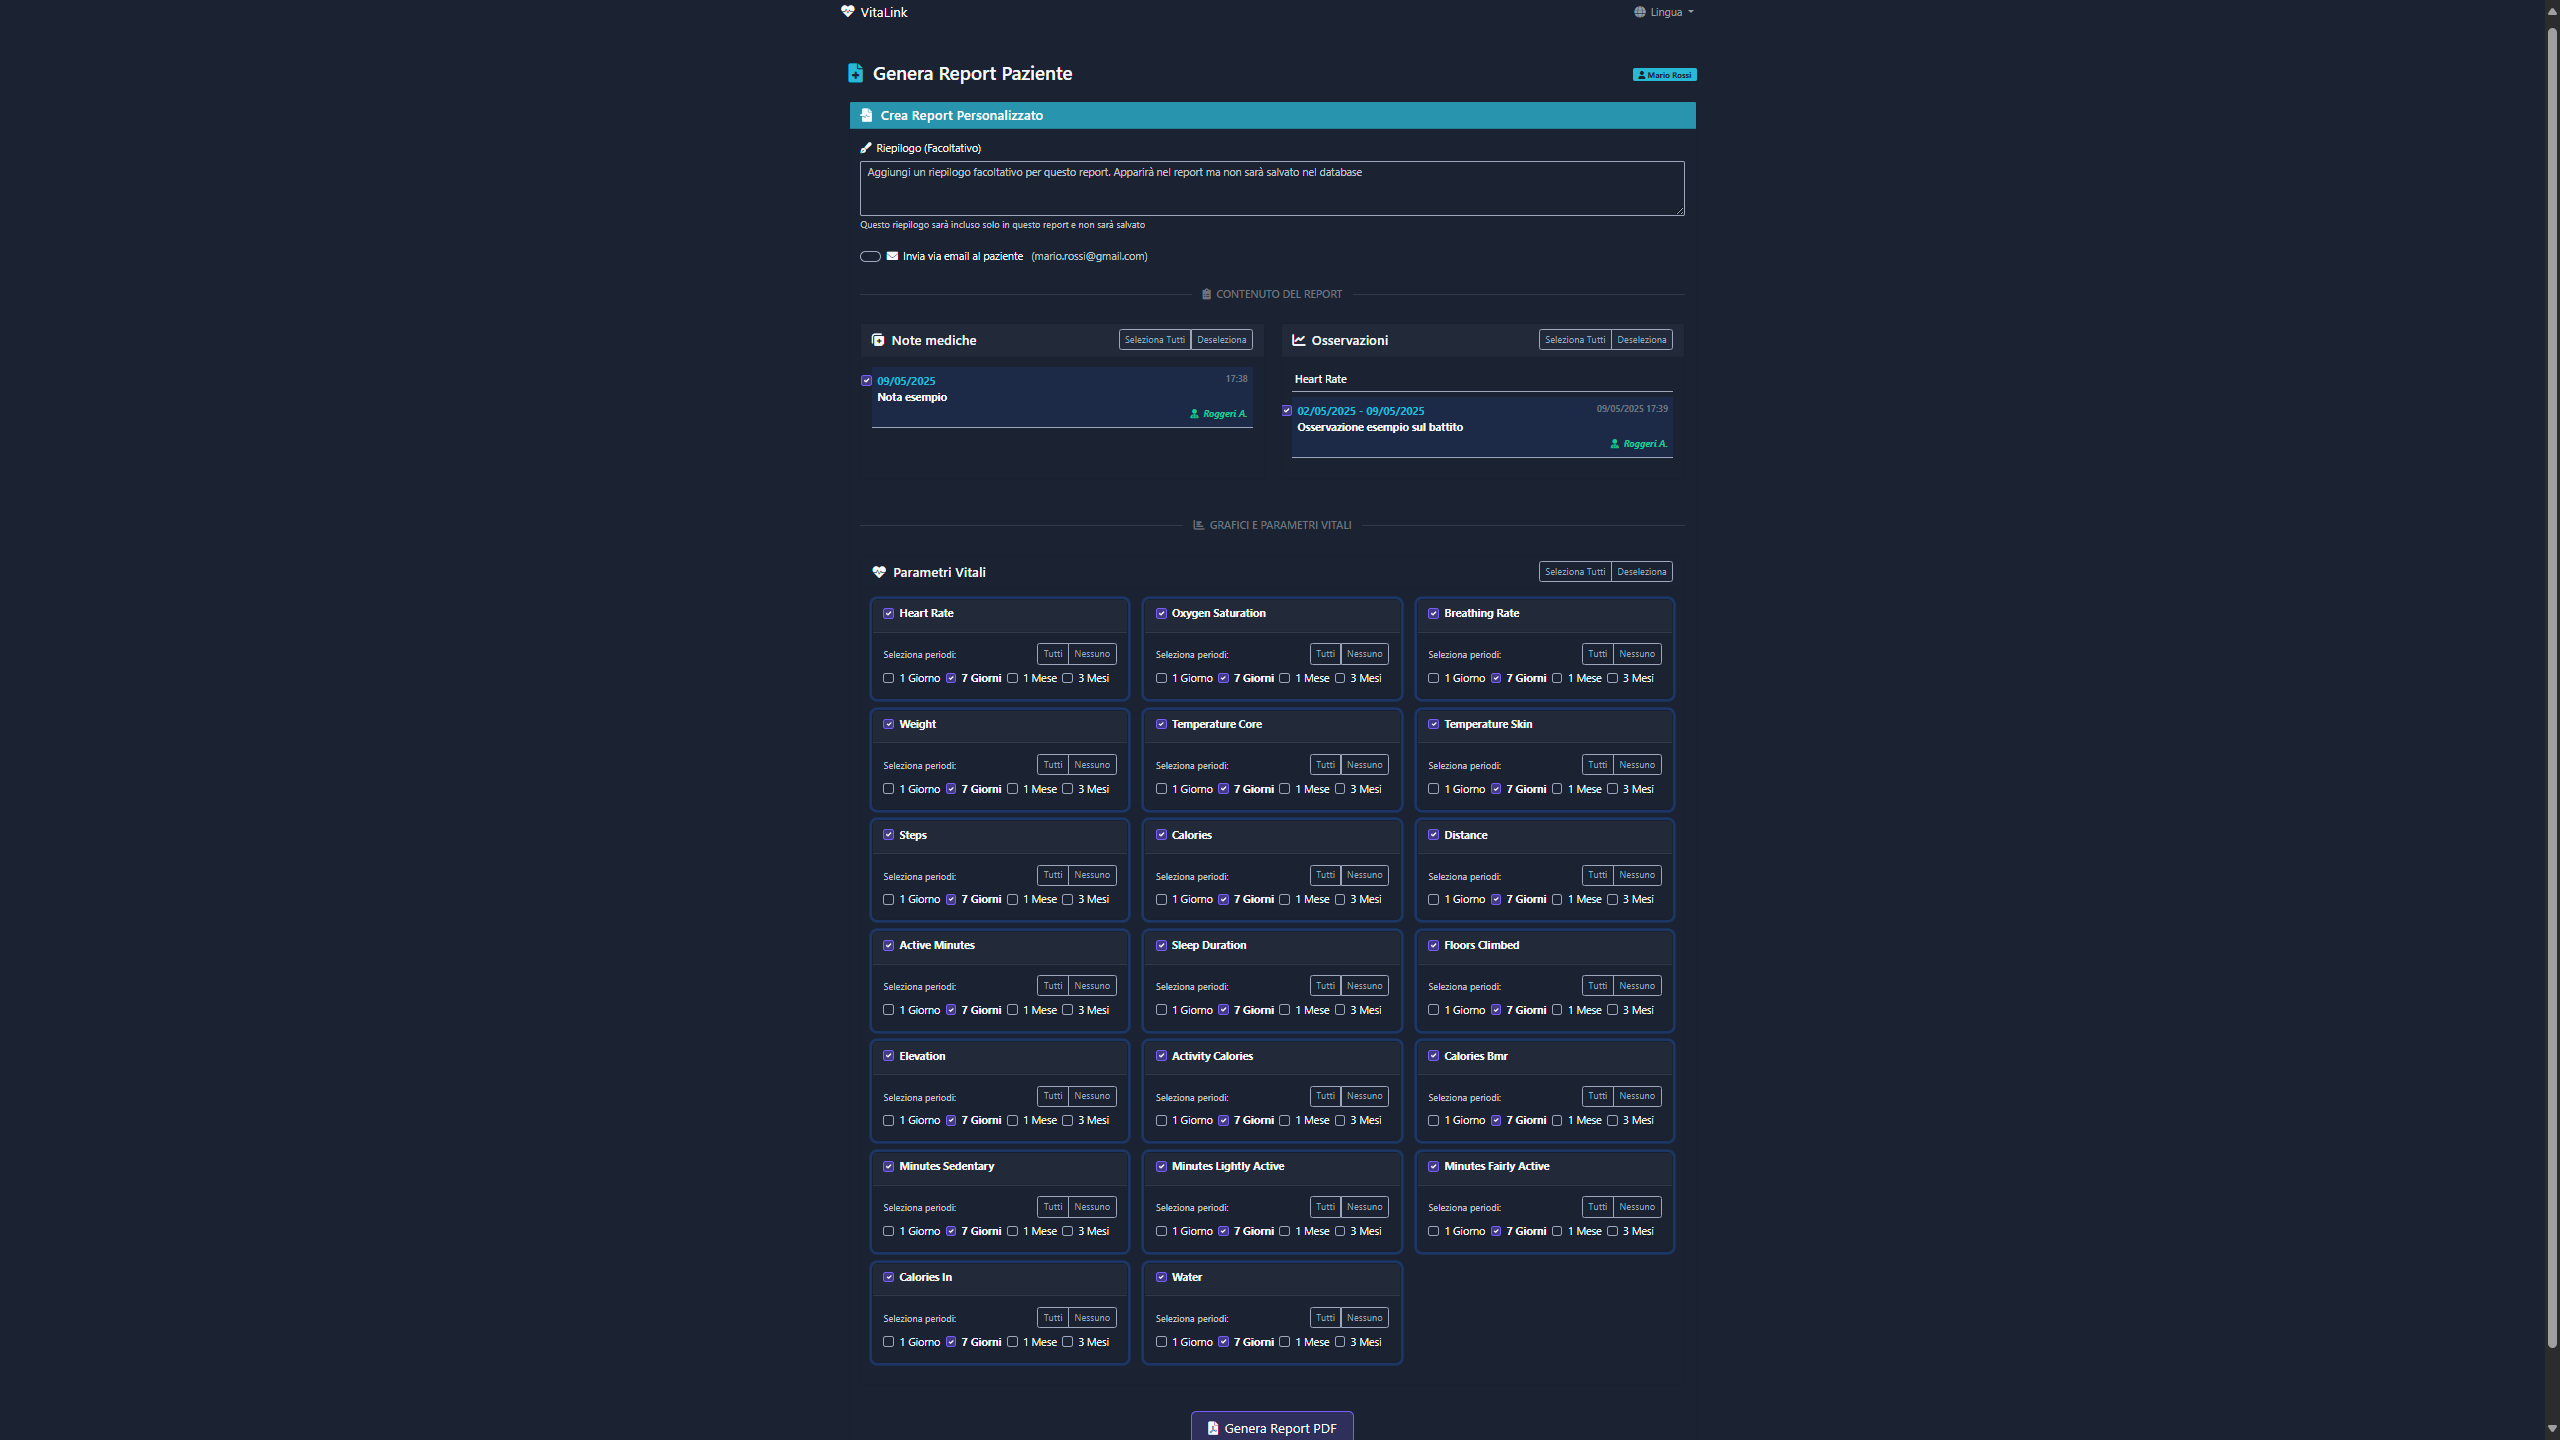
\includegraphics[width=0.85\textwidth]{images/screen/report.png}
    \caption{Generazione report: interfaccia per la creazione di report personalizzati sui parametri vitali del paziente}
    \label{fig:report}
\end{figure}

\begin{figure}[H]
    \centering
    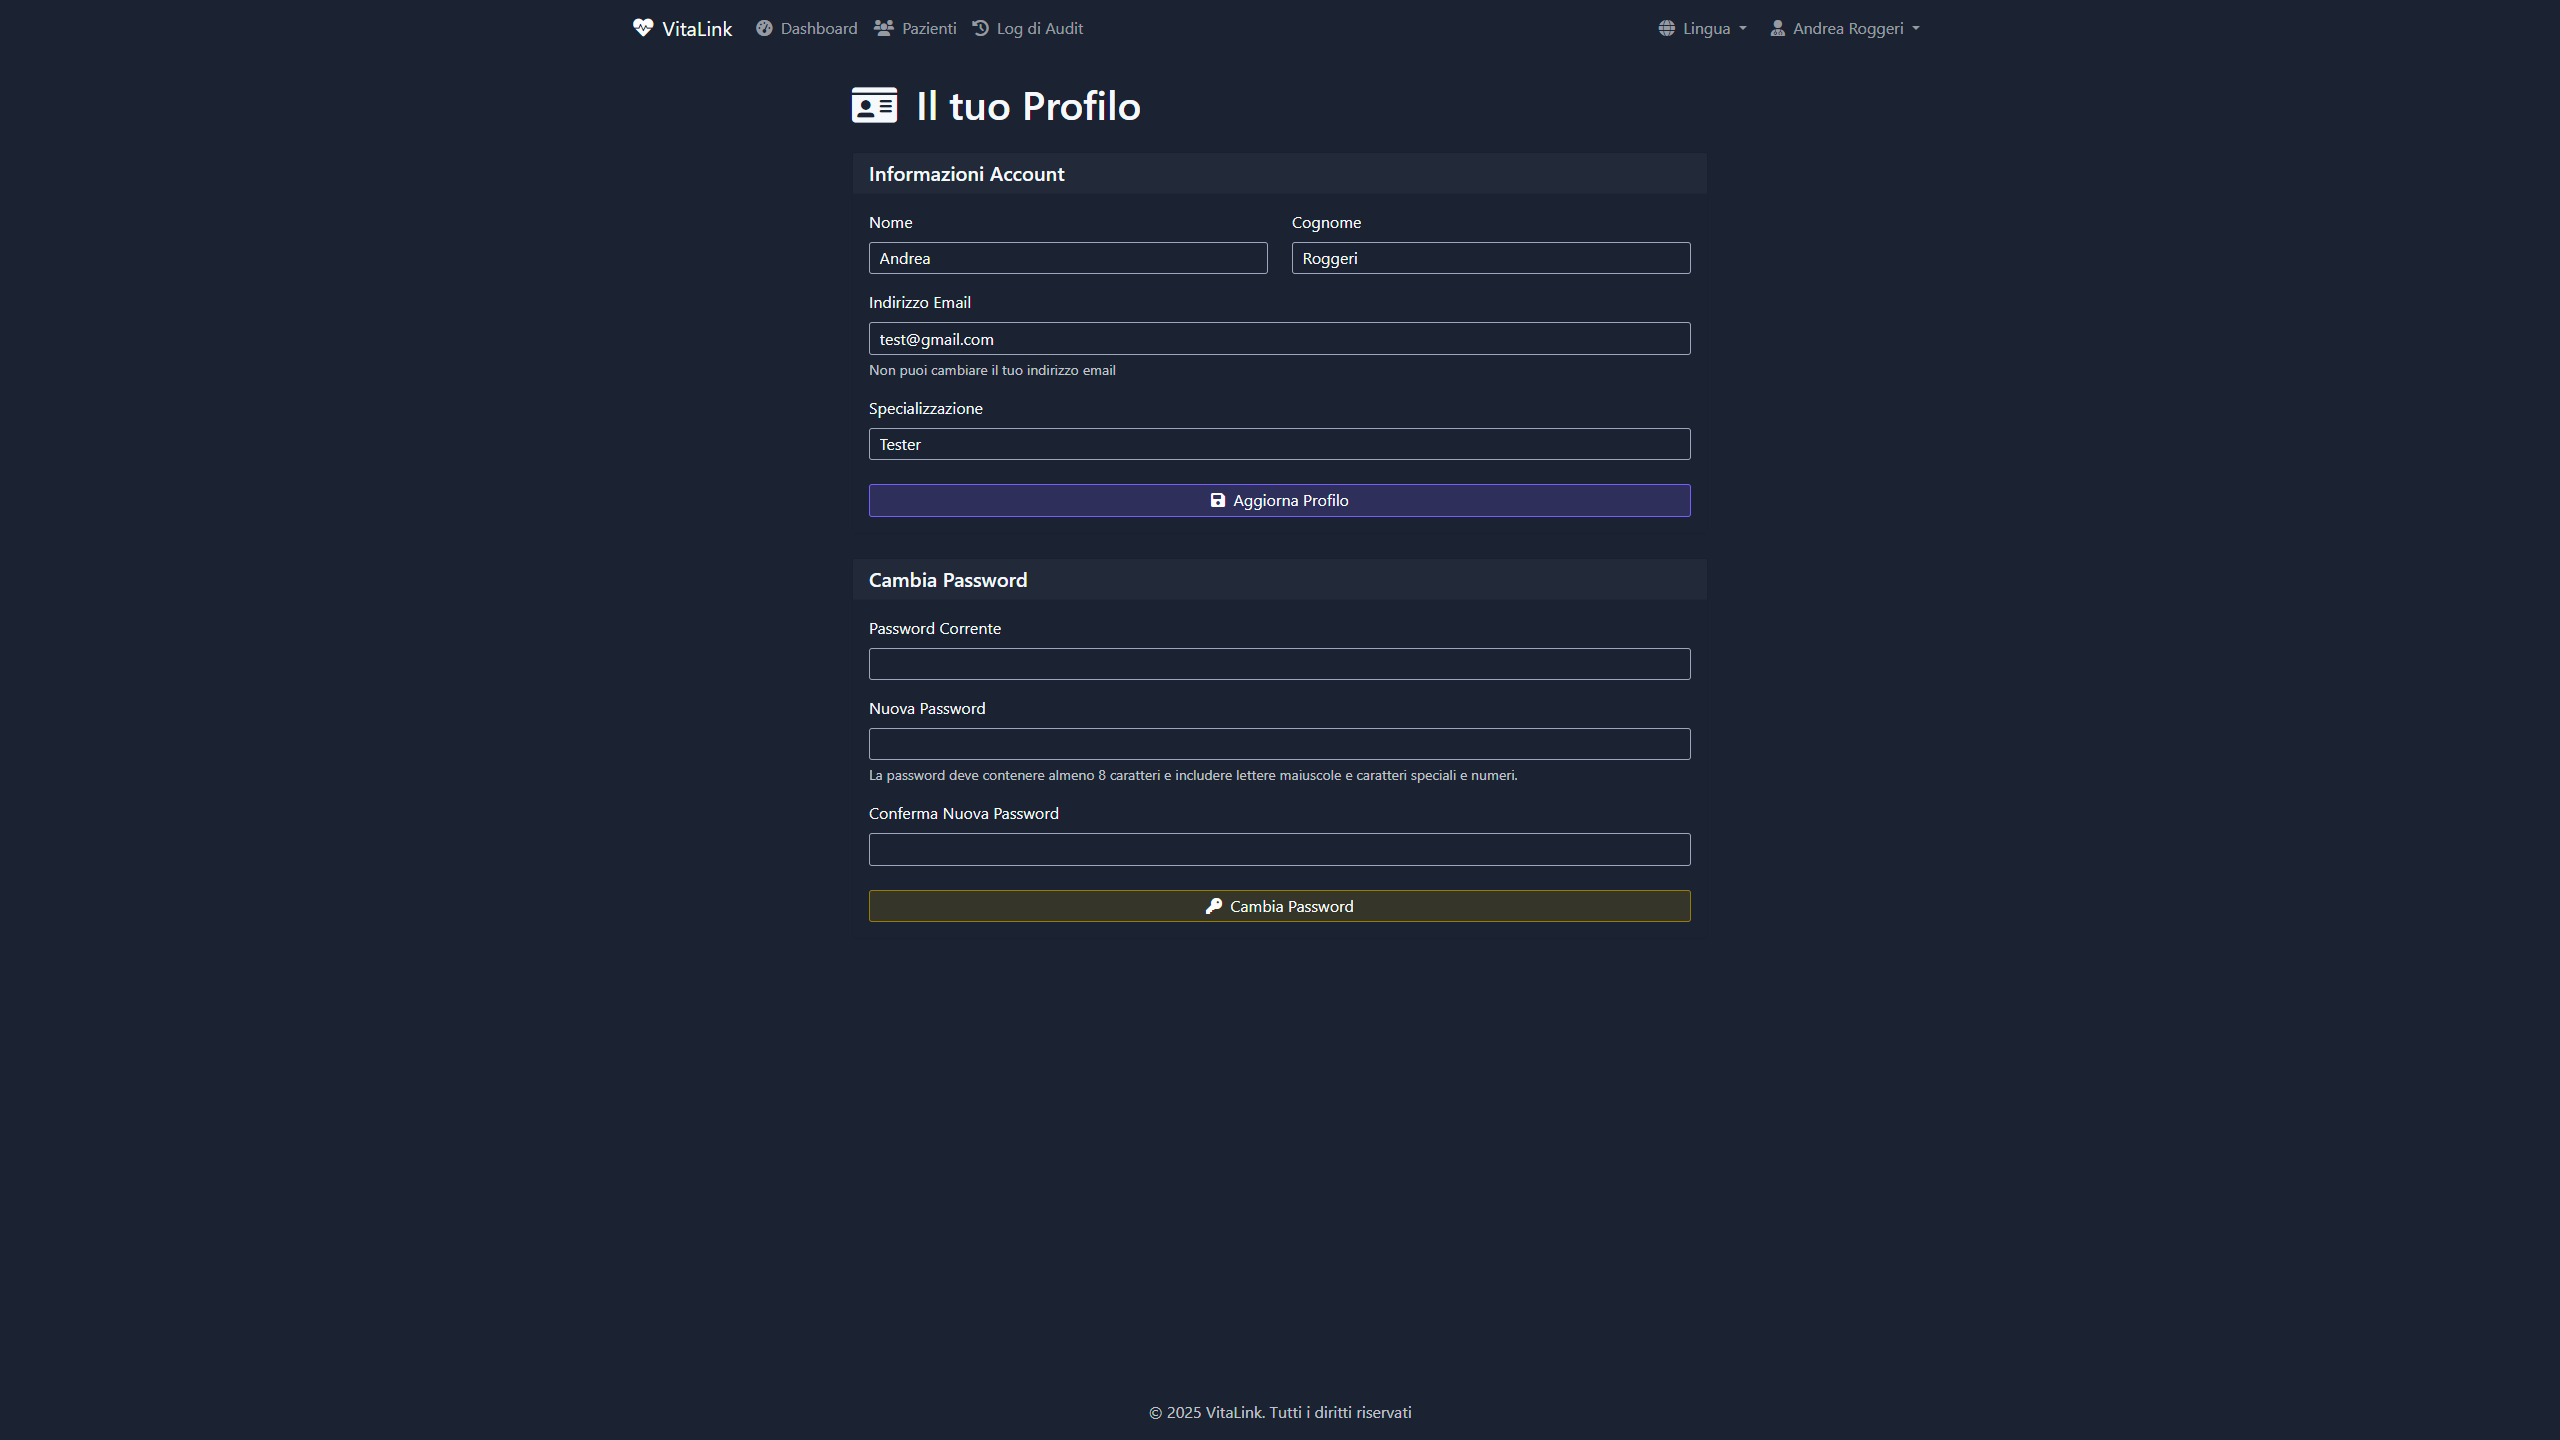
\includegraphics[width=0.85\textwidth]{images/screen/profile.png}
    \caption{Profilo utente: schermata per la gestione del profilo del medico e delle impostazioni personali}
    \label{fig:profile}
\end{figure}

\begin{figure}[H]
    \centering
    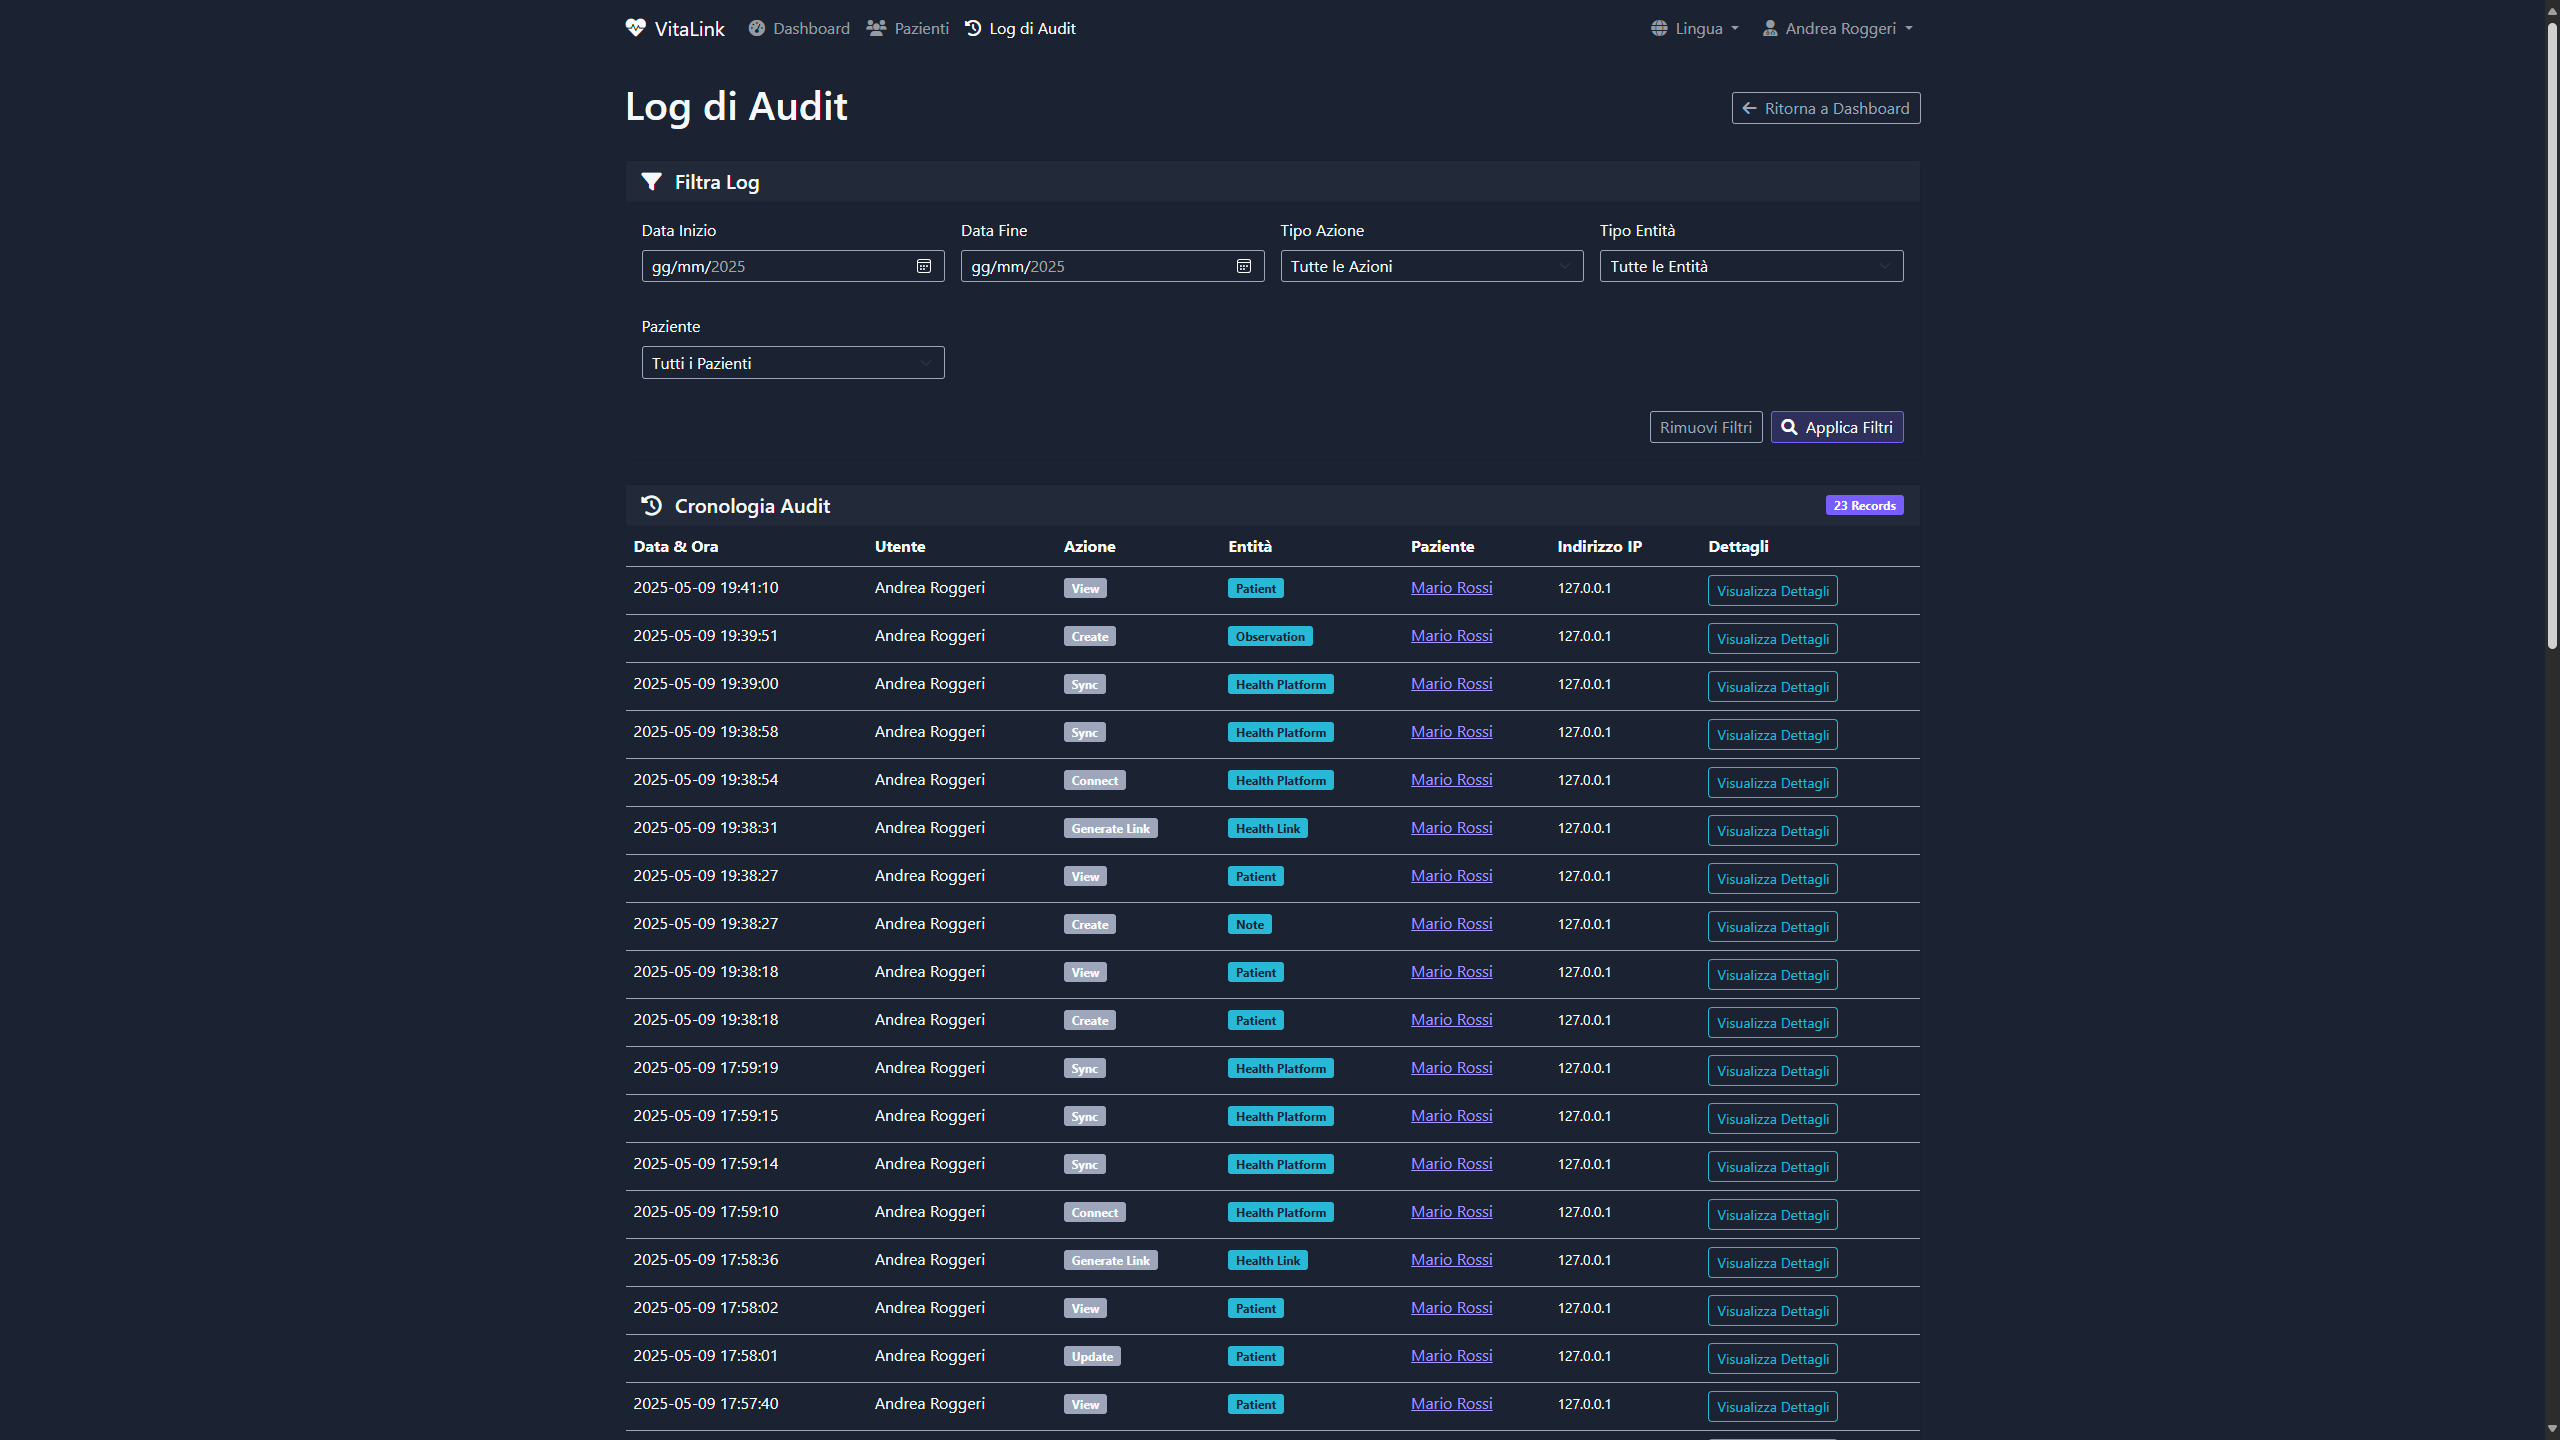
\includegraphics[width=0.85\textwidth]{images/screen/audit list.png}
    \caption{Log di audit: lista delle attività e delle modifiche effettuate sui dati dei pazienti}
    \label{fig:audit-list}
\end{figure}

\begin{figure}[H]
    \centering
    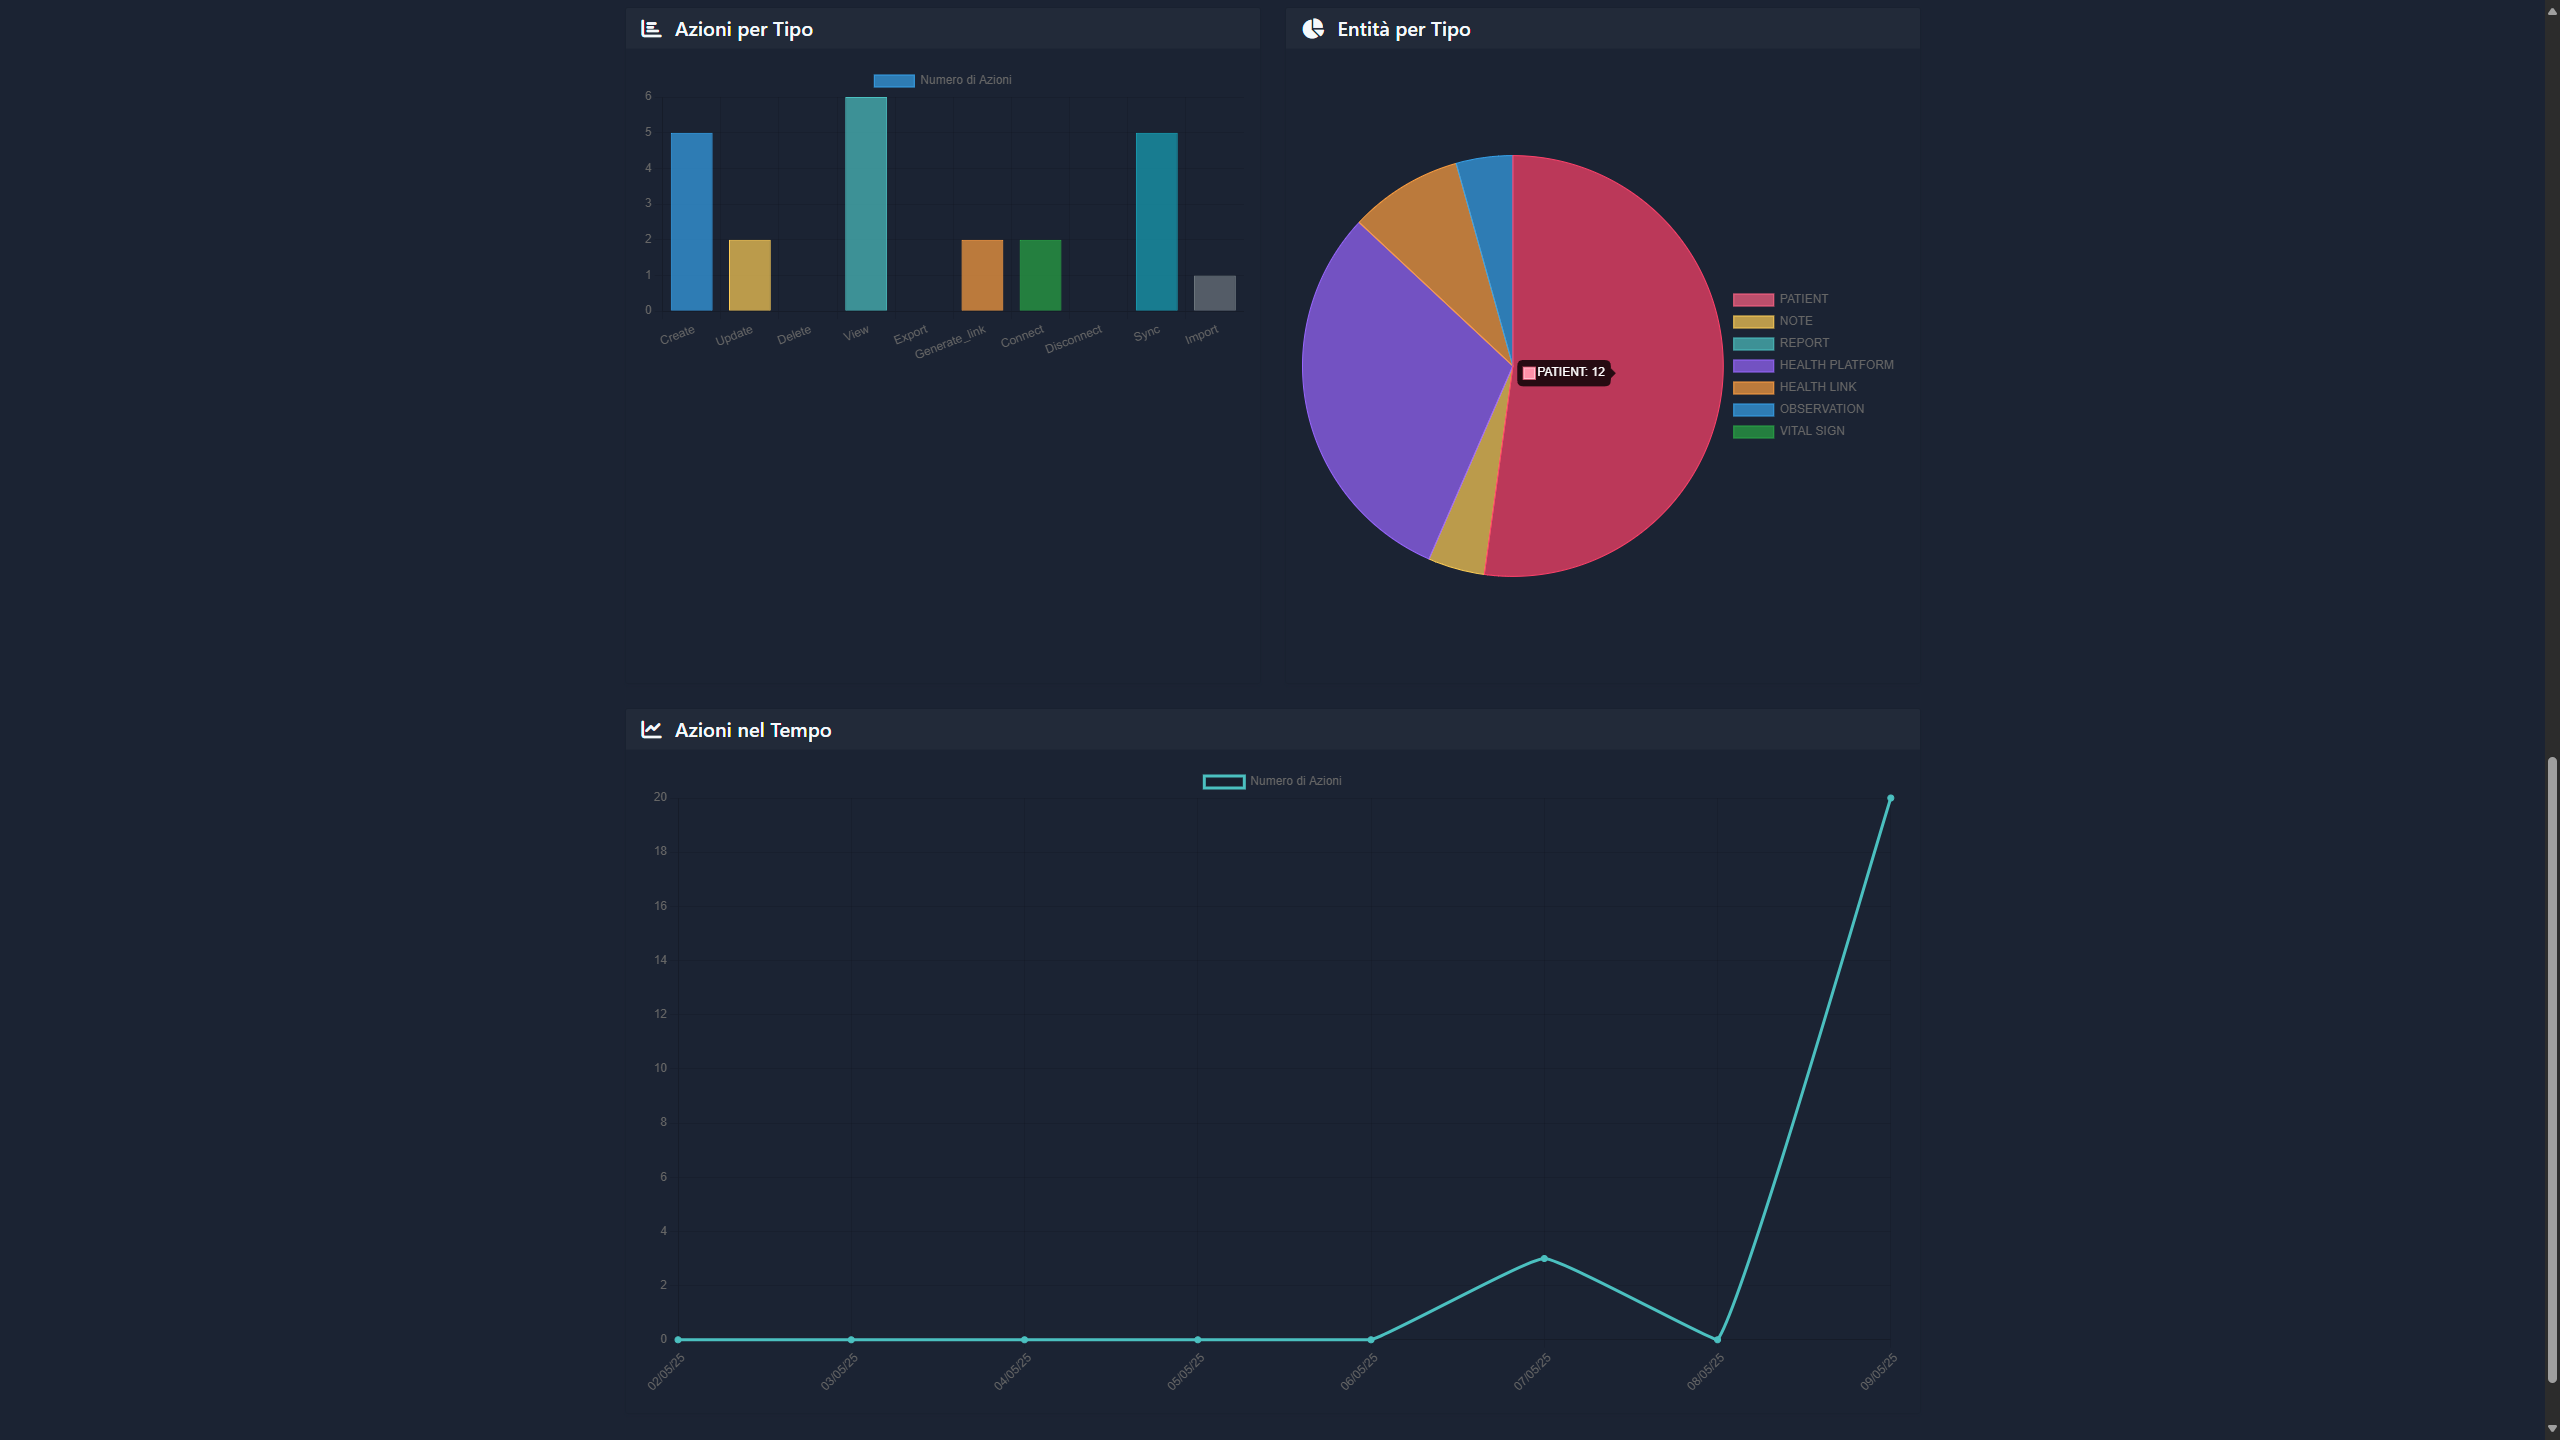
\includegraphics[width=0.85\textwidth]{images/screen/audit graph.png}
    \caption{Grafici di audit: visualizzazione grafica delle attività di audit per un'analisi statistica delle operazioni effettuate}
    \label{fig:audit-graph}
\end{figure}

\subsection{Endpoints}

L'applicazione espone numerosi endpoint sia per l'interfaccia web che per le API REST. Qui sotto sono elencati i principali endpoint organizzati per categoria, con la relativa descrizione, modulo di implementazione e parametri.

\subsubsection{Autenticazione}

\paragraph{Registrazione Medico}
\begin{itemize}
    \item \textbf{GET \texttt{/register}}
          \begin{itemize}
              \item \textbf{Modulo}: \texttt{app/auth.py}
              \item \textbf{Descrizione}: Mostra il modulo di registrazione per i nuovi medici.
              \item \textbf{Autenticazione}: Non richiesta
              \item \textbf{Risposta}: Form HTML per la registrazione di un nuovo account medico.
          \end{itemize}

    \item \textbf{POST \texttt{/register}}
          \begin{itemize}
              \item \textbf{Modulo}: \texttt{app/auth.py}
              \item \textbf{Descrizione}: Elabora il modulo di registrazione e crea un nuovo account medico.
              \item \textbf{Parametri}:
                    \begin{itemize}
                        \item \texttt{email}: Indirizzo email del medico (deve essere univoco)
                        \item \texttt{first\_name}: Nome del medico
                        \item \texttt{last\_name}: Cognome del medico
                        \item \texttt{specialty}: Specializzazione medica
                        \item \texttt{password}: Password (deve soddisfare i requisiti di sicurezza)
                        \item \texttt{confirm\_password}: Conferma della password
                    \end{itemize}
              \item \textbf{Risposta}: Reindirizzamento alla pagina di login in caso di successo, altrimenti visualizzazione del modulo con messaggi di errore.
          \end{itemize}
\end{itemize}

\paragraph{Login Medico}
\begin{itemize}
    \item \textbf{GET \texttt{/login}}
          \begin{itemize}
              \item \textbf{Modulo}: \texttt{app/auth.py}
              \item \textbf{Descrizione}: Mostra il modulo di login per i medici.
              \item \textbf{Autenticazione}: Non richiesta
              \item \textbf{Risposta}: Form HTML per il login.
          \end{itemize}

    \item \textbf{POST \texttt{/login}}
          \begin{itemize}
              \item \textbf{Modulo}: \texttt{app/auth.py}
              \item \textbf{Descrizione}: Autentica un medico e stabilisce una sessione.
              \item \textbf{Parametri}:
                    \begin{itemize}
                        \item \texttt{email}: Indirizzo email del medico
                        \item \texttt{password}: Password dell'account medico
                    \end{itemize}
              \item \textbf{Risposta}: Reindirizzamento alla dashboard in caso di successo, altrimenti visualizzazione del modulo di login con messaggi di errore.
          \end{itemize}
\end{itemize}

\paragraph{Logout Medico}
\begin{itemize}
    \item \textbf{GET \texttt{/logout}}
          \begin{itemize}
              \item \textbf{Modulo}: \texttt{app/auth.py}
              \item \textbf{Descrizione}: Termina la sessione autenticata del medico.
              \item \textbf{Autenticazione}: Richiesta
              \item \textbf{Risposta}: Reindirizzamento alla pagina di login con messaggio di conferma.
          \end{itemize}
\end{itemize}

\paragraph{API Login}
\begin{itemize}
    \item \textbf{POST \texttt{/api/login}}
          \begin{itemize}
              \item \textbf{Modulo}: \texttt{app/auth.py}
              \item \textbf{Descrizione}: Endpoint API per l'autenticazione dei medici. Valida le credenziali e genera token JWT per l'accesso alle API.
              \item \textbf{Tipo di Contenuto}: JSON
              \item \textbf{Parametri}:
                    \begin{verbatim}
{
  "email": "medico@esempio.com",
  "password": "password_sicura"
}
        \end{verbatim}
              \item \textbf{Risposta di Successo} (200 OK):
                    \begin{verbatim}
{
  "message": "Login effettuato con successo",
  "doctor": {
    "id": 1,
    "first_name": "Mario",
    "last_name": "Rossi",
    "email": "medico@esempio.com",
    "specialty": "Cardiologia"
  },
  "access_token": "eyJhbGciOiJIUz...",
  "refresh_token": "eyJhbGciOiJIUz..."
}
        \end{verbatim}
              \item \textbf{Possibili Errori}:
                    \begin{itemize}
                        \item 400 Bad Request: Richiesta JSON mancante o credenziali incomplete
                        \item 401 Unauthorized: Credenziali non valide
                    \end{itemize}
          \end{itemize}
\end{itemize}

\subsubsection{Gestione Pazienti}

\paragraph{Elenco Pazienti}
\begin{itemize}
    \item \textbf{GET \texttt{/api/patients}}
          \begin{itemize}
              \item \textbf{Modulo}: \texttt{app/api.py}
              \item \textbf{Descrizione}: Recupera l'elenco di tutti i pazienti associati al medico autenticato.
              \item \textbf{Autenticazione}: JWT richiesto
              \item \textbf{Risposta di Successo} (200 OK):
                    \begin{verbatim}
{
  "patients": [
    {
      "id": 1,
      "uuid": "123e4567-e89b-12d3-a456",
      "first_name": "Giovanni",
      "last_name": "Bianchi",
      "date_of_birth": "1980-05-15",
      "gender": "male",
      "contact_info": "telefono: +39 123456789",
      "created_at": "2023-05-01T14:30:00Z"
    },
    ...altri pazienti...
  ]
}
        \end{verbatim}
          \end{itemize}
\end{itemize}

\paragraph{Dettagli Paziente}
\begin{itemize}
    \item \textbf{GET \texttt{/api/patients/<string:patient\_uuid>}}
          \begin{itemize}
              \item \textbf{Modulo}: \texttt{app/api.py}
              \item \textbf{Descrizione}: Ottiene informazioni dettagliate su un paziente specifico.
              \item \textbf{Autenticazione}: JWT richiesto
              \item \textbf{Parametri URL}: \texttt{patient\_uuid} - UUID univoco del paziente
              \item \textbf{Risposta di Successo} (200 OK):
                    \begin{spverbatim}
                        {
                        "patient": {
                        "id": 1,
                        "uuid": "123e4567-e89b-12d3-a456",
                        "first_name": "Giovanni",
                        "last_name": "Bianchi",
                        "date_of_birth": "1980-05-15",
                        "gender": "male",
                        "contact_info": "telefono: +39 123456789",
                        "medical_history": "Ipertensione, allergia agli arachidi",
                        "created_at": "2023-05-01T14:30:00Z"
                        }
                        }
                    \end{spverbatim}
              \item \textbf{Possibili Errori}:
                    \begin{itemize}
                        \item 400 Bad Request: Formato UUID non valido
                        \item 403 Forbidden: Medico non autorizzato ad accedere a questo paziente
                        \item 404 Not Found: Paziente non trovato
                    \end{itemize}
          \end{itemize}
\end{itemize}

\paragraph{Parametri Vitali del Paziente}
\begin{itemize}
    \item \textbf{GET \texttt{/api/patients/<string:patient\_uuid>/vitals}}
          \begin{itemize}
              \item \textbf{Modulo}: \texttt{app/api.py}
              \item \textbf{Descrizione}: Recupera i parametri vitali di un paziente dalla piattaforma sanitaria collegata (ad es. Fitbit).
              \item \textbf{Autenticazione}: JWT richiesto
              \item \textbf{Parametri URL}: \texttt{patient\_uuid} - UUID univoco del paziente
              \item \textbf{Parametri Query}:
                    \begin{itemize}
                        \item \texttt{type} (opzionale): Tipo di segno vitale da recuperare (es. 'heart\_rate', 'steps')
                        \item \texttt{start\_date} (opzionale): Data di inizio per il range di dati in formato ISO (YYYY-MM-DD)
                        \item \texttt{end\_date} (opzionale): Data di fine per il range di dati in formato ISO (YYYY-MM-DD)
                    \end{itemize}
              \item \textbf{Risposta di Successo} (200 OK, esempio per type='heart\_rate'):
                    \begin{verbatim}
{
  "heart_rate": [
    {
      "timestamp": "2023-05-01T14:30:00Z",
      "value": 72,
      "unit": "bpm"
    },
    ...altri dati di frequenza cardiaca...
  ]
}
        \end{verbatim}
          \end{itemize}
\end{itemize}

\subsubsection{Note Mediche}

\paragraph{Elenco Note}
\begin{itemize}
    \item \textbf{GET \texttt{/api/patients/<string:patient\_uuid>/notes}}
          \begin{itemize}
              \item \textbf{Modulo}: \texttt{app/api.py}
              \item \textbf{Descrizione}: Recupera tutte le note mediche associate ad un paziente specifico.
              \item \textbf{Autenticazione}: JWT richiesto
              \item \textbf{Parametri URL}: \texttt{patient\_uuid} - UUID univoco del paziente
              \item \textbf{Risposta di Successo} (200 OK):
                    \begin{spverbatim}
                        {
                        "notes": [
                        {
                                "id": 1,
                                "content": "Il paziente ha riportato un miglioramento dei sintomi",
                                "doctor_id": 2,
                                "doctor_name": "Dott.ssa Laura Verdi",
                                "created_at": "2023-05-01T14:30:00Z"
                            },
                        ...altre note...
                        ]
                        }
                    \end{spverbatim}
          \end{itemize}
\end{itemize}

\paragraph{Aggiunta Nota}
\begin{itemize}
    \item \textbf{POST \texttt{/api/patients/<string:patient\_uuid>/notes}}
          \begin{itemize}
              \item \textbf{Modulo}: \texttt{app/api.py}
              \item \textbf{Descrizione}: Aggiunge una nuova nota medica per un paziente specifico.
              \item \textbf{Autenticazione}: JWT richiesto
              \item \textbf{Parametri URL}: \texttt{patient\_uuid} - UUID univoco del paziente
              \item \textbf{Corpo Richiesta}:
                    \begin{spverbatim}
                        {
                            "content": "Il paziente ha riportato un miglioramento dei sintomi dopo il cambio di terapia."
                        }
                    \end{spverbatim}
              \item \textbf{Risposta di Successo} (201 Created):
                    \begin{spverbatim}
                        {
                        "message": "Nota aggiunta con successo",
                        "note": {
                        "id": 2,
                        "content": "Il paziente ha riportato un miglioramento dei sintomi dopo il cambio di terapia.",
                        "doctor_id": 2,
                        "doctor_name": "Dott.ssa Laura Verdi",
                        "created_at": "2023-05-10T09:15:00Z"
                        }
                        }
                    \end{spverbatim}
          \end{itemize}
\end{itemize}

\subsubsection{Osservazioni dei Parametri Vitali}

\paragraph{Elenco Osservazioni}
\begin{itemize}
    \item \textbf{GET \texttt{/api/patients/<int:patient\_id>/observations}}
          \begin{itemize}
              \item \textbf{Modulo}: \texttt{app/api.py}
              \item \textbf{Descrizione}: Recupera le osservazioni sui parametri vitali per un paziente specifico.
              \item \textbf{Autenticazione}: JWT richiesto
              \item \textbf{Parametri URL}: \texttt{patient\_id} - ID del paziente
              \item \textbf{Parametri Query}:
                    \begin{itemize}
                        \item \texttt{start\_date} (opzionale): Data di inizio per filtrare le osservazioni in formato ISO
                        \item \texttt{end\_date} (opzionale): Data di fine per filtrare le osservazioni in formato ISO
                        \item \texttt{vital\_type} (opzionale): Tipo di segno vitale per filtrare le osservazioni
                    \end{itemize}
          \end{itemize}
\end{itemize}

\subsubsection{Piattaforme Sanitarie}

\paragraph{Connessione Piattaforma}
\begin{itemize}
    \item \textbf{POST \texttt{/health-platforms/connect/<string:platform\_name>}}
          \begin{itemize}
              \item \textbf{Modulo}: \texttt{app/health\_platforms.py}
              \item \textbf{Descrizione}: Connette un paziente a una piattaforma sanitaria esterna (es. Fitbit).
              \item \textbf{Autenticazione}: JWT richiesto
              \item \textbf{Parametri URL}: \texttt{platform\_name} - Nome della piattaforma sanitaria (es. 'fitbit')
              \item \textbf{Corpo Richiesta}:
                    \begin{verbatim}
{
  "patient_id": 1,
  "access_token": "oauth-access-token",
  "refresh_token": "oauth-refresh-token",
  "expires_at": "2024-05-01T00:00:00Z"
}
        \end{verbatim}
          \end{itemize}
\end{itemize}

\paragraph{Dati Fitbit}
\begin{itemize}
    \item \textbf{GET \texttt{/health-platforms/fitbit/<string:patient\_uuid>}}
          \begin{itemize}
              \item \textbf{Modulo}: \texttt{app/health\_platforms.py}
              \item \textbf{Descrizione}: Recupera i dati Fitbit per un paziente specifico.
              \item \textbf{Autenticazione}: JWT richiesto
              \item \textbf{Parametri URL}: \texttt{patient\_uuid} - UUID del paziente
              \item \textbf{Parametri Query}:
                    \begin{itemize}
                        \item \texttt{type} (opzionale): Tipo di dati Fitbit da recuperare (es. 'heart\_rate', 'sleep')
                        \item \texttt{start\_date} (opzionale): Data di inizio in formato ISO
                        \item \texttt{end\_date} (opzionale): Data di fine in formato ISO
                    \end{itemize}
          \end{itemize}
\end{itemize}

\subsubsection{Gestione Interfaccia Web}

\paragraph{Dashboard}
\begin{itemize}
    \item \textbf{GET \texttt{/dashboard}}
          \begin{itemize}
              \item \textbf{Modulo}: \texttt{app/views.py}
              \item \textbf{Descrizione}: Visualizza la dashboard principale del medico con panoramica dei pazienti, attività recenti e statistiche.
              \item \textbf{Autenticazione}: Login richiesto
              \item \textbf{Risposta}: Pagina HTML della dashboard.
          \end{itemize}
\end{itemize}

\paragraph{Elenco Pazienti}
\begin{itemize}
    \item \textbf{GET \texttt{/patients}}
          \begin{itemize}
              \item \textbf{Modulo}: \texttt{app/views.py}
              \item \textbf{Descrizione}: Mostra l'elenco di tutti i pazienti associati al medico autenticato.
              \item \textbf{Autenticazione}: Login richiesto
              \item \textbf{Risposta}: Pagina HTML con l'elenco dei pazienti.
          \end{itemize}
\end{itemize}

\paragraph{Nuovo Paziente}
\begin{itemize}
    \item \textbf{GET \texttt{/patients/new}}
          \begin{itemize}
              \item \textbf{Modulo}: \texttt{app/views.py}
              \item \textbf{Descrizione}: Mostra il modulo per la creazione di un nuovo paziente.
              \item \textbf{Autenticazione}: Login richiesto
              \item \textbf{Risposta}: Pagina HTML con il form per la creazione del paziente.
          \end{itemize}

    \item \textbf{POST \texttt{/patients/new}}
          \begin{itemize}
              \item \textbf{Modulo}: \texttt{app/views.py}
              \item \textbf{Descrizione}: Processa il modulo di creazione paziente e crea un nuovo record paziente.
              \item \textbf{Autenticazione}: Login richiesto
              \item \textbf{Parametri}:
                    \begin{itemize}
                        \item \texttt{first\_name}: Nome del paziente
                        \item \texttt{last\_name}: Cognome del paziente
                        \item \texttt{date\_of\_birth}: Data di nascita
                        \item \texttt{gender}: Genere
                        \item \texttt{contact\_info}: Informazioni di contatto
                        \item \texttt{medical\_history}: Storia clinica (opzionale)
                    \end{itemize}
          \end{itemize}
\end{itemize}

\paragraph{Report}
\begin{itemize}
    \item \textbf{GET \texttt{/reports}}
          \begin{itemize}
              \item \textbf{Modulo}: \texttt{app/views.py}
              \item \textbf{Descrizione}: Mostra la pagina per la generazione di report.
              \item \textbf{Autenticazione}: Login richiesto
              \item \textbf{Risposta}: Pagina HTML con opzioni per la generazione di report.
          \end{itemize}

    \item \textbf{POST \texttt{/reports}}
          \begin{itemize}
              \item \textbf{Modulo}: \texttt{app/views.py}
              \item \textbf{Descrizione}: Genera e scarica un report basato sui parametri specificati.
              \item \textbf{Autenticazione}: Login richiesto
              \item \textbf{Parametri Form}:
                    \begin{itemize}
                        \item \texttt{report\_type}: Tipo di report da generare
                        \item \texttt{start\_date}: Data di inizio del report
                        \item \texttt{end\_date}: Data di fine del report
                        \item \texttt{patient\_id} (opzionale): ID del paziente se il report è specifico per un paziente
                    \end{itemize}
              \item \textbf{Risposta}: File del report (PDF, CSV, ecc.) scaricabile o messaggio di errore.
          \end{itemize}
\end{itemize}

\subsubsection{Audit e Statistiche}

\paragraph{Log di Audit}
\begin{itemize}
    \item \textbf{GET \texttt{/audit/logs}}
          \begin{itemize}
              \item \textbf{Modulo}: \texttt{app/audit.py}
              \item \textbf{Descrizione}: Visualizza i log di audit con possibilità di filtraggio.
              \item \textbf{Autenticazione}: Login richiesto (solo per amministratori)
              \item \textbf{Parametri Query}:
                    \begin{itemize}
                        \item \texttt{start\_date} (opzionale): Data di inizio per il filtraggio
                        \item \texttt{end\_date} (opzionale): Data di fine per il filtraggio
                        \item \texttt{doctor\_id} (opzionale): ID del medico per filtrare le azioni
                        \item \texttt{action\_type} (opzionale): Tipo di azione da filtrare
                    \end{itemize}
          \end{itemize}
\end{itemize}

\paragraph{Statistiche}
\begin{itemize}
    \item \textbf{GET \texttt{/audit/stats}}
          \begin{itemize}
              \item \textbf{Modulo}: \texttt{app/audit.py}
              \item \textbf{Descrizione}: Visualizza le statistiche aggregate dell'uso del sistema.
              \item \textbf{Autenticazione}: Login richiesto (solo per amministratori)
              \item \textbf{Risposta}: Pagina HTML con grafici e tabelle statistiche.
          \end{itemize}
\end{itemize}

\paragraph{Cambio Lingua}
\begin{itemize}
    \item \textbf{GET \texttt{/lang/<string:lang\_code>}}
          \begin{itemize}
              \item \textbf{Modulo}: \texttt{app/language.py}
              \item \textbf{Descrizione}: Cambia la lingua dell'interfaccia utente.
              \item \textbf{Autenticazione}: Non richiesta
              \item \textbf{Parametri URL}: \texttt{lang\_code} - Codice della lingua (es. 'it', 'en')
              \item \textbf{Risposta}: Reindirizzamento alla pagina precedente con la nuova lingua impostata.
          \end{itemize}
\end{itemize}


\chapter{Testing e Validazione}
\section{Strategia di testing}
\subsection{Approccio al testing e ambiente}
Per il testing l'approccio ha previsto la configurazione dell'ambiente di test con un file .env.test specifico per l'ambiente di test.
Per eseguire i test infatti è necessario avere un database e, per evitare di compromettere l'integrità del database effettivo utilizzato in produzione, è stato creato un database in-memory SQLite che ha permesso di isolare le operazioni effettuate.
\subsection{Automazione dei test}
Per automatizzare i test, è stato utilizzato un framework di testing chiamato pytest \cite{pytest}.
\section{Unit testing}
Per ciascun modulo principale è stato scritto un set di test unitari per verificare il corretto funzionamento delle singole funzioni e che queste sddisfassero i requisiti specifici.
L'obiettivo principale che ha guidato questa fase è stato cercare di raggiungere la copertura maggiore possibile.
\subsection{Mock e fixture}
Le fixture in pytest rappresentano un metodo per fornire dati, oggetti o configurazioni necessarie ai test.
In VitaLink le fixture sono centralizzate nel file \texttt{conftest.py}, che costituisce il modulo cardine dell'infrastruttura di test.
\subsection{Analisi statica del codice}
Per l'analisi statica del codice si è deciso di utilizzare un workflow automatizzato Github Actions, in modo da poter ottenere un'analisi coerente con ciascun nuovo commit.
I risultati dei test sono consultabili sulla Page di Github del progetto, configurata per accogliere anche la documentazione del codice sorgente e dei tests.
Tale workflow include i seguenti strumenti per l'analisi:
\begin{itemize}
    \item \textbf{Pipdeptree}: Crea un albero delle dipendenze del progetto.

    \item \textbf{coverage}: Misura quanto del codice viene eseguito durante i test.

    \item \textbf{Radon}: Per l’analisi della complessità e manutenibilità del codice.

    \item \textbf{Cloc}: Conta linee di codice, commenti, e file.
\end{itemize}

\chapter{Deployment e Operations}
\section{Ambiente di deployment}
\subsection{Configurazione del server}
Un server di produzione è stato configurato per testare l'effettivo funzionamento della piattaforma nel caso di deployment in un ambiente reale.
Koyeb \cite{koyeb} ha permesso l'istanziazione di un database PostgreSQL, oltre che ad un server Gunicorn per l'esecuzione del backend.
\subsection{Gestione delle variabili d'ambiente}\sloppy
Le variabili d'ambiente sono state configurate con i dettagli dell'implementazione cloud, andando a settare le variabili \texttt{CLOUD\_RUN\_ENVIRONMENT=true}, oltre a \texttt{INSTANCE\_UNIX\_SOCKET, DB\_USER, DB\_PASS, DB\_NAME}
con i dettagli di accesso al database cloud e \texttt{FITBIT\_CLIENT\_ID, FITBIT\_CLIENT\_SECRET, FITBIT\_REDIRECT\_URI} con i dettagli di accesso alla piattaforma Fitbit e \texttt{MJ\_APIKEY, MJ\_APISECRET, EMAIL\_SENDER} per l'integrazione con Mailjet.
\section{Containerizzazione e orchestrazione}
\subsection{Docker e Docker Compose}
Docker e Docker Compose hanno rappresentato strumenti fondamentali per la containerizzazione dell'applicazione VitaLink, garantendo un ambiente di sviluppo e produzione coerente e riproducibile. Il file \texttt{docker-compose.yml} definisce due servizi principali: \texttt{web} per l'applicazione Flask e \texttt{db} per il database PostgreSQL. Il servizio \texttt{web} si basa sull'immagine costruita a partire dal Dockerfile e include configurazioni per dipendenze, porte e controlli di salute. Il servizio \texttt{db} utilizza l'immagine ufficiale \texttt{postgres:15-alpine}, ottimizzata per dimensioni ridotte e prestazioni. La configurazione integrata garantisce che il database sia disponibile prima dell'avvio dell'applicazione grazie alla direttiva \texttt{depends\_on}, facilitando l'orchestrazione dei container.

\subsection{Immagini e configurazione}
La configurazione delle immagini Docker è stata ottimizzata per garantire un ambiente di esecuzione leggero ma completo. L'immagine dell'applicazione web si basa su \texttt{python:3.11-slim}, che offre un buon compromesso tra dimensioni e funzionalità. Nel Dockerfile sono installati solo i pacchetti essenziali (\texttt{gcc}, \texttt{libpq-dev}, \texttt{postgresql-client}, ecc.) necessari per la compilazione delle dipendenze Python e l'interazione con PostgreSQL. La configurazione prevede inoltre l'utilizzo di Gunicorn come server WSGI con tre worker per ottimizzare le prestazioni. Il parametro \texttt{FLASK\_APP} viene impostato dinamicamente attraverso variabili d'ambiente, consentendo una maggiore flessibilità di configurazione tra ambienti diversi. Inoltre, gli script di inizializzazione \texttt{docker-entrypoint.sh} e \texttt{db\_migrate.sh} vengono eseguiti all'avvio del container per garantire la corretta configurazione e migrazione del database.

\subsection{Persistenza dei dati}
La persistenza dei dati è un aspetto cruciale in un'applicazione come VitaLink che gestisce informazioni sanitarie. La soluzione adottata si basa su volumi Docker, in particolare sul volume \texttt{postgres\_data} configurato nel \texttt{docker-compose.yml}, che viene mappato sulla directory interna di PostgreSQL \texttt{/var/lib/postgresql/data}. Questo approccio garantisce che i dati sopravvivano al riavvio dei container o alla ricostruzione dell'immagine, preservando l'integrità delle informazioni dei pazienti e delle loro misurazioni. La separazione tra container e dati permette anche di semplificare le procedure di backup, poiché è possibile eseguire backup del volume indipendentemente dallo stato dei container. Questa architettura supporta inoltre scenari di disaster recovery, consentendo di ripristinare rapidamente il sistema in caso di problemi hardware o software.

\section{Continuous Integration e Continuous Deployment}
\subsection{Pipeline CI/CD}
La pipeline di Continuous Integration e Continuous Deployment (CI/CD) di VitaLink è stata implementata utilizzando GitHub Actions, creando un processo automatizzato che accompagna il codice dalla fase di sviluppo fino al deployment. La pipeline è strutturata in diverse fasi: inizia con il checkout del codice sorgente, prosegue con la configurazione dell'ambiente Python, l'installazione delle dipendenze, l'esecuzione dei test e infine, per il ramo principale, il deployment automatico. Ogni fase è condizionata dal successo di quella precedente, garantendo che solo il codice che supera tutti i controlli di qualità raggiunga l'ambiente di produzione. Questa automazione ha ridotto significativamente il rischio di errori umani nel processo di rilascio e ha accelerato il ciclo di feedback, consentendo di identificare e risolvere i problemi più rapidamente.

\subsection{Automazione dei test}
L'automazione dei test rappresenta una componente fondamentale del workflow di CI/CD di VitaLink. Ad ogni commit o pull request, GitHub Actions esegue automaticamente la suite completa dei test per verificare che le modifiche non introducano regressioni. La configurazione prevede l'esecuzione di test unitari con pytest in un ambiente isolato, verifiche di qualità del codice con strumenti come Flake8 e Pylint, e analisi della copertura dei test con coverage. I risultati dei test vengono pubblicati direttamente nell'interfaccia di GitHub, fornendo feedback immediato agli sviluppatori. Inoltre, per i test che richiedono l'interazione con servizi esterni come l'API di Fitbit, sono stati implementati mock specifici per simulare le risposte, garantendo che i test siano deterministici e non dipendano dalla disponibilità di servizi esterni.

\subsection{Deployment automatizzato}
Il deployment automatizzato di VitaLink è configurato per attivarsi solo quando le modifiche vengono incorporate nel ramo principale (\texttt{main}) e tutti i test sono stati superati con successo. Il processo di deployment utilizza le credenziali sicure memorizzate come segreti di GitHub Actions e comprende diverse fasi: costruzione dell'immagine Docker, push al Container Registry, e deployment sull'infrastruttura cloud. La configurazione include anche meccanismi di rollback automatico in caso di problemi durante il deployment, garantendo la continuità del servizio. Un aspetto particolarmente importante è l'applicazione delle migrazioni del database, che viene gestita dallo script \texttt{db\_migrate.sh} durante l'avvio del container, assicurando che lo schema del database sia sempre sincronizzato con il codice dell'applicazione. Questo approccio garantisce deployment frequenti e sicuri, abilitando un modello di sviluppo realmente continuo.

\section{Logging}
\subsection{Strategia di logging}
Per il backend della piattaforma è stato implementato un sistema di logging estensivo per monitorare le attività e gli errori.

\subsection{Gestione degli errori}
La strategia in caso di errore ha previsto la registrazione di un messaggio dettagliato in console, includendo anche i dettagli dell'eccezione.
Nel caso di errori critici, il workflow configurato su Github Actions ha permesso di identificare quasi istantaneamente e risolvere i problemi.

\chapter{Risultati e valutazione}
\section{Obiettivi raggiunti}
\subsection{Funzionalità implementate}
Il risultato finale dell'implementazione della piattaforma VitaLink prevedere l'integrazione di tutte le funzionalità di base descritte nei requisiti iniziali.
La struttura modulare del codice ha permesso di aggiungere funzionalità aggiuntive anche in fase di testing e deployment, qualora ciò si si fosse reso necessario.

\section{Limiti e problemi riscontrati}
\subsection{Sfide tecniche}
La più grande limitazione tecnica è stata rappresentata in primis dalle API esterne, le quali (come nel caso di Fitbit) richiedono un server di callback in formato HTTPS.
Ciò ha richiesto l'utilizzo di un server di produzione configurato opportunamente anche in fase di testing, andando a complicare leggermente il processo di sviluppo.
Un altro problema è stato rappresentato dalla difficoltà di trovare un servizio di hosting gratuito che permettesse l'uso di tutti i componenti richiesti (database relazionale, server WSGI, ecc.), il che ha richiesto un compromesso tra costi e funzionalità (la scalabilità del servizio risulta infatti limitata ad un'istanza nel caso di utilizzo di Koyeb con la prova gratuita).
\subsection{Limitazioni delle API esterne}
Le API esterne di Fitbit, come indicato sul sito di PublicAPI \cite{fitbit_API_rate}, presentano un rate limit piuttosto basso (150 richieste all'ora). Tale limite ha imposto un ritmo di sviluppo più lento in quanto per ciascuna funzionalità implementata, il testing correlato richiedeva delle richieste API che andavano molto rapidamente a depletare il limite orario (richiedendo quindi di creare vari account di test Fitbit per aggirare tale limite).

\chapter{Conclusioni e sviluppi futuri}
\section{Conclusioni}
\subsection{Contributi principali}
Tutto il lavoro è stato svolto in autonomia, dalla progettazione iniziale fino al deployment della piattaforma.
Tutte le fonti utilizzate per per l'apprendimento e la realizzazione del progetto sono state debitamente citate.

\subsection{Riflessione sul processo di sviluppo}
Il processo di sviluppo ha seguito un approccio aderente ai principi imparati durante il corso di Ingegneria del Software, con particolare attenzione alla fase di progettazione e alla scrittura di codice manutenibile e testabile.
L'adozione delle pratiche di CI/CD ha permesso di automatizzare alcune delle operazioni ripetitive e di ridurre il rischio di errore umano.

\section{Sviluppi futuri}
\subsection{Integrazione con ulteriori piattaforme sanitarie}
Per il momento non si prevede l'integrazione con ulteriori piattaforme sanitarie. Ciò nonostante, la modularità del codice permette di aggiungere facilmente nuovi moduli per l'integrazione con altre piattaforme che supportino OAuth 2.0 e dispongano di API REST.
Il progetto verrà mantenuto sul repository GitHub a tempo indefinito, in modo da permettere a chiunque di contribuire allo sviluppo futuro, oltre che a poter consultare il repository in qualunque momento.

\subsection{Applicazione mobile companion}
Per il futuro si potrebbe pensare di sviluppare un'applicazione mobile companion per il personale sanitario, in maniera tale da permettere l'accesso alle funzionalità principali direttamente dal proprio smartphone.
Tale applicazione non richiederebbe sostanziali modifiche al backend in quanto sono già implementante API REST utilizzabili a tal fine. Potrebbe essere invece pensabile l'implementazione di ulteriori API REST per richieste più fine-grained, in modo da ridurre il carico di dati trasferiti.
\section{Considerazioni personali}
\subsection{Sfide personali}
La conciliazione tra lavoro nel fine settimana, studio per completare gli ultimi esami e lo sviluppo del progetto ha rappresentato una sfida non indifferente.
Per riuscire a portare avanti tutte le attività sopra citate, è stata necessaria un'attenta pianificazione, oltre che a una buona dose di sacrificio personale.
\subsection{Valore aggiunto dell'esperienza}
Il valore aggiunto di questa esperienza è stato rappresentato dalla possibilità di mettere in pratica le conoscenze acquisite durante il corso di Ingegneria del Software, oltre che di apprendere nuove tecnologie e metodologie di sviluppo.
La più grande quantità di informazioni appresa è stata quella relativa al framework Flask, il quale mi tornerà sicuramente utile in futuro nel mondo lavorativo.
% Appendici
\appendix

\chapter{Glossario}
\begin{description}
    \item[API] Application Programming Interface
    \item[Bootstrap] Framework CSS per lo sviluppo di interfacce web responsive e moderne
    \item[CI/CD] Continuous Integration/Continuous Deployment
    \item[CRUD] Create, Read, Update, Delete - Le quattro operazioni fondamentali su dati persistenti
    \item[DBMS] Database Management System - Sistema software per la gestione di basi di dati
    \item[Flask] Framework web leggero per Python utilizzato per lo sviluppo di applicazioni web
    \item[Gunicorn] Green Unicorn, server WSGI HTTP per applicazioni Python
    \item[JWT] JSON Web Token
    \item[MVC] Model-View-Controller
    \item[OAuth 2.0] Protocollo di autorizzazione standard dell'industria
    \item[ORM] Object-Relational Mapping
    \item[PostgreSQL] Sistema di gestione di database relazionali open source
    \item[Rate Limit] Limitazione del numero di richieste API in un determinato periodo di tempo
    \item[REST] Representational State Transfer
    \item[SQLAlchemy] Toolkit SQL e ORM per Python
    \item[TTL] Time-to-Live - Periodo di validità di un dato in cache
    \item[UI] User Interface
    \item[UML] Unified Modeling Language
    \item[UUID] Universally Unique Identifier
    \item[WSGI] Web Server Gateway Interface - Specifica per interfacce tra server web e applicazioni Python
\end{description}

\chapter{Diagrammi UML}
Alcuni diagrammi UML risultano eccessivamente complessi per essere riportati in forma di immagine. Viene fornito il codice PlantUML per la generazione dei diagrammi, i quali potranno essere visualizzati tramite l'estensione di VS Code \cite{plantvscode} oppure tramite il sito di PlantUML \cite{plantuml}.
\section{Diagrammi dei casi d'uso}
\begin{lstlisting}[basicstyle=\small\ttfamily, breaklines=true]
@startuml "DiagrammaCasiDUso"

' Use Case Diagram for VitaLink application
title Diagramma dei Casi d'Uso - VitaLink

' Style parameters
skinparam actorStyle awesome
skinparam shadowing false
skinparam packageStyle rectangle

left to right direction

' Actors
actor "Medico" as Doctor
actor "Paziente" as Patient
actor "Piattaforma Sanitaria" as HealthPlatform

' Use cases groups
rectangle "Sistema VitaLink" {
    ' Authentication
    rectangle "Gestione Account" {
        usecase "Registrazione" as UC1
        usecase "Login" as UC2
        usecase "Logout" as UC3
    }
    
    ' Dashboard
    rectangle "Dashboard" {
        usecase "Visualizzare Dashboard" as UC4
    }
    
    ' Audit
    rectangle "Gestione Audit" {
        usecase "Visualizzare Log di Audit" as UC5
        usecase "Visualizzare Dettagli Audit" as UC6
        usecase "Filtrare Audit" as UC7
    }
    
    ' Patient management
    rectangle "Gestione Pazienti" {
        usecase "Visualizzare Pazienti" as UC8
        usecase "Creare Nuovo Paziente" as UC9
        usecase "Importare Paziente tramite UUID" as UC10
        usecase "Visualizzare Dettagli Paziente" as UC11
        usecase "Modificare Paziente" as UC12
    }
    
    ' Notes
    rectangle "Gestione Note" {
        usecase "Aggiungere Nota" as UC13
        usecase "Visualizzare Note" as UC14
        usecase "Eliminare Nota" as UC15
    }
    
    ' Health platform integration
    rectangle "Integrazione Piattaforme Salute" {
        usecase "Generare Link per Connessione" as UC16
        usecase "Connettere Dispositivo" as UC17
        usecase "Disconnettere Dispositivo" as UC18
        usecase "Visualizzare Parametri Vitali" as UC19
    }
    
    ' Vital observations
    rectangle "Gestione Osservazioni" {
        usecase "Aggiungere Osservazione" as UC20
        usecase "Visualizzare Osservazioni" as UC21
        usecase "Eliminare Osservazione" as UC22
    }
    
    ' Reports
    rectangle "Gestione Report" {
        usecase "Generare Report Generale" as UC23
        usecase "Generare Report Specifico" as UC24
        usecase "Selezionare Elementi da Includere" as UC25
        usecase "Inviare Report per Email" as UC26
    }
    
    ' Data visualization
    rectangle "Visualizzazione Dati" {
        usecase "Visualizzare Grafici Parametri Vitali" as UC27
        usecase "Visualizzare Dati in Formato Tabellare" as UC28
        usecase "Selezionare Intervallo Temporale (1g, 7g, 1m, 3m)" as UC29
    }
}

' Relationships
Doctor --> UC1
Doctor --> UC2
Doctor --> UC3
Doctor --> UC4
Doctor --> UC5
Doctor --> UC6
Doctor --> UC7
Doctor --> UC8
Doctor --> UC9
Doctor --> UC10
Doctor --> UC11
Doctor --> UC12
Doctor --> UC13
Doctor --> UC14
Doctor --> UC15
Doctor --> UC16
Doctor --> UC17
Doctor --> UC18
Doctor --> UC19
Doctor --> UC20
Doctor --> UC21
Doctor --> UC22
Doctor --> UC23
Doctor --> UC24
Doctor --> UC25
Doctor --> UC26
Doctor --> UC27
Doctor --> UC28
Doctor --> UC29

' Extend/Include relationships
UC11 <.. UC13 : <<include>>
UC11 <.. UC14 : <<include>>
UC11 <.. UC15 : <<include>>
UC11 <.. UC16 : <<include>>
UC11 <.. UC19 : <<include>>
UC19 <.. UC20 : <<include>>
UC19 <.. UC21 : <<include>>
UC19 <.. UC22 : <<include>>
UC19 <.. UC27 : <<include>>
UC19 <.. UC28 : <<include>>
UC27 <.. UC29 : <<include>>
UC23 <.. UC25 : <<include>>
UC23 <.. UC26 : <<include>>
UC24 <.. UC25 : <<include>>
UC24 <.. UC26 : <<include>>

' Relazioni aggiuntive per altri attori
Patient --> UC17 : Autorizza connessione
HealthPlatform --> UC18 : Fornisce dati

' Note informative
note "Il sistema VitaLink permette ai medici di gestire i pazienti\ne monitorare i loro parametri vitali." as N1

note right of UC17
  Il paziente autorizza VitaLink ad accedere
  ai propri dati sulla piattaforma sanitaria
  tramite OAuth 2.0
end note

note right of UC4
  La dashboard mostra un riepilogo dei pazienti,
  attivita recenti e statistiche
end note

note right of UC5
  I log di audit permettono di tracciare
  tutte le azioni eseguite nel sistema
end note

@enduml

\end{lstlisting}
\section{Diagrammi delle classi}
\begin{lstlisting}[basicstyle=\small\ttfamily, breaklines=true]
@startuml "DiagrammaClassiCompleto"

' Class Diagram for VitaLink application
title Diagramma delle Classi Completo - VitaLink

' Packages to organize classes
package "Core & Configuration" {
    ' Base Classes
    abstract class Base {
    }
    
    class ApplicationConfig << (S,lightblue) >> {
        -debug: Boolean
        -host: String
        -port: Integer
        -sqlalchemy_database_uri: String
        -sqlalchemy_track_modifications: Boolean
        -jwt_secret_key: String
        -babel_default_locale: String
        -languages: Dictionary
    }
    
    class FlaskApp << (S,lightblue) >> {
        +secret_key: String
        +config: ApplicationConfig
        +run(): void
    }
}

package "Authentication" {
    ' Forms and User Management
    class RegistrationForm {
        +email: EmailField
        +first_name: StringField
        +last_name: StringField
        +specialty: StringField
        +password: PasswordField
        +confirm_password: PasswordField
        +validate(): Boolean
    }
    
    ' Flask-Login integration
    class UserMixin {
        +is_authenticated(): Boolean
        +is_active(): Boolean
        +is_anonymous(): Boolean
        +get_id(): String
    }
    
    ' Decorators 
    class AuthDecorators << (D,orchid) >> {
        +login_required(fn): Function
        +doctor_required(fn): Function
        +api_doctor_required(fn): Function
    }
}

package "Data Models" {
    ' Enums
    enum VitalSignType {
        +HEART_RATE
        +OXYGEN_SATURATION
        +BREATHING_RATE
        +WEIGHT
        +TEMPERATURE_CORE
        +TEMPERATURE_SKIN
        +STEPS
        +CALORIES
        +DISTANCE
        +ACTIVE_MINUTES
        +SLEEP_DURATION
        +FLOORS_CLIMBED
        +ELEVATION
        +ACTIVITY_CALORIES
        +CALORIES_BMR
        +MINUTES_SEDENTARY
        +MINUTES_LIGHTLY_ACTIVE
        +MINUTES_FAIRLY_ACTIVE
        +CALORIES_IN
        +WATER
    }

    enum HealthPlatform {
        +FITBIT
        +GOOGLE_HEALTH_CONNECT
        +APPLE_HEALTH
    }

    enum ActionType {
        +CREATE
        +UPDATE
        +DELETE
        +VIEW
        +EXPORT
        +GENERATE_LINK
        +CONNECT
        +DISCONNECT
        +SYNC
        +IMPORT
    }

    enum EntityType {
        +PATIENT
        +VITAL_SIGN
        +NOTE
        +REPORT
        +HEALTH_PLATFORM
        +HEALTH_LINK
        +OBSERVATION
    }

    ' Main Classes
    class Doctor {
        +id: Integer [PK]
        +email: String
        +password_hash: String
        +first_name: String
        +last_name: String
        +specialty: String
        +created_at: DateTime
        +updated_at: DateTime
        --
        +set_password(password: String): void
        +check_password(password: String): Boolean
        +to_dict(): Dictionary
        +get_patients(): List<Patient>
        +add_patient(patient: Patient): void
        +remove_patient(patient: Patient): void
    }

    class Patient {
        +id: Integer [PK]
        +uuid: String
        +first_name: String
        +last_name: String
        +date_of_birth: Date
        +gender: String
        +contact_number: String
        +email: String
        +address: Text
        +created_at: DateTime
        +updated_at: DateTime
        +connected_platform: HealthPlatform
        +platform_access_token: String
        +platform_refresh_token: String
        +platform_token_expires_at: DateTime
        --
        +to_dict(): Dictionary
        +get_vital_observations(vital_type: VitalSignType, start_date: DateTime, end_date: DateTime): List
        +get_notes(): List<Note>
    }

    class DoctorPatient {
        +doctor_id: Integer [PK, FK]
        +patient_id: Integer [PK, FK]
        +assigned_date: DateTime
    }

    class Note {
        +id: Integer [PK]
        +patient_id: Integer [FK]
        +doctor_id: Integer [FK]
        +content: Text
        +created_at: DateTime
        +updated_at: DateTime
        --
        +to_dict(): Dictionary
    }

    class VitalObservation {
        +id: Integer [PK]
        +patient_id: Integer [FK]
        +doctor_id: Integer [FK]
        +vital_type: VitalSignType
        +content: Text
        +start_date: DateTime
        +end_date: DateTime
        +created_at: DateTime
        +updated_at: DateTime
        --
        +to_dict(): Dictionary
    }

    class AuditLog {
        +id: Integer [PK]
        +doctor_id: Integer [FK]
        +timestamp: DateTime
        +action_type: ActionType
        +entity_type: EntityType
        +entity_id: Integer
        +details: Text
        +patient_id: Integer [FK]
        +ip_address: String
        --
        +__init__(doctor_id, action_type, entity_type, entity_id, details, patient_id, ip_address)
        +get_details(): Dictionary
        +to_dict(): Dictionary
    }

    class HealthPlatformLink {
        +id: Integer [PK]
        +uuid: String
        +patient_id: Integer [FK]
        +doctor_id: Integer [FK]
        +created_at: DateTime
        +expires_at: DateTime
        +used: Boolean
        +platform: HealthPlatform
        --
        +is_expired(): Boolean
        +to_dict(): Dictionary
    }
}

package "Service Modules" {
    class ObservationsService << (S,lightblue) >> {
        +get_web_observations(patient_id): List
        +add_web_observation(): VitalObservation
        +update_web_observation(observation_id): VitalObservation
        +delete_web_observation(observation_id): void
    }

    class HealthPlatformsService << (S,lightblue) >> {
        +vitals_cache: Dictionary
        +api_rate_limit: Dictionary
        --
        +generate_platform_link(patient_id, platform): HealthPlatformLink
        +get_link_by_uuid(uuid_string): HealthPlatformLink
        +get_fitbit_authorization_url(patient_id): String
        +exchange_fitbit_code_for_token(code): Dictionary
        +refresh_fitbit_token(refresh_token): Dictionary
        +save_fitbit_tokens(patient, tokens): void
        +ensure_fresh_token(patient): Boolean
        +check_rate_limit(): Boolean
        +increment_api_call_counter(): void
        +get_fitbit_data(patient, endpoint_config, period): Dictionary
        +process_fitbit_data(data, vital_type): Array
        +process_standard_list(data_array): Array
        +process_nested_value_list(data_array): Array
        +process_heart_rate_data(data_array): Array
        +get_vitals_data(patient, vital_type, period): Dictionary
        +get_processed_fitbit_data(patient, vital_type, period): Dictionary
    }
    
    class ReportsService << (S,lightblue) >> {
        +PERIOD_DAYS: Dictionary
        --
        +generate_specific_report(patient, doctor, notes, vital_types, charts, observations, summary, language): PDF
        +create_vital_chart(data, title, subtitle): Image
    }
    
    class EmailService << (S,lightblue) >> {
        +MJ_APIKEY: String
        +MJ_APIKEY_SECRET: String
        --
        +send_report_email(doctor, patient, pdf_buffer, filename, language): Tuple<Boolean, String>
    }
    
    class LanguageService << (S,lightblue) >> {
        +change_language(lang_code): Redirect
    }
    
    class AuditService << (S,lightblue) >> {
        +log_action(doctor_id, action_type, entity_type, entity_id, details, patient_id, ip_address): AuditLog
        +log_patient_creation(doctor, patient): AuditLog
        +log_patient_update(doctor, patient): AuditLog
        +log_patient_delete(doctor, patient): AuditLog
        +log_vital_creation(doctor, vital_sign, patient_id): AuditLog
        +log_note_creation(doctor, note): AuditLog
        +log_note_delete(doctor, note): AuditLog
        +log_report_generation(doctor, patient): AuditLog
        +log_patient_view(doctor, patient): AuditLog
        +log_patient_import(doctor, patient): AuditLog
        +log_health_link_creation(doctor, link): AuditLog
        +log_platform_connection(doctor, patient, platform): AuditLog
        +log_platform_disconnection(doctor, patient, platform): AuditLog
        +log_data_sync(doctor, patient, vital_type): AuditLog
        +log_observation_creation(doctor, observation): AuditLog
        +log_observation_update(doctor, observation): AuditLog
        +log_observation_delete(doctor, observation): AuditLog
    }
    
    class MigrationService << (S,lightblue) >> {
        +run_migration(): void
    }
    
    class UtilityService << (S,lightblue) >> {
        +validate_email(email): Boolean
        +is_valid_password(password): Tuple<Boolean, String>
        +validate_uuid(uuid_string): Boolean
        +parse_date(date_string): Date
        +to_serializable_dict(obj): Dictionary
    }
}

package "API & Web Controllers" {
    class APIController << (C,orange) >> {
        +get_patients(doctor): JSON
        +get_patient(doctor, patient_id): JSON
        +get_vitals(doctor, patient_id): JSON
        +get_notes(doctor, patient_id): JSON
        +add_note(doctor, patient_id): JSON
        +delete_note(doctor, note_id): JSON
        +get_observations(doctor, patient_id): JSON
        +add_observation(doctor): JSON
        +update_observation(doctor, observation_id): JSON
        +delete_observation(doctor, observation_id): JSON
        +import_patient(doctor): JSON
    }
    
    class ViewController << (C,orange) >> {
        +index(): HTML
        +dashboard(): HTML
        +patients(): HTML
        +new_patient(): HTML
        +patient_detail(patient_id): HTML
        +edit_patient(patient_id): HTML
        +delete_patient(patient_id): HTML
        +patient_vitals(patient_id): HTML
        +add_note(patient_id): HTML
        +delete_note(note_id): HTML
        +profile(): HTML
        +create_specific_patient_report(patient_id): HTML
    }
    
    class AuditController << (C,orange) >> {
        +get_audit_logs(): HTML
        +get_audit_stats(): JSON
    }
    
    class HealthPlatformController << (C,orange) >> {
        +create_link(patient_id): JSON
        +connect_platform(patient_id, platform): HTML
        +start_auth(link_id): HTML
        +oauth_callback(): HTML
        +check_connection(patient_id): JSON
        +disconnect_platform(patient_id): JSON
        +get_data(patient_id, vital_type): JSON
    }
    
    class AuthController << (C,orange) >> {
        +register(): HTML
        +login(): HTML
        +logout(): Redirect
        +api_login(): JSON
        +refresh_token(): JSON
    }
}

package "Extensions & Integrations" {
    class SQLAlchemy << (E,yellow) >> {
        +Model
        +Column
        +relationship
        +session
    }
    
    class FlaskLogin << (E,yellow) >> {
        +LoginManager
        +current_user
        +login_user()
        +logout_user()
    }
    
    class FlaskJWT << (E,yellow) >> {
        +JWTManager
        +create_access_token()
        +create_refresh_token()
        +get_jwt_identity()
    }
    
    class FlaskBabel << (E,yellow) >> {
        +Babel
        +gettext()
        +lazy_gettext()
    }
    
    class FlaskMigrate << (E,yellow) >> {
        +Migrate
    }
    
    class FitbitAPI << (E,yellow) >> {
        +API_BASE_URL
        +ENDPOINTS
        +OAuth2
    }
}

' Inheritance Relationships
Doctor --|> UserMixin
Doctor --|> Base
Patient --|> Base
DoctorPatient --|> Base
Note --|> Base
VitalObservation --|> Base
AuditLog --|> Base
HealthPlatformLink --|> Base

' Relationships between Models
Doctor "1" -- "*" DoctorPatient : medico
Patient "1" -- "*" DoctorPatient : paziente
Doctor "1" -- "*" Note : creato da >
Patient "1" -- "*" Note : relativo a >
Doctor "1" -- "*" VitalObservation : creato da >
Patient "1" -- "*" VitalObservation : relativo a >
Doctor "1" -- "*" AuditLog : eseguito da >
Patient "0..1" -- "*" AuditLog : relativo a >
Doctor "1" -- "*" HealthPlatformLink : generato da >
Patient "1" -- "*" HealthPlatformLink : associato a >

VitalSignType -- VitalObservation : tipo >
HealthPlatform -- Patient : connesso a >
HealthPlatform -- HealthPlatformLink : piattaforma >
ActionType -- AuditLog : tipo azione >
EntityType -- AuditLog : tipo entita' >

' Service Dependencies
HealthPlatformsService ..> HealthPlatformLink : genera
HealthPlatformsService ..> Patient : aggiorna
ReportsService ..> VitalObservation : usa
ReportsService ..> Note : usa
ObservationsService ..> VitalObservation : gestisce
AuditService ..> AuditLog : crea

' Controller Dependencies
APIController ..> HealthPlatformsService : utilizza
APIController ..> ObservationsService : utilizza
ViewController ..> ReportsService : utilizza
ViewController ..> Doctor : gestisce
ViewController ..> Patient : gestisce
AuditController ..> AuditService : utilizza
HealthPlatformController ..> HealthPlatformsService : utilizza
AuthController ..> Doctor : autentica

' Integration Relationships
Doctor ..> FlaskLogin : utilizza
FitbitAPI <.. HealthPlatformsService : integra
FlaskBabel <.. LanguageService : configura
FlaskMigrate <.. MigrationService : utilizza
SQLAlchemy <.. Base : estende
FlaskApp ..> FlaskLogin : configura
FlaskApp ..> FlaskJWT : configura
FlaskApp ..> FlaskBabel : configura
FlaskApp ..> FlaskMigrate : configura

@enduml
\end{lstlisting}
\section{Diagrammi di sequenza}
\begin{figure}[H]
    \centering
    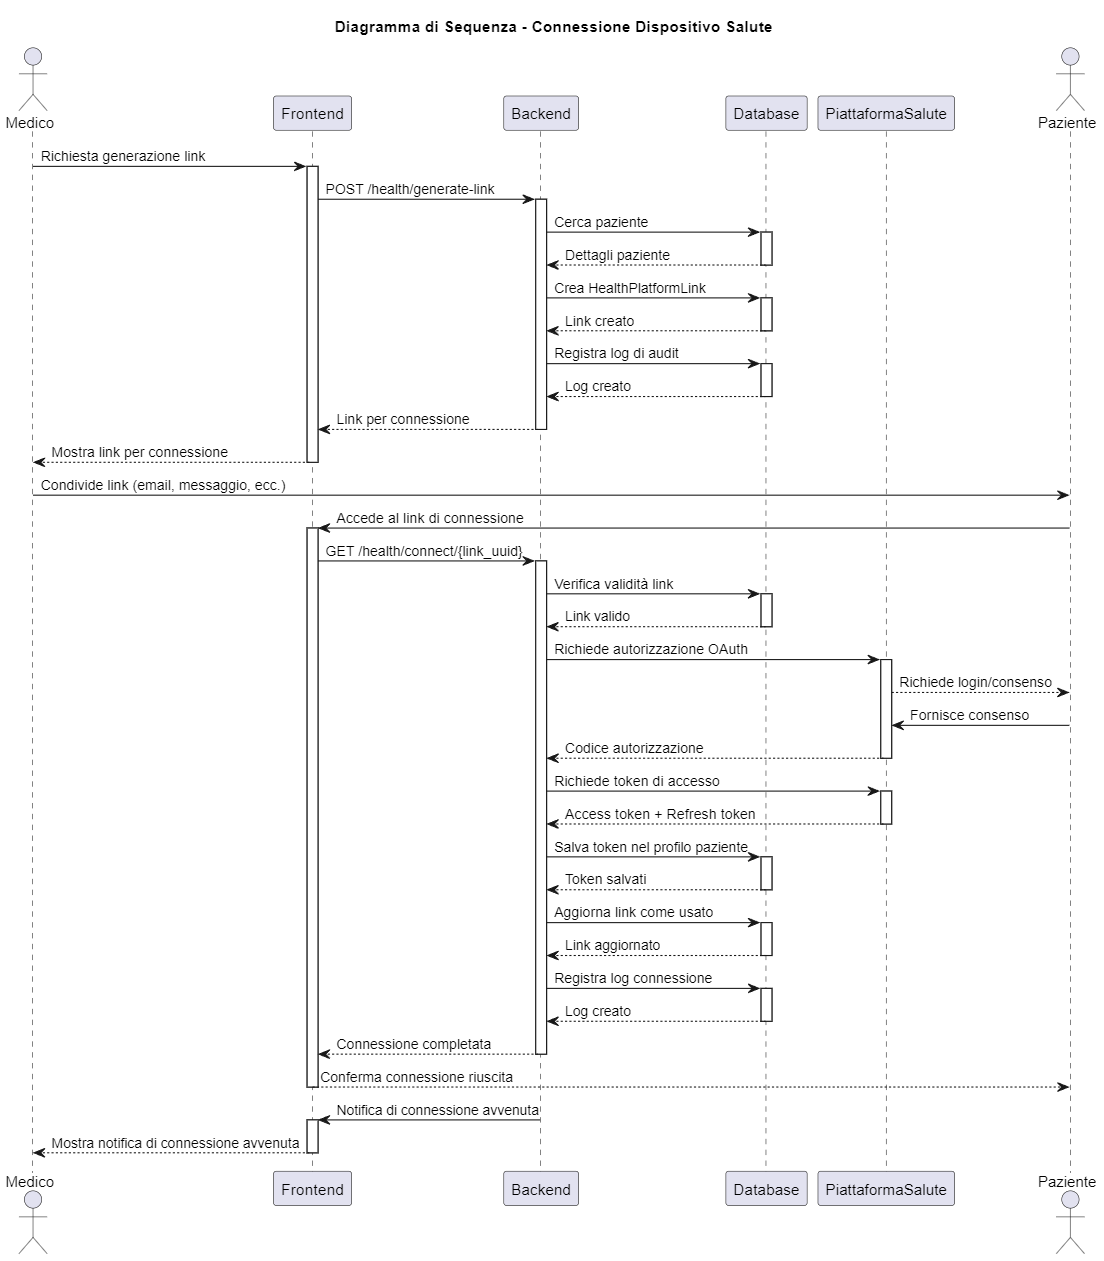
\includegraphics[width=0.85\textwidth]{images/uml/HealthDeviceConnection.png}
    \caption{Grafico UML di sequenza per la connessione al dispositivo}
    \label{fig:uml-seq-conn-graph}
\end{figure}
\begin{figure}[H]
    \centering
    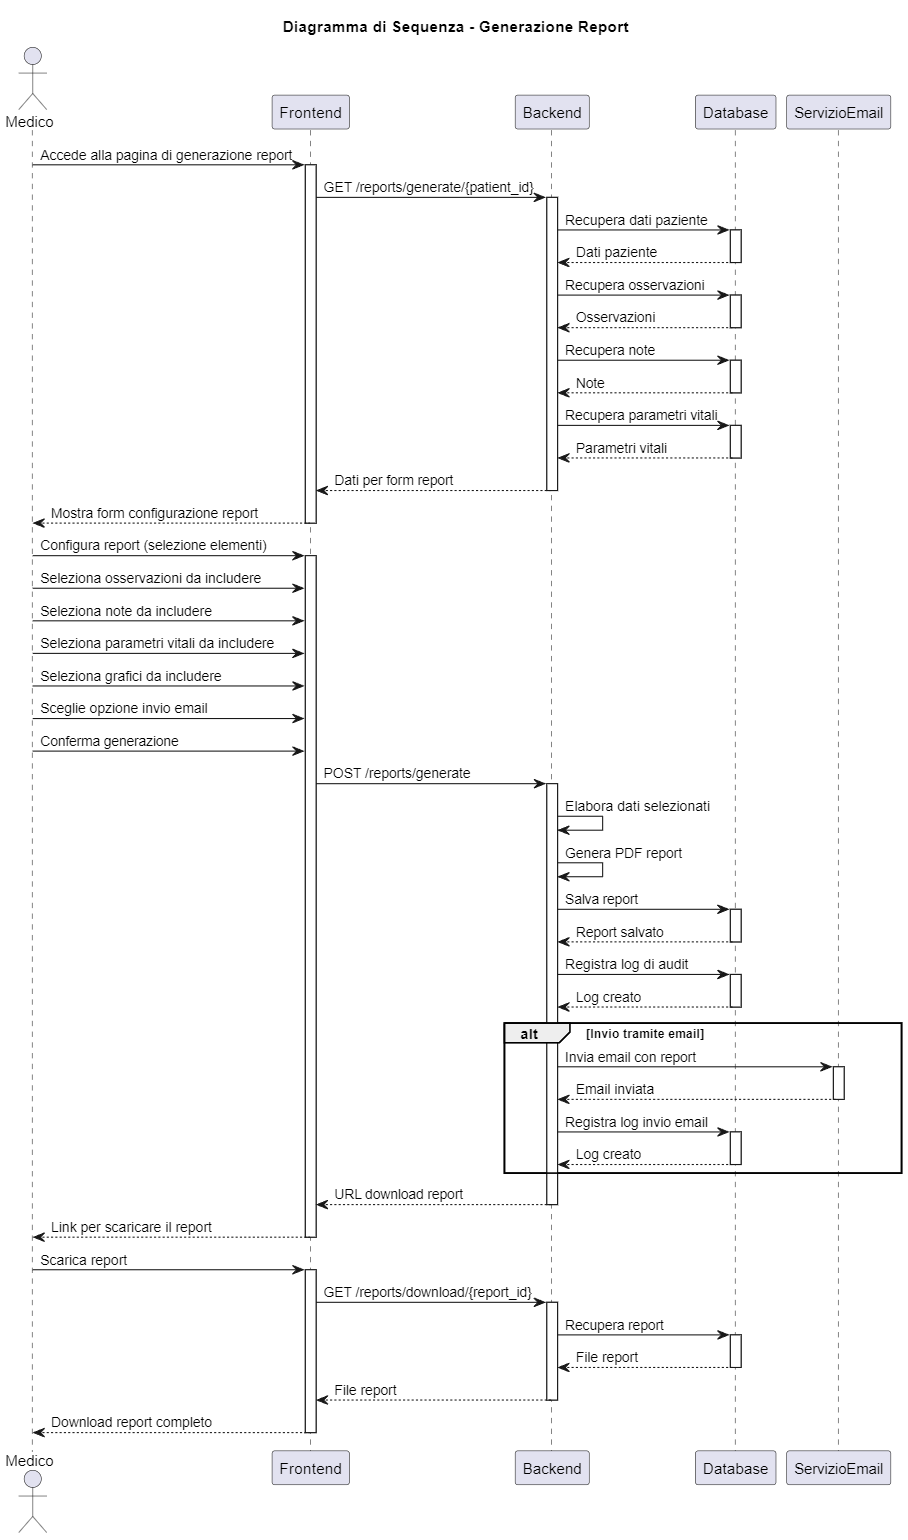
\includegraphics[width=0.85\textwidth]{images/uml/ReportGeneration.png}
    \caption{Grafico UML di sequenza per la generazione del report}
    \label{fig:uml-seq-report}
\end{figure}
\begin{lstlisting}[basicstyle=\small\ttfamily, breaklines=true, caption={connessione al dispositivo}]
@startuml "DiagrammaSequenza-ConnessioneDispositivo"

' Sequence diagram for connecting health devices
title Diagramma di Sequenza - Connessione Dispositivo Salute

actor "Medico" as Doctor
participant "Frontend" as Frontend
participant "Backend" as Backend
participant "Database" as DB
participant "PiattaformaSalute" as HealthPlatform
actor "Paziente" as Patient

' Generate connection link
Doctor -> Frontend: Richiesta generazione link
activate Frontend
Frontend -> Backend: POST /health/generate-link
activate Backend
Backend -> DB: Cerca paziente
activate DB
DB --> Backend: Dettagli paziente
deactivate DB
Backend -> DB: Crea HealthPlatformLink
activate DB
DB --> Backend: Link creato
deactivate DB
Backend -> DB: Registra log di audit
activate DB
DB --> Backend: Log creato
deactivate DB
Backend --> Frontend: Link per connessione
deactivate Backend
Frontend --> Doctor: Mostra link per connessione
deactivate Frontend

' Share link with patient
Doctor -> Patient: Condivide link (email, messaggio, ecc.)

' Patient uses the link
Patient -> Frontend: Accede al link di connessione
activate Frontend
Frontend -> Backend: GET /health/connect/{link_uuid}
activate Backend
Backend -> DB: Verifica validita' link
activate DB
DB --> Backend: Link valido
deactivate DB
Backend -> HealthPlatform: Richiede autorizzazione OAuth
activate HealthPlatform
HealthPlatform --> Patient: Richiede login/consenso
Patient -> HealthPlatform: Fornisce consenso
HealthPlatform --> Backend: Codice autorizzazione
deactivate HealthPlatform

' Exchange authorization code for tokens
Backend -> HealthPlatform: Richiede token di accesso
activate HealthPlatform
HealthPlatform --> Backend: Access token + Refresh token
deactivate HealthPlatform

' Save tokens to database
Backend -> DB: Salva token nel profilo paziente
activate DB
DB --> Backend: Token salvati
deactivate DB
Backend -> DB: Aggiorna link come usato
activate DB
DB --> Backend: Link aggiornato
deactivate DB
Backend -> DB: Registra log connessione
activate DB
DB --> Backend: Log creato
deactivate DB
Backend --> Frontend: Connessione completata
deactivate Backend
Frontend --> Patient: Conferma connessione riuscita
deactivate Frontend

' Notify doctor
Backend -> Frontend: Notifica di connessione avvenuta
activate Frontend
Frontend --> Doctor: Mostra notifica di connessione avvenuta
deactivate Frontend

@enduml

\end{lstlisting}
\begin{lstlisting}[basicstyle=\small\ttfamily, breaklines=true, caption={generazione del report}]
@startuml "DiagrammaSequenza-GenerazioneReport"

' Sequence diagram for report generation
title Diagramma di Sequenza - Generazione Report

actor "Medico" as Doctor
participant "Frontend" as Frontend
participant "Backend" as Backend
participant "Database" as DB
participant "ServizioEmail" as EmailService

' Start report generation
Doctor -> Frontend: Accede alla pagina di generazione report
activate Frontend
Frontend -> Backend: GET /reports/generate/{patient_id}
activate Backend
Backend -> DB: Recupera dati paziente
activate DB
DB --> Backend: Dati paziente
deactivate DB
Backend -> DB: Recupera osservazioni
activate DB
DB --> Backend: Osservazioni
deactivate DB
Backend -> DB: Recupera note
activate DB
DB --> Backend: Note
deactivate DB
Backend -> DB: Recupera parametri vitali
activate DB
DB --> Backend: Parametri vitali
deactivate DB
Backend --> Frontend: Dati per form report
deactivate Backend
Frontend --> Doctor: Mostra form configurazione report
deactivate Frontend

' Configure report
Doctor -> Frontend: Configura report (selezione elementi)
activate Frontend
Doctor -> Frontend: Seleziona osservazioni da includere
Doctor -> Frontend: Seleziona note da includere
Doctor -> Frontend: Seleziona parametri vitali da includere
Doctor -> Frontend: Seleziona grafici da includere
Doctor -> Frontend: Sceglie opzione invio email
Doctor -> Frontend: Conferma generazione
Frontend -> Backend: POST /reports/generate
activate Backend

' Generate report
Backend -> Backend: Elabora dati selezionati
Backend -> Backend: Genera PDF report
Backend -> DB: Salva report
activate DB
DB --> Backend: Report salvato
deactivate DB
Backend -> DB: Registra log di audit
activate DB
DB --> Backend: Log creato
deactivate DB

' Handle email option if selected
alt Invio tramite email
    Backend -> EmailService: Invia email con report
    activate EmailService
    EmailService --> Backend: Email inviata
    deactivate EmailService
    Backend -> DB: Registra log invio email
    activate DB
    DB --> Backend: Log creato
    deactivate DB
end

Backend --> Frontend: URL download report
deactivate Backend
Frontend --> Doctor: Link per scaricare il report
deactivate Frontend

' Download report
Doctor -> Frontend: Scarica report
activate Frontend
Frontend -> Backend: GET /reports/download/{report_id}
activate Backend
Backend -> DB: Recupera report
activate DB
DB --> Backend: File report
deactivate DB
Backend --> Frontend: File report
deactivate Backend
Frontend --> Doctor: Download report completo
deactivate Frontend

@enduml


\end{lstlisting}
\section{Diagrammi di stato}
\begin{figure}[H]
    \centering
    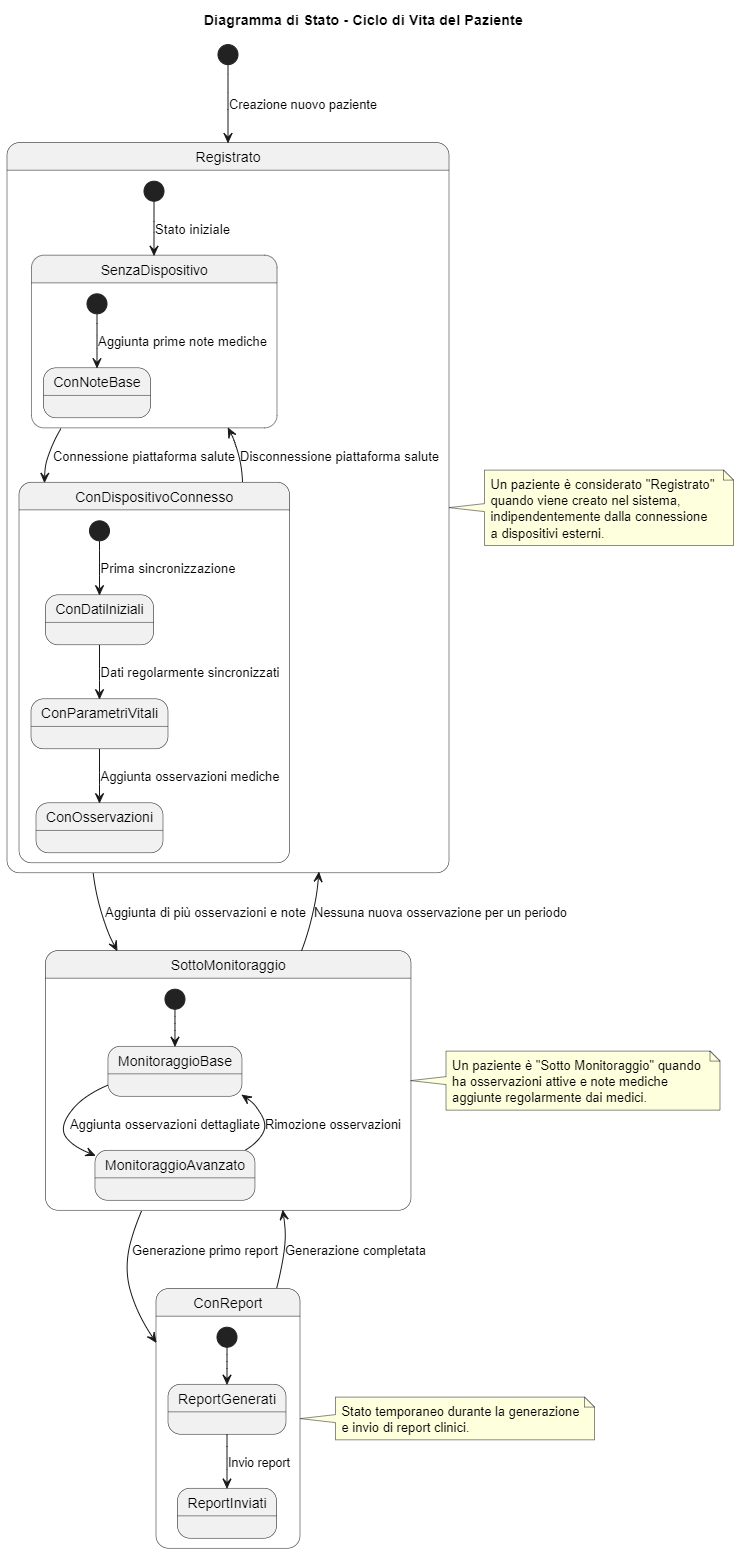
\includegraphics[width=0.85\textwidth]{images/uml/PatientLifecycle.png}
    \caption{Grafico UML di stato per il ciclo di vita del paziente}
    \label{fig:uml-state-graph}
\end{figure}

\begin{lstlisting}[basicstyle=\small\ttfamily, breaklines=true, caption={ciclo di vita del paziente}]
@startuml "DiagrammaStati-CicloVitaPaziente"

' State diagram for patient lifecycle
title Diagramma di Stato - Ciclo di Vita del Paziente

[*] --> Registrato : Creazione nuovo paziente

state Registrato {
  [*] --> SenzaDispositivo : Stato iniziale
  
  state SenzaDispositivo {
    [*] --> ConNoteBase : Aggiunta prime note mediche
  }
  
  state ConDispositivoConnesso {
    [*] --> ConDatiIniziali : Prima sincronizzazione
    ConDatiIniziali --> ConParametriVitali : Dati regolarmente sincronizzati
    ConParametriVitali --> ConOsservazioni : Aggiunta osservazioni mediche
  }
  
  SenzaDispositivo --> ConDispositivoConnesso : Connessione piattaforma salute
  ConDispositivoConnesso --> SenzaDispositivo : Disconnessione piattaforma salute
}

state "SottoMonitoraggio" as Monitorato {
  [*] --> MonitoraggioBase
  MonitoraggioBase --> MonitoraggioAvanzato : Aggiunta osservazioni dettagliate
  MonitoraggioAvanzato --> MonitoraggioBase : Rimozione osservazioni
}

Registrato --> Monitorato : Aggiunta di piu' osservazioni e note
Monitorato --> Registrato : Nessuna nuova osservazione per un periodo

state "ConReport" as Report {
  [*] --> ReportGenerati
  ReportGenerati --> ReportInviati : Invio report
}

Monitorato --> Report : Generazione primo report
Report --> Monitorato : Generazione completata

note right of Registrato
  Un paziente e' considerato "Registrato" 
  quando viene creato nel sistema,
  indipendentemente dalla connessione 
  a dispositivi esterni.
end note

note right of Monitorato
  Un paziente e' "Sotto Monitoraggio" quando 
  ha osservazioni attive e note mediche
  aggiunte regolarmente dai medici.
end note

note right of Report
  Stato temporaneo durante la generazione
  e invio di report clinici.
end note

@enduml

\end{lstlisting}
\section{Diagrammi delle attività}
\begin{figure}[H]
    \centering
    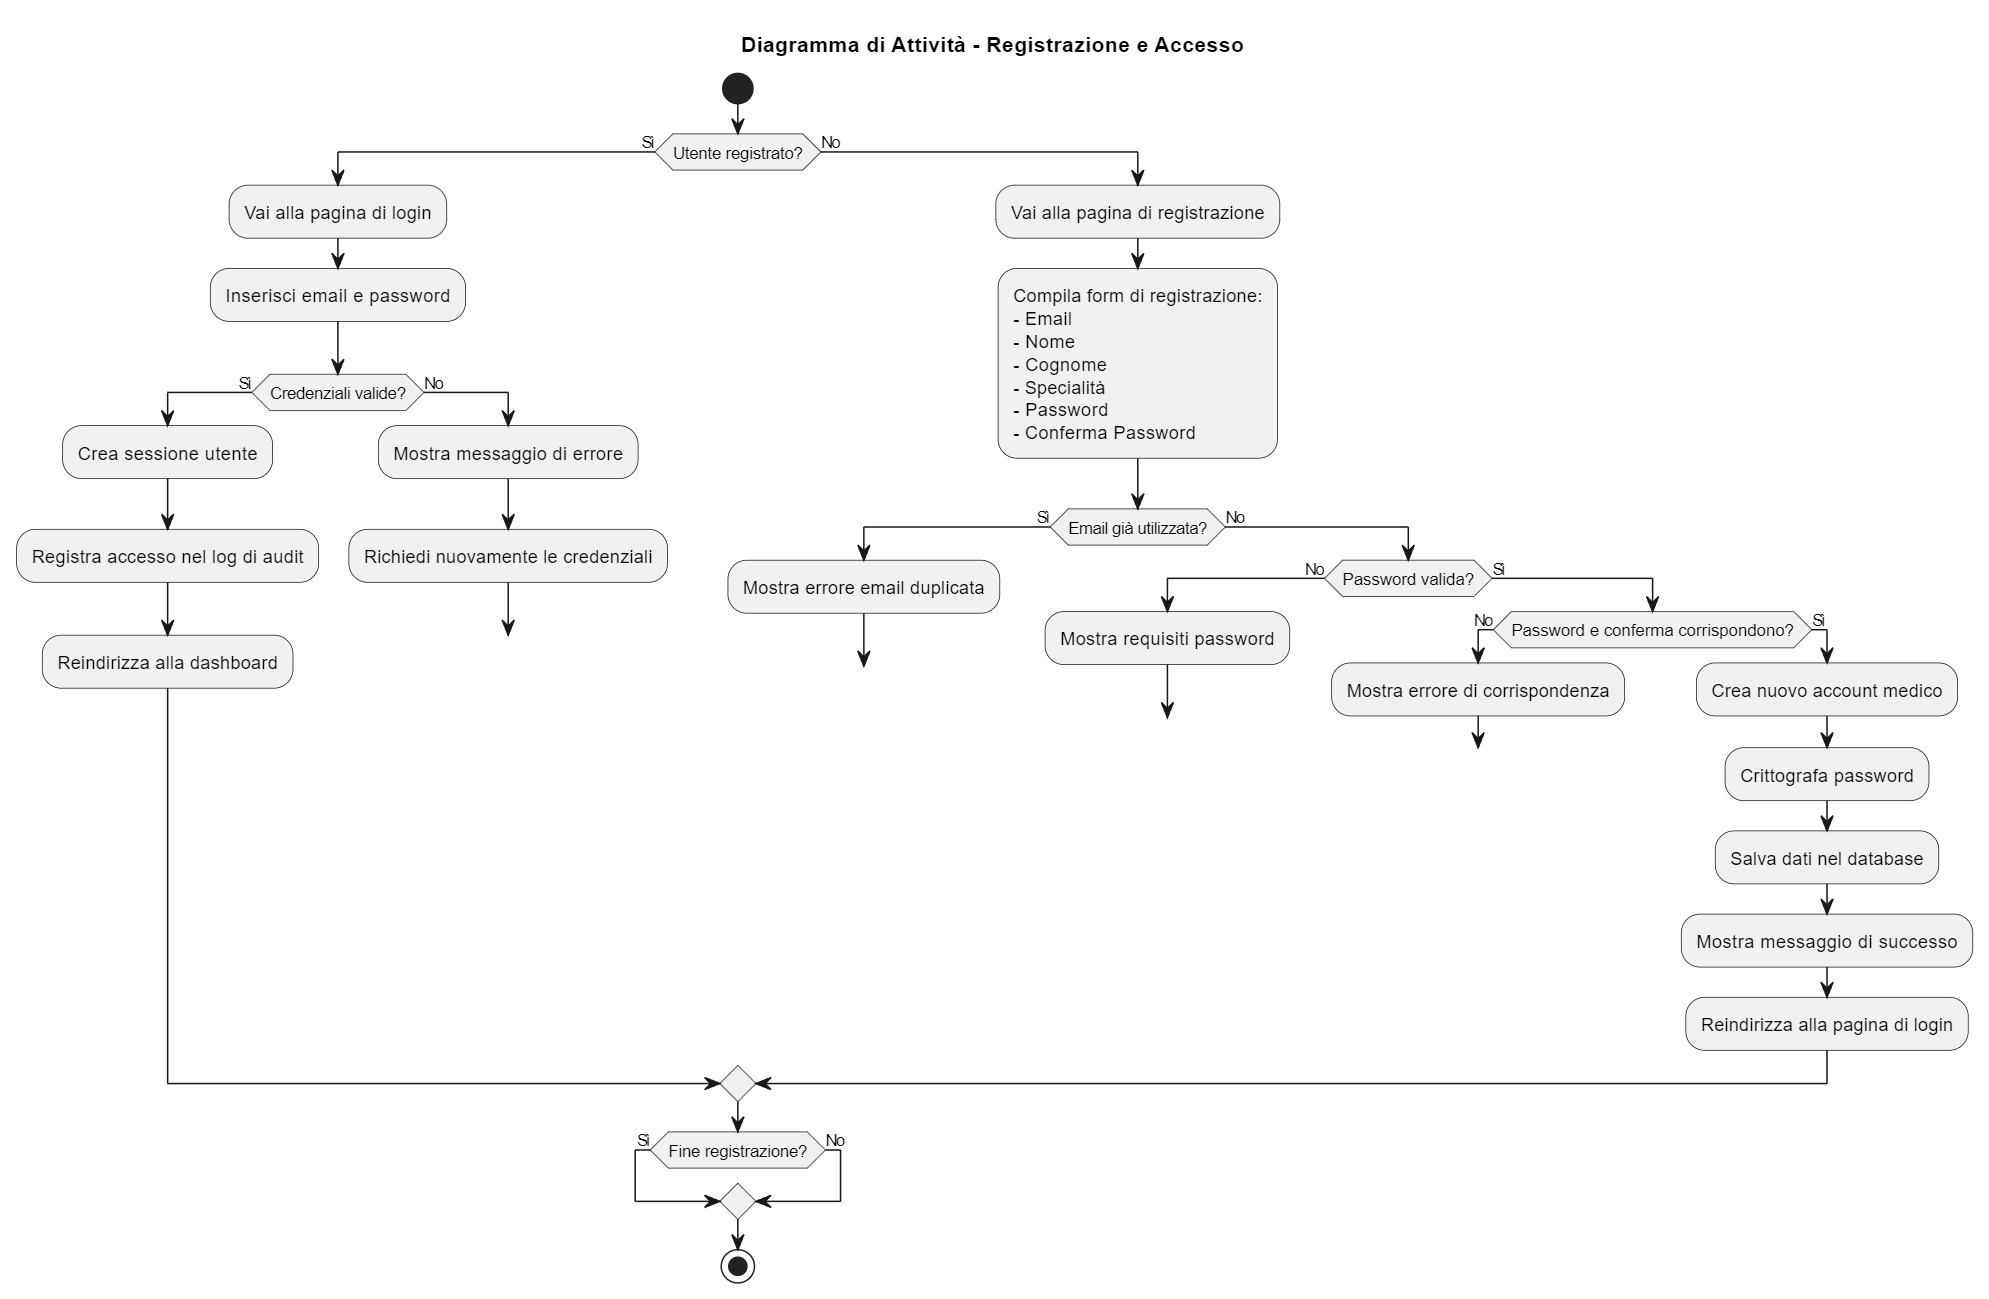
\includegraphics[width=0.85\textwidth]{images/uml/RegistrationLogin.png}
    \caption{Grafico UML di attività per la registrazione e il login}
    \label{fig:uml-act-graph}
\end{figure}
\begin{lstlisting}[basicstyle=\small\ttfamily, breaklines=true, caption={gestione del paziente}]
@startuml "DiagrammaAttivita-GestionePazienti"

' Activity diagram for patient data management
title Diagramma di Attivita' - Gestione Dati Pazienti

|Medico|
start
:Accede alla dashboard;
:Seleziona "Lista Pazienti";

|#AntiqueWhite|Sistema|
:Carica lista pazienti associati al medico;
:Visualizza pazienti con informazioni principali;

|Medico|
if (Desidera gestire un paziente esistente?) then (si')
  :Seleziona paziente dalla lista;
  
  |Sistema|
  :Carica dati completi del paziente;
  :Visualizza profilo dettagliato del paziente;
  
  |Medico|
  split
    :Visualizza dettagli paziente;
    
  split again
    :Seleziona "Modifica Paziente";
    
    |Sistema|
    :Mostra form di modifica paziente;
    
    |Medico|
    :Aggiorna dati paziente;
    :Invia form;
    
    |Sistema|
    :Valida dati;
    if (Dati validi?) then (si')
      :Salva modifiche;
      :Registra audit log;
      :Mostra conferma;
    else (no)
      :Mostra errori di validazione;
      :Richiede correzioni;
    endif
    
  split again
    :Seleziona "Parametri Vitali";
    
    |Sistema|
    if (Paziente connesso a piattaforma?) then (si')
      :Recupera parametri vitali da piattaforma;
      :Elabora e organizza dati;
      :Visualizza parametri vitali;
      
      |Medico|
      :Seleziona intervallo di visualizzazione;
      
      |Sistema|
      :Aggiorna visualizzazione per intervallo;
      
      |Medico|
      :Aggiunge osservazione sui parametri;
      
      |Sistema|
      :Salva nuova osservazione;
      :Registra audit log;
      
    else (no)
      :Mostra opzione di connessione;
      
      |Medico|
      if (Desidera connettere?) then (si')
        :Genera link per connessione;
        
        |Sistema|
        :Crea link unico;
        :Registra audit log;
        
        |Medico|
        :Condivide link con paziente;
        
        |#LightBlue|Paziente|
        :Utilizza link per connettere dispositivo;
        
        |Sistema|
        :Completa connessione;
        :Registra audit log;
        
      else (no)
        :Annulla processo;
      endif
    endif
    
  split again
    :Seleziona "Note";
    
    |Sistema|
    :Carica note esistenti;
    
    |Medico|
    :Visualizza note esistenti;
    if (Desidera aggiungere nota?) then (si')
      :Scrive nuova nota;
      :Invia nota;
      
      |Sistema|
      :Salva nuova nota;
      :Registra audit log;
      
    else (no)
      if (Desidera eliminare nota?) then (si')
        :Seleziona nota da eliminare;
        :Conferma eliminazione;
        
        |Sistema|
        :Elimina nota;
        :Registra audit log;
        
      else (no)
        :Nessuna azione;
      endif
    endif
    
  split again
    :Seleziona "Genera Report";
    
    |Sistema|
    :Mostra opzioni di configurazione report;
    
    |Medico|
    :Seleziona elementi da includere;
    :Seleziona formato e opzioni di invio;
    :Conferma generazione report;
    
    |Sistema|
    :Genera report PDF;
    if (Invio email selezionato?) then (si')
      :Invia report via email;
    else (no)
      :Prepara download;
    endif
    :Registra audit log;
    
  end split
  
else (no)
  if (Desidera creare nuovo paziente?) then (si')
    :Seleziona "Nuovo Paziente";
    
    |Sistema|
    :Mostra form nuovo paziente;
    
    |Medico|
    :Compila dati paziente;
    :Invia form;
    
    |Sistema|
    :Valida dati;
    if (Dati validi?) then (si')
      :Crea nuovo paziente;
      :Associa paziente al medico;
      :Registra audit log;
      :Mostra conferma;
    else (no)
      :Mostra errori di validazione;
      :Richiede correzioni;
    endif
    
  else (no)
    if (Desidera importare paziente?) then (si')
      :Seleziona "Importa Paziente";
      
      |Sistema|
      :Mostra form di importazione;
      
      |Medico|
      :Inserisce UUID paziente;
      :Invia form;
      
      |Sistema|
      :Verifica esistenza paziente;
      if (Paziente esiste?) then (si')
        :Associa paziente al medico;
        :Registra audit log;
        :Mostra conferma;
      else (no)
        :Mostra errore;
      endif
      
    else (no)
      :Torna alla dashboard;
    endif
  endif
endif

|Medico|
stop

@enduml

\end{lstlisting}

\begin{lstlisting}[basicstyle=\small\ttfamily, breaklines=true, caption={registrazione e accesso}]
@startuml "DiagrammaAttivita-RegistrazioneAccesso"

' Activity diagram for registration and login
title Diagramma di Attivita' - Registrazione e Accesso

start

' Initial decision - register or login
if (Utente registrato?) then (Si')
  :Vai alla pagina di login;
  :Inserisci email e password;
  
  if (Credenziali valide?) then (Si')
    :Crea sessione utente;
    :Registra accesso nel log di audit;
    :Reindirizza alla dashboard;
  else (No)
    :Mostra messaggio di errore;
    :Richiedi nuovamente le credenziali;
    goto EndLogin;
  endif
  
else (No)
  :Vai alla pagina di registrazione;
  :Compila form di registrazione:
  - Email
  - Nome
  - Cognome
  - Specialita'
  - Password
  - Conferma Password;
  
  if (Email gia' utilizzata?) then (Si')
    :Mostra errore email duplicata;
    goto EndRegistration;
  else (No)
    if (Password valida?) then (No)
      :Mostra requisiti password;
      goto EndRegistration;
    else (Si')
      if (Password e conferma corrispondono?) then (No)
        :Mostra errore di corrispondenza;
        goto EndRegistration;
      else (Si')
        :Crea nuovo account medico;
        :Crittografa password;
        :Salva dati nel database;
        :Mostra messaggio di successo;
        :Reindirizza alla pagina di login;
      endif
    endif
  endif
  
endif

' End markers for visual clarity
if (Fine registrazione?) then (Si')
  label EndRegistration
else (No)
  label EndLogin
endif

stop

@enduml

\end{lstlisting}
\section{Diagrammi di deployment}
\begin{figure}[H]
    \centering
    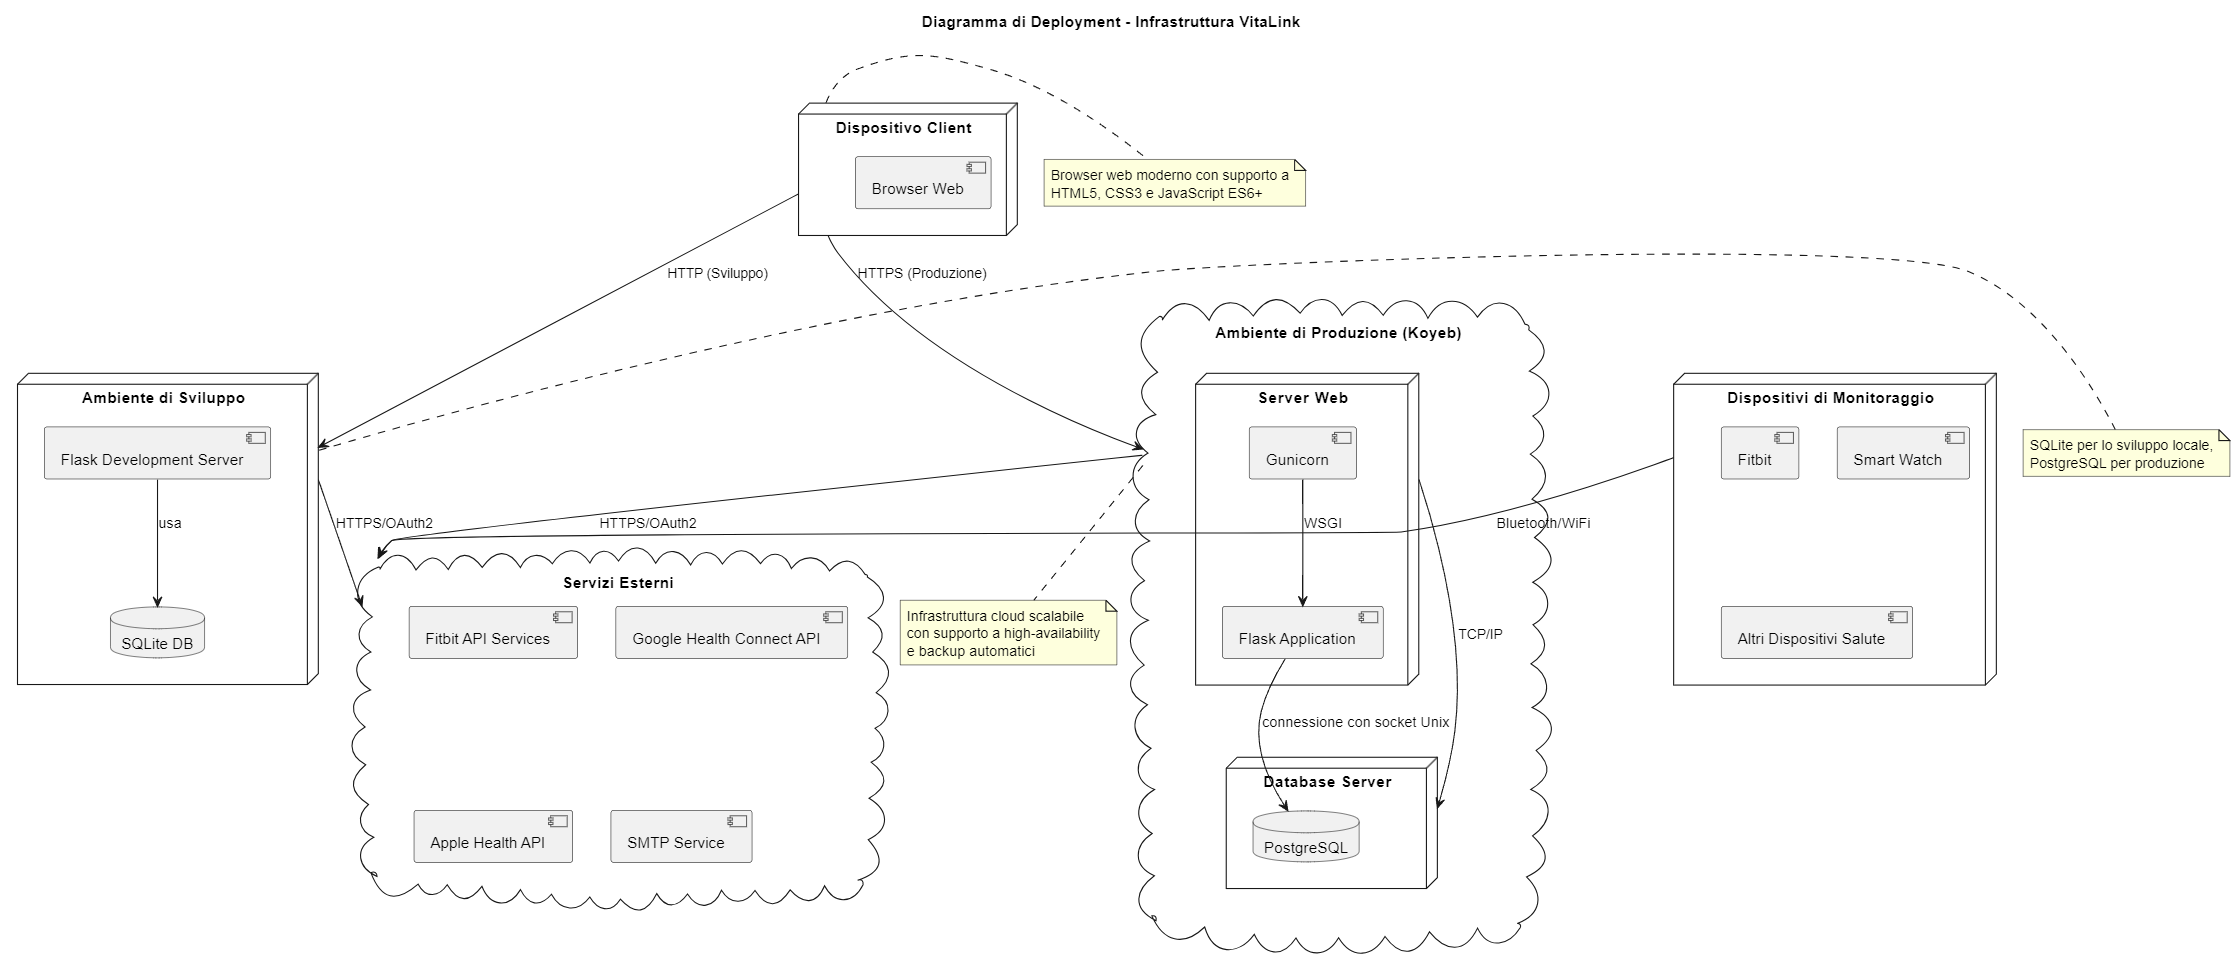
\includegraphics[width=0.85\textwidth]{images/uml/InfrastructureDeployment.png}
    \caption{Grafico UML di deployment}
    \label{fig:uml-depl-graph}
\end{figure}
\begin{lstlisting}[basicstyle=\small\ttfamily, breaklines=true]
@startuml "DiagrammaDeployment-InfrastruttraVitaLink"

' Deployment diagram for VitaLink infrastructure
title Diagramma di Deployment - Infrastruttura VitaLink

' Client devices
node "Dispositivo Client" as ClientDevice {
  component [Browser Web] as WebBrowser
}

' Development environment
node "Ambiente di Sviluppo" as DevEnv {
  component [Flask Development Server] as FlaskDev
  database "SQLite DB" as SQLiteDB
  
  FlaskDev --> SQLiteDB : usa
}

' Production Cloud environment
cloud "Ambiente di Produzione (Koyeb)" as ProdEnv {
  node "Server Web" as WebServer {
    component [Gunicorn] as Gunicorn
    component [Flask Application] as FlaskApp
    
    Gunicorn --> FlaskApp : WSGI
  }
  
  node "Database Server" as DBServer {
    database "PostgreSQL" as PostgreSQL
  }
  
  WebServer --> DBServer : TCP/IP
  FlaskApp --> PostgreSQL : connessione con socket Unix
}

' Third-party services
cloud "Servizi Esterni" as ExternalServices {
  component [Fitbit API Services] as FitbitAPI
  component [Google Health Connect API] as GoogleHealth
  component [Apple Health API] as AppleHealth
  component [SMTP Service] as SMTPService
}

' Connections
ClientDevice --> DevEnv : HTTP (Sviluppo)
ClientDevice --> ProdEnv : HTTPS (Produzione)
ProdEnv --> ExternalServices : HTTPS/OAuth2
DevEnv --> ExternalServices : HTTPS/OAuth2

' Equipment needed by devices
node "Dispositivi di Monitoraggio" as MonitoringDevices {
  component [Fitbit] as FitbitDevice
  component [Smart Watch] as SmartWatch
  component [Altri Dispositivi Salute] as OtherDevices
}

MonitoringDevices --> ExternalServices : Bluetooth/WiFi

' Deployment notes
note right of ClientDevice
  Browser web moderno con supporto a
  HTML5, CSS3 e JavaScript ES6+
end note

note bottom of ProdEnv
  Infrastruttura cloud scalabile
  con supporto a high-availability
  e backup automatici
end note

note right of DevEnv
  SQLite per lo sviluppo locale,
  PostgreSQL per produzione
end note

@enduml

\end{lstlisting}
\section{Diagrammi ER}
\begin{figure}[H]
    \centering
    \includegraphics[width=0.85\textwidth]{images/uml/DataModel.png}
    \caption{Grafico UML ER per il modello dati}
    \label{fig:uml-ER-graph}
\end{figure}
\begin{lstlisting}[basicstyle=\small\ttfamily, breaklines=true]
@startuml "DiagrammaER-ModelloDati"

' Entity Relationship diagram for VitaLink
title Diagramma ER - Modello Dati VitaLink

' Styling
!define TABLE_BORDER_COLOR #073B4C
!define PRIMARY_KEY_COLOR #06D6A0
!define FOREIGN_KEY_COLOR #EF476F
!define ATTRIBUTE_COLOR #118AB2
!define ENUM_COLOR #FFD166
skinparam linetype ortho
skinparam roundcorner 15

' Enum Entities
entity "VitalSignType" as VitalSignType << Enum >> {
  + HEART_RATE
  + OXYGEN_SATURATION
  + BREATHING_RATE
  + WEIGHT
  + TEMPERATURE_CORE
  + TEMPERATURE_SKIN
  + STEPS
  + CALORIES
  + DISTANCE
  + ACTIVE_MINUTES
  + SLEEP_DURATION
  + ...altri tipi di parametri vitali
}

entity "HealthPlatform" as HealthPlatform << Enum >> {
  + FITBIT
  + GOOGLE_HEALTH_CONNECT
  + APPLE_HEALTH
}

entity "ActionType" as ActionType << Enum >> {
  + CREATE
  + UPDATE
  + DELETE
  + VIEW
  + EXPORT
  + GENERATE_LINK
  + CONNECT
  + DISCONNECT
  + SYNC
  + IMPORT
}

entity "EntityType" as EntityType << Enum >> {
  + PATIENT
  + VITAL_SIGN
  + NOTE
  + REPORT
  + HEALTH_PLATFORM
  + HEALTH_LINK
  + OBSERVATION
}

' Main Entities
entity "Doctor" as Doctor {
  * id : Integer <<PK>>
  --
  * email : String <<unique>>
  * password_hash : String
  * first_name : String
  * last_name : String
  specialty : String
  * created_at : DateTime
  * updated_at : DateTime
}

entity "Patient" as Patient {
  * id : Integer <<PK>>
  --
  * uuid : String <<unique>>
  * first_name : String
  * last_name : String
  * date_of_birth : Date
  gender : String
  * contact_number : String
  email : String
  address : Text
  * created_at : DateTime
  * updated_at : DateTime
  connected_platform : HealthPlatform <<FK>>
  platform_access_token : String
  platform_refresh_token : String
  platform_token_expires_at : DateTime
}

entity "DoctorPatient" as DoctorPatient {
  * doctor_id : Integer <<PK, FK>>
  * patient_id : Integer <<PK, FK>>
  * assigned_date : DateTime
}

entity "Note" as Note {
  * id : Integer <<PK>>
  --
  * patient_id : Integer <<FK>>
  * doctor_id : Integer <<FK>>
  * content : Text
  * created_at : DateTime
  * updated_at : DateTime
}

entity "VitalObservation" as VitalObservation {
  * id : Integer <<PK>>
  --
  * patient_id : Integer <<FK>>
  * doctor_id : Integer <<FK>>
  * vital_type : VitalSignType <<FK>>
  * content : Text
  * start_date : DateTime
  * end_date : DateTime
  * created_at : DateTime
  * updated_at : DateTime
}

entity "AuditLog" as AuditLog {
  * id : Integer <<PK>>
  --
  * doctor_id : Integer <<FK>>
  * timestamp : DateTime
  * action_type : ActionType <<FK>>
  * entity_type : EntityType <<FK>>
  * entity_id : Integer
  details : Text
  patient_id : Integer <<FK>>
  ip_address : String
}

entity "HealthPlatformLink" as HealthPlatformLink {
  * id : Integer <<PK>>
  --
  * uuid : String <<unique>>
  * patient_id : Integer <<FK>>
  * doctor_id : Integer <<FK>>
  * created_at : DateTime
  * expires_at : DateTime
  * used : Boolean
  * platform : HealthPlatform <<FK>>
}

' Define the relationships
Doctor ||--o{ DoctorPatient
Patient ||--o{ DoctorPatient

Doctor ||--o{ Note
Patient ||--o{ Note

Doctor ||--o{ VitalObservation
Patient ||--o{ VitalObservation
VitalSignType ||--o{ VitalObservation

Doctor ||--o{ AuditLog
Patient |o--o{ AuditLog
ActionType ||--o{ AuditLog
EntityType ||--o{ AuditLog

Doctor ||--o{ HealthPlatformLink
Patient ||--o{ HealthPlatformLink
HealthPlatform ||--o{ HealthPlatformLink

HealthPlatform |o--o{ Patient

@enduml

\end{lstlisting}
\section{Diagrammi di comunicazione}
\begin{figure}[H]
    \centering
    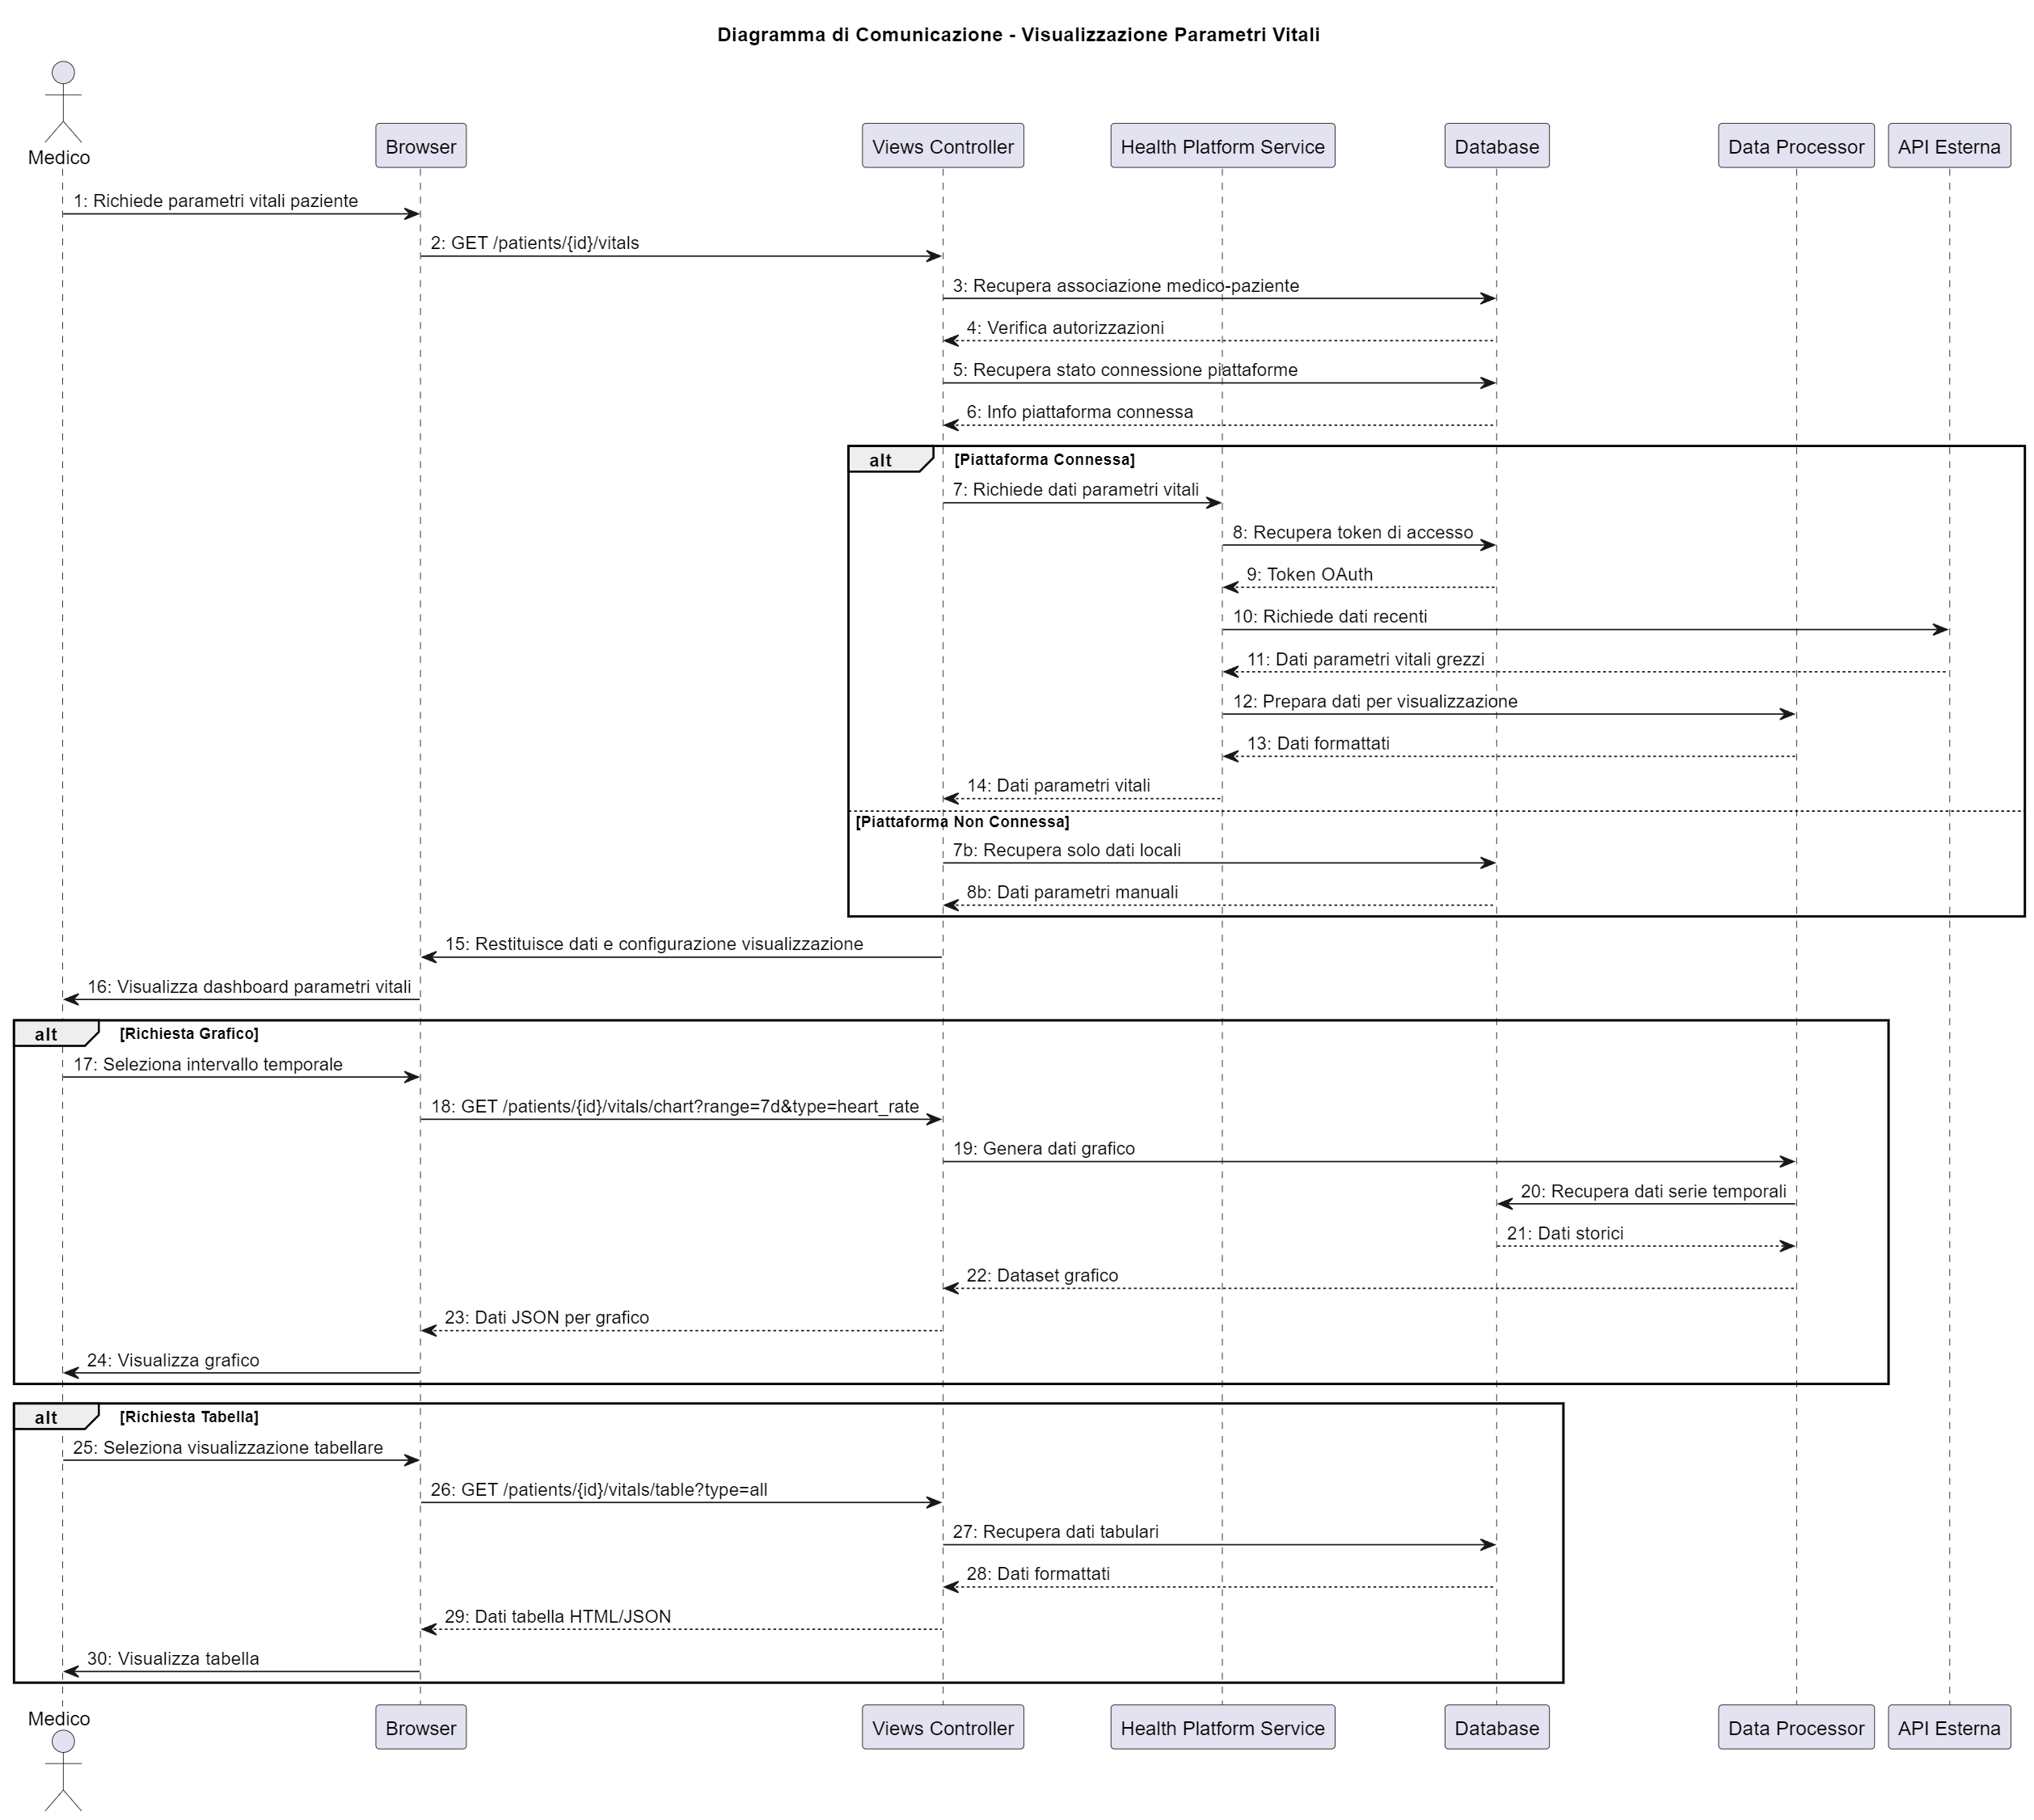
\includegraphics[width=0.85\textwidth]{images/uml/VitalSignsVisualization.png}
    \caption{Grafico UML di comunicazione per la visualizzazione dei parametri vitali}
    \label{fig:uml-com-vit-graph}
\end{figure}
\begin{lstlisting}[basicstyle=\small\ttfamily, breaklines=true, caption={visualizzazione dei parametri vitali}]
@startuml "DiagrammaComunicazione-ParametriVitali"

' Communication diagram for vital signs visualization
title Diagramma di Comunicazione - Visualizzazione Parametri Vitali

' Define the actors and components
actor "Medico" as Doctor
participant "Browser" as Browser
participant "Views Controller" as Views
participant "Health Platform Service" as HPS
participant "Database" as DB
participant "Data Processor" as Processor

' Communication paths for vital sign visualization
Doctor -> Browser : 1: Richiede parametri vitali paziente
Browser -> Views : 2: GET /patients/{id}/vitals
Views -> DB : 3: Recupera associazione medico-paziente
DB --> Views : 4: Verifica autorizzazioni

Views -> DB : 5: Recupera stato connessione piattaforme
DB --> Views : 6: Info piattaforma connessa

alt Piattaforma Connessa
  Views -> HPS : 7: Richiede dati parametri vitali
  HPS -> DB : 8: Recupera token di accesso
  DB --> HPS : 9: Token OAuth
  
  HPS -> "API Esterna" : 10: Richiede dati recenti
  "API Esterna" --> HPS : 11: Dati parametri vitali grezzi
  
  HPS -> Processor : 12: Prepara dati per visualizzazione
  Processor --> HPS : 13: Dati formattati
  
  HPS --> Views : 14: Dati parametri vitali
else Piattaforma Non Connessa
  Views -> DB : 7b: Recupera solo dati locali
  DB --> Views : 8b: Dati parametri manuali
end

Views -> Browser : 15: Restituisce dati e configurazione visualizzazione
Browser -> Doctor : 16: Visualizza dashboard parametri vitali

alt Richiesta Grafico
  Doctor -> Browser : 17: Seleziona intervallo temporale
  Browser -> Views : 18: GET /patients/{id}/vitals/chart?range=7d&type=heart_rate
  Views -> Processor : 19: Genera dati grafico
  Processor -> DB : 20: Recupera dati serie temporali
  DB --> Processor : 21: Dati storici
  Processor --> Views : 22: Dataset grafico
  Views --> Browser : 23: Dati JSON per grafico
  Browser -> Doctor : 24: Visualizza grafico
end

alt Richiesta Tabella
  Doctor -> Browser : 25: Seleziona visualizzazione tabellare
  Browser -> Views : 26: GET /patients/{id}/vitals/table?type=all
  Views -> DB : 27: Recupera dati tabulari
  DB --> Views : 28: Dati formattati
  Views --> Browser : 29: Dati tabella HTML/JSON
  Browser -> Doctor : 30: Visualizza tabella
end

@enduml

\end{lstlisting}
\section{Diagrammi delle componenti}
\begin{figure}[H]
    \centering
    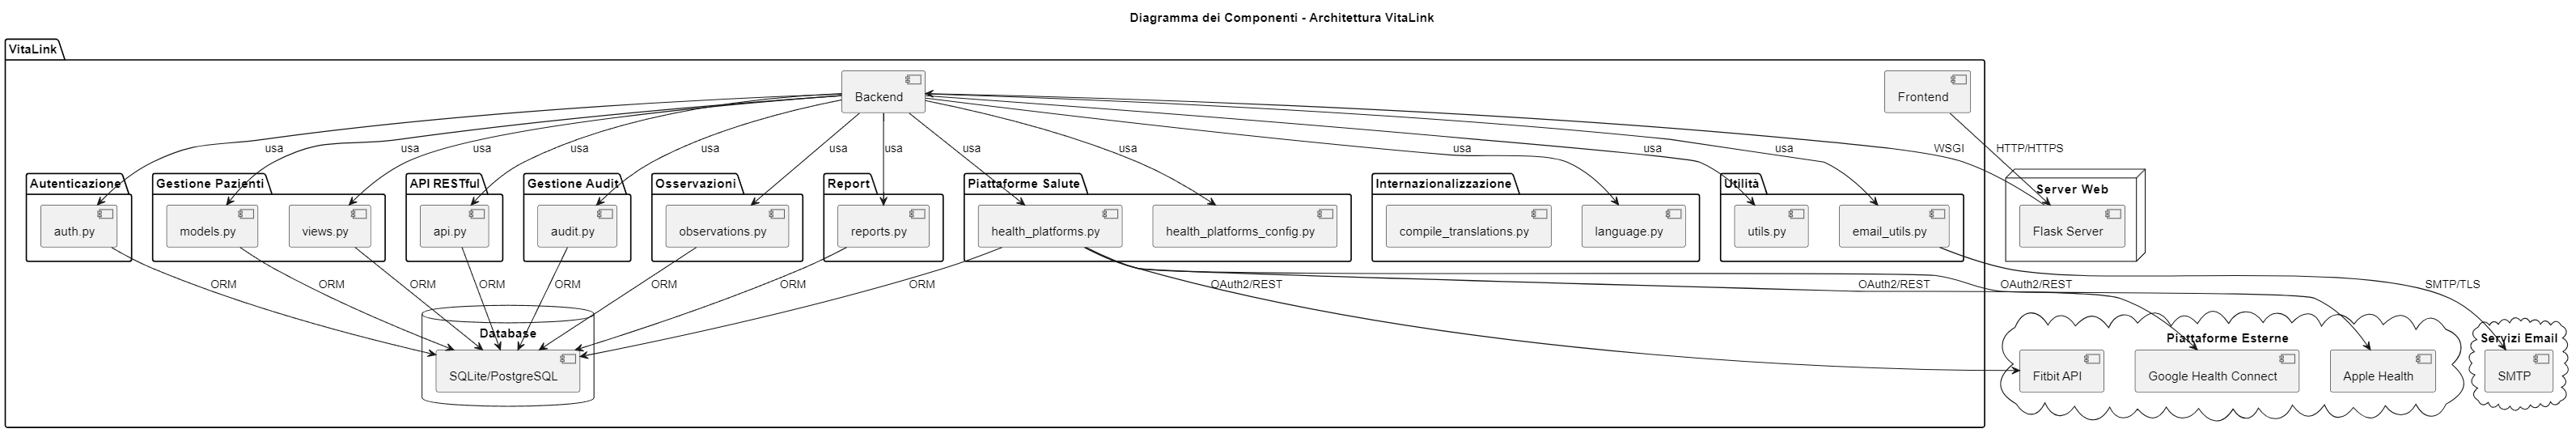
\includegraphics[width=0.85\textwidth]{images/uml/SystemArchitecture.png}
    \caption{Grafico UML delle componenti per l'architettura del sistema}
    \label{fig:uml-comp-graph}
\end{figure}
\begin{lstlisting}[basicstyle=\small\ttfamily, breaklines=true]
@startuml "DiagrammaComponenti-ArchitetturaVitaLink"

' Component diagram for VitaLink architecture
title Diagramma dei Componenti - Architettura VitaLink

' Main application package
package "VitaLink" {
  ' Core components
  [Frontend] as FE
  [Backend] as BE
  
  ' Application modules
  package "Autenticazione" {
    [auth.py] as Auth
  }
  
  package "Gestione Pazienti" {
    [views.py] as Views
    [models.py] as Models
  }
  
  package "API RESTful" {
    [api.py] as API
  }
  
  package "Gestione Audit" {
    [audit.py] as Audit
  }
  
  package "Piattaforme Salute" {
    [health_platforms.py] as HealthPlatforms
    [health_platforms_config.py] as HealthConfig
  }
  
  package "Osservazioni" {
    [observations.py] as Observations
  }
  
  package "Report" {
    [reports.py] as Reports
  }
  
  package "Internazionalizzazione" {
    [language.py] as Language
    [compile_translations.py] as Translations
  }
  
  package "Utilita'" {
    [utils.py] as Utils
    [email_utils.py] as Email
  }
  
  ' Database
  database "Database" {
    [SQLite/PostgreSQL] as DB
  }
}

' External systems
cloud "Piattaforme Esterne" {
  [Fitbit API] as FitbitAPI
  [Google Health Connect] as GoogleHealth
  [Apple Health] as AppleHealth
}

' Web Server
node "Server Web" {
  [Flask Server] as FlaskServer
}

' Email Services
cloud "Servizi Email" {
  [SMTP] as SMTP
}

' Relationships
FE --> FlaskServer : HTTP/HTTPS
FlaskServer --> BE : WSGI

' Backend Components Relationships
BE --> Auth : usa
BE --> Views : usa
BE --> Models : usa
BE --> API : usa
BE --> Audit : usa
BE --> HealthPlatforms : usa
BE --> HealthConfig : usa
BE --> Observations : usa
BE --> Reports : usa
BE --> Language : usa
BE --> Utils : usa
BE --> Email : usa

' External Communication
HealthPlatforms --> FitbitAPI : OAuth2/REST
HealthPlatforms --> GoogleHealth : OAuth2/REST
HealthPlatforms --> AppleHealth : OAuth2/REST
Email --> SMTP : SMTP/TLS

' Database Access
Models --> DB : ORM
Auth --> DB : ORM
Views --> DB : ORM
API --> DB : ORM
Audit --> DB : ORM
HealthPlatforms --> DB : ORM
Observations --> DB : ORM
Reports --> DB : ORM

@enduml

\end{lstlisting}
\section{Diagrammi degli oggetti}
\begin{lstlisting}[basicstyle=\small\ttfamily, breaklines=true]
@startuml "DiagrammaOggetti-EsempioIstanze"

' Object diagram showing instance examples for the VitaLink application
title Diagramma degli Oggetti - Esempio di Istanze

' Doctor objects
object "dott_rossi:Doctor" as DoctorRossi {
  id = 1
  email = "mario.rossi@medico.it"
  password_hash = "hashed_password_123"
  first_name = "Mario"
  last_name = "Rossi"
  specialty = "Cardiologia"
  created_at = "2025-01-10T09:30:00"
  updated_at = "2025-01-10T09:30:00"
}

object "dott_bianchi:Doctor" as DoctorBianchi {
  id = 2
  email = "laura.bianchi@medico.it"
  password_hash = "hashed_password_456"
  first_name = "Laura"
  last_name = "Bianchi"
  specialty = "Pneumologia"
  created_at = "2025-01-15T14:20:00"
  updated_at = "2025-01-15T14:20:00"
}

' Patient objects
object "paziente_verdi:Patient" as PatientVerdi {
  id = 1
  uuid = "f47ac10b-58cc-4372-a567-0e02b2c3d479"
  first_name = "Giuseppe"
  last_name = "Verdi"
  date_of_birth = "1970-05-15"
  gender = "Maschio"
  contact_number = "+39 333 1234567"
  email = "giuseppe.verdi@email.it"
  address = "Via Roma 123, Milano"
  created_at = "2025-02-01T10:15:00"
  updated_at = "2025-02-01T10:15:00"
  connected_platform = "FITBIT"
  platform_access_token = "ya29.a0AWY_..."
  platform_token_expires_at = "2025-05-10T10:15:00"
}

object "paziente_neri:Patient" as PatientNeri {
  id = 2
  uuid = "a97ac10b-12cc-8372-b567-0e02b2c3d123"
  first_name = "Anna"
  last_name = "Neri"
  date_of_birth = "1985-08-22"
  gender = "Femmina"
  contact_number = "+39 333 7654321"
  email = "anna.neri@email.it"
  created_at = "2025-02-10T11:30:00"
  updated_at = "2025-02-10T11:30:00"
  connected_platform = null
}

' Association objects
object "assoc_rossi_verdi:DoctorPatient" as AssocRossiVerdi {
  doctor_id = 1
  patient_id = 1
  assigned_date = "2025-02-01T10:15:00"
}

object "assoc_bianchi_verdi:DoctorPatient" as AssocBianchiVerdi {
  doctor_id = 2
  patient_id = 1
  assigned_date = "2025-03-15T09:20:00"
}

object "assoc_rossi_neri:DoctorPatient" as AssocRossiNeri {
  doctor_id = 1
  patient_id = 2
  assigned_date = "2025-02-10T11:30:00"
}

' Note objects
object "nota_1:Note" as Note1 {
  id = 1
  patient_id = 1
  doctor_id = 1
  content = "Paziente presenta ipertensione lieve. Consigliato monitoraggio frequente della pressione."
  created_at = "2025-02-01T10:30:00"
  updated_at = "2025-02-01T10:30:00"
}

object "nota_2:Note" as Note2 {
  id = 2
  patient_id = 1
  doctor_id = 2
  content = "Valori di saturazione dell'ossigeno nella norma. Nessun problema respiratorio riscontrato."
  created_at = "2025-03-15T09:45:00"
  updated_at = "2025-03-15T09:45:00"
}

' Vital observation objects
object "osservazione_1:VitalObservation" as Observation1 {
  id = 1
  patient_id = 1
  doctor_id = 1
  vital_type = "HEART_RATE"
  content = "Frequenza cardiaca elevata durante l'attivita' fisica. Valori nella norma a riposo."
  start_date = "2025-04-01T00:00:00"
  end_date = "2025-04-07T23:59:59"
  created_at = "2025-04-08T09:15:00"
  updated_at = "2025-04-08T09:15:00"
}

object "osservazione_2:VitalObservation" as Observation2 {
  id = 2
  patient_id = 1
  doctor_id = 1
  vital_type = "STEPS"
  content = "Livello di attivita' fisica buono. Media di 8000 passi al giorno nell'ultima settimana."
  start_date = "2025-04-01T00:00:00"
  end_date = "2025-04-07T23:59:59"
  created_at = "2025-04-08T09:20:00"
  updated_at = "2025-04-08T09:20:00"
}

' Health platform link object
object "link_piattaforma_1:HealthPlatformLink" as PlatformLink1 {
  id = 1
  uuid = "e47ac10b-58cc-4372-a567-0e02b2c3d480"
  patient_id = 1
  doctor_id = 1
  created_at = "2025-03-01T14:30:00"
  expires_at = "2025-03-02T14:30:00"
  used = true
  platform = "FITBIT"
}

' Audit log objects
object "audit_1:AuditLog" as Audit1 {
  id = 1
  doctor_id = 1
  timestamp = "2025-02-01T10:15:00"
  action_type = "CREATE"
  entity_type = "PATIENT"
  entity_id = 1
  details = "{'notes': 'Creazione nuovo paziente'}"
  patient_id = 1
  ip_address = "192.168.1.100"
}

object "audit_2:AuditLog" as Audit2 {
  id = 2
  doctor_id = 1
  timestamp = "2025-03-01T14:30:00"
  action_type = "GENERATE_LINK"
  entity_type = "HEALTH_LINK"
  entity_id = 1
  details = "{'platform': 'FITBIT', 'expires_at': '2025-03-02T14:30:00'}"
  patient_id = 1
  ip_address = "192.168.1.100"
}

object "audit_3:AuditLog" as Audit3 {
  id = 3
  doctor_id = 1
  timestamp = "2025-03-01T16:45:00"
  action_type = "CONNECT"
  entity_type = "HEALTH_PLATFORM"
  entity_id = 1
  details = "{'platform': 'FITBIT', 'status': 'success'}"
  patient_id = 1
  ip_address = "203.0.113.42"
}

' Relationships
DoctorRossi -- AssocRossiVerdi
PatientVerdi -- AssocRossiVerdi

DoctorBianchi -- AssocBianchiVerdi
PatientVerdi -- AssocBianchiVerdi

DoctorRossi -- AssocRossiNeri
PatientNeri -- AssocRossiNeri

DoctorRossi -- Note1
PatientVerdi -- Note1

DoctorBianchi -- Note2
PatientVerdi -- Note2

DoctorRossi -- Observation1
PatientVerdi -- Observation1

DoctorRossi -- Observation2
PatientVerdi -- Observation2

DoctorRossi -- PlatformLink1
PatientVerdi -- PlatformLink1

DoctorRossi -- Audit1
PatientVerdi -- Audit1

DoctorRossi -- Audit2
PatientVerdi -- Audit2

DoctorRossi -- Audit3
PatientVerdi -- Audit3

@enduml

\end{lstlisting}
\section{Diagrammi temporali}
\begin{figure}[H]
    \centering
    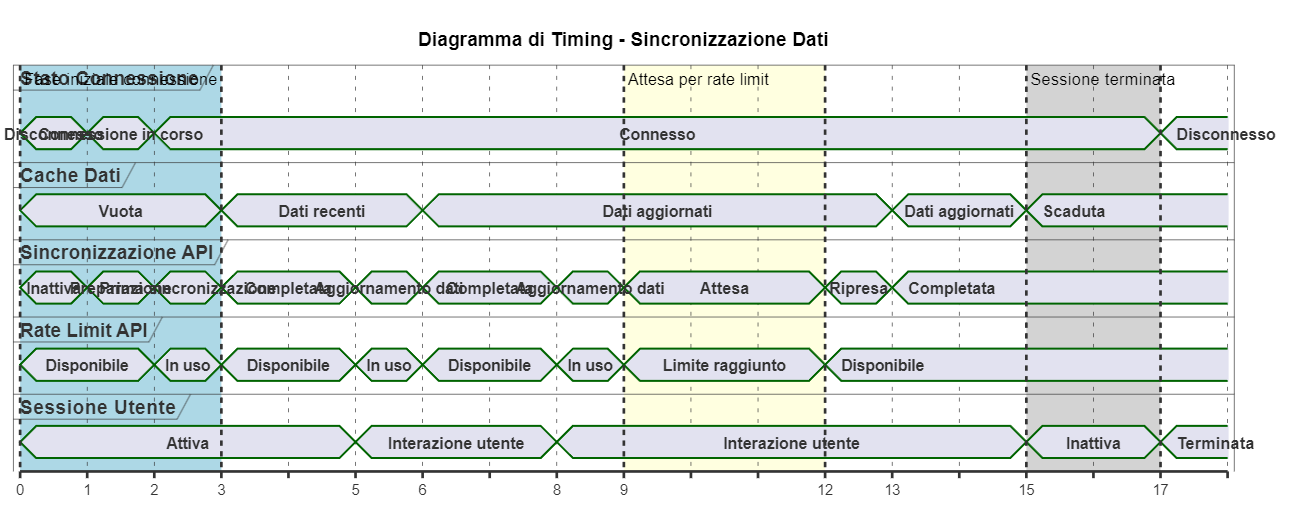
\includegraphics[width=0.85\textwidth]{images/uml/DataSynchronization.png}
    \caption{Grafico UML temporale per la sincronizzazione dei dati}
    \label{fig:uml-temp-graph}
\end{figure}
\begin{lstlisting}[basicstyle=\small\ttfamily, breaklines=true, caption={sincronizzatione dei dati}]
    @startuml "DiagrammaTiming-SincronizzazioneDati"

' Timing diagram for data synchronization
title Diagramma di Timing - Sincronizzazione Dati

concise "Stato Connessione" as Connection
concise "Cache Dati" as Cache
concise "Sincronizzazione API" as Sync
concise "Rate Limit API" as RateLimit
concise "Sessione Utente" as UserSession

@0
Connection is "Disconnesso"
Cache is "Vuota"
Sync is "Inattiva" 
RateLimit is "Disponibile" 
UserSession is "Attiva"

@1
Connection is "Connessione in corso"
Sync is "Preparazione"

@2
Connection is "Connesso"
Sync is "Prima sincronizzazione"
RateLimit is "In uso"

@3
Sync is "Completata"
Cache is "Dati recenti"
RateLimit is "Disponibile"

@5
UserSession is "Interazione utente"
Sync is "Aggiornamento dati"
RateLimit is "In uso"

@6
Sync is "Completata"
Cache is "Dati aggiornati"
RateLimit is "Disponibile"

@8
UserSession is "Interazione utente"
Sync is "Aggiornamento dati"
RateLimit is "In uso"

@9
RateLimit is "Limite raggiunto"
Sync is "Attesa"

@12
RateLimit is "Disponibile" 
Sync is "Ripresa"

@13
Sync is "Completata"
Cache is "Dati aggiornati"

@15
UserSession is "Inattiva"
Cache is "Scaduta"

@17
UserSession is "Terminata"
Connection is "Disconnesso"

highlight 0 to 3 #lightblue : Fase iniziale connessione
highlight 9 to 12 #lightyellow : Attesa per rate limit
highlight 15 to 17 #lightgrey : Sessione terminata

@enduml


\end{lstlisting}

% Bibliografia
\begingroup
\begin{thebibliography}{99}
    \bibitem{msd2025} MSD, Salute. (2025, January 23). \textit{Telemedicina. Ocse: "Raddoppiato il suo uso dopo la pandemia"}. MSD Salute. \url{https://msdsalute.it/approfondimenti/notizie/telemedicina-ocse-raddoppiato-il-suo-uso-dopo-la-pandemia/}
    \bibitem{anastasio2023} Anastasio, P. (2023, February 8). \textit{Sanità digitale, Italia in ritardo. 'Serve collaboration e telemedicina.'}. Key4biz. \url{https://www.key4biz.it/sanita-digitale-italia-ancora-indietro-puntare-su-collaboration-e-telemedicina/434361/}
    \bibitem{validic} \textit{An EHR-integrated solution for remote patient care}. (n.d.). Validic. \url{https://www.validic.com/}
    \bibitem{humanapi} \textit{What is Human API?} (n.d.). Human API. \url{https://reference.humanapi.co/docs/overview}
    \bibitem{withings} \textit{Health Mate by Withings - La migliore app per monitorare la tua attività, peso e altro}. (n.d.). Withings. \url{https://www.withings.com/it/it/health-mate}
    \bibitem{mywellness} SPA, T. (n.d.). \textit{mywellness}. \url{https://www.mywellness.com/cloud/}
    \bibitem{wellmo} Wellmo Mobile Wellness Solutions MWS Oy. (2025, May 6). \textit{Platform and mobile app for personalised digital health services}. Wellmo. \url{https://www.wellmo.com/}
    \bibitem{liva} \textit{Improving lives through digital health coaching | LiVA Healthcare}. (n.d.). \url{https://www.livahealthcare.com/}
    \bibitem{doccla} \textit{Doccla – Europe's leading virtual care solution}. (n.d.). \url{https://www.doccla.com/}
    \bibitem{geeksforgeeks} GeeksforGeeks. (2024, December 10). \textit{Top 7 Backend development Frameworks [2025 Updated]}. GeeksforGeeks. \url{https://www.geeksforgeeks.org/frameworks-for-backend-development/}
    \bibitem{bootstrap} Contributors, M. O. J. T. a. B. (n.d.). \textit{Bootstrap}. \url{https://getbootstrap.com/}
    \bibitem{flutter} \textit{Flutter - Build apps for any screen}. (n.d.) \url{https://flutter.dev/}
    \bibitem{react} \textit{React}. (n.d.). \url{https://react.dev/}
    \bibitem{GDPR} Altalex, R. (2019, February 22). \textit{GDPR - Regolamento generale sulla protezione dei dati}. Altalex. \url{https://www.altalex.com/documents/codici-altlex/2018/03/05/regolamento-generale-sulla-protezione-dei-dati-gdpr}
    \bibitem{mysql} \textit{MySQL}. (n.d.). \url{https://www.mysql.com/it/}
    \bibitem{postgresql} PostgreSQL. (2025, May 7). \textit{PostgreSQL}. \url{https://www.postgresql.org/}
    \bibitem{mongodb} \textit{MongoDB: the world’s leading modern database}. (n.d.). MongoDB. \url{https://www.mongodb.com/}
    \bibitem{bluetooth} \textit{Bluetooth App development: The role of Bluetooth in wearable technology | By Summer Swann | Connected Devices | Yeti LLC}. (n.d.). \url{https://www.yeti.co/blog/bluetooths-role-in-wearable-technology}
    \bibitem{ble} contributori di Wikipedia. (2025, March 21). \textit{Bluetooth Low energy}. Wikipedia. \url{https://it.wikipedia.org/wiki/Bluetooth_Low_Energy}
    \bibitem{ant} contributori di Wikipedia. (2022, March 8). \textit{ANT+}. Wikipedia. \url{https://it.wikipedia.org/wiki/ANT%2B}
    \bibitem{fitbit} contributori di Wikipedia. (2024, April 15). \textit{Fitbit}. Wikipedia. \url{https://it.wikipedia.org/wiki/Fitbit}
    \bibitem{fitbitapi} \textit{Fitbit Development: Intraday}. (n.d.). \url{https://dev.fitbit.com/build/reference/web-api/intraday/}
    \bibitem{garmin} \textit{Smartwatch | Orologi per lo Sport | GARMIN}. (n.d.). \url{https://www.garmin.com/it-IT/c/wearables-smartwatches/}
    \bibitem{applewatch} Apple. (n.d.). \textit{Apple Watch}. Apple (Italia). \url{https://www.apple.com/it/watch/}
    \bibitem{amazfit} amazfit-it. (2025, April 30). \textit{Amazfit Italia | Negozio online ufficiale}. Amazfit-it. \url{https://it.amazfit.com/}
    \bibitem{moscow} contributori di Wikipedia. (2024, September 5). \textit{Metodo MOSCOW}. Wikipedia. \url{https://it.wikipedia.org/wiki/Metodo_MoSCoW}
    \bibitem{werkzeug} \textit{Werkzeug — Werkzeug Documentation (3.1.x)}. (n.d.). \url{https://werkzeug.palletsprojects.com/en/stable/}
    \bibitem{oauth-image} Google Cloud. (n.d.). \textit{Flusso di autorizzazione OAuth 2.0}. Google Cloud Apigee. \url{https://cloud.google.com/static/apigee/docs/api-platform/images/oauth-abstract.png}
    \bibitem{sqlalchemy} SQLAlchemy. (n.d.). \url{https://www.sqlalchemy.org/}
    \bibitem{chartjs} Chart.js. (n.d.). Open Source HTML5 Charts for Your Website. \url{https://www.chartjs.org/}
    \bibitem{rest} contributori di Wikipedia. (2025, March 15). Representational state transfer. Wikipedia. \url{https://it.wikipedia.org/wiki/Representational_state_transfer}
    \bibitem{json} JSON. (n.d.). \url{https://www.json.org/json-it.html}
    \bibitem{orm} Admin. (2024, February 25). Cosa è un ORM. Innovaformazione - Informatica Specialistica. \url{https://innovaformazione.net/cosa-e-un-orm/}
    \bibitem{github} andrearoggeri22/VitaLink: Piattaforma di monitoraggio dati vitali per pazienti in contesto di analisi e valutazione di terapie. (n.d.). GitHub. \url{https://github.com/andrearoggeri22/VitaLink}
    \bibitem{gitdesktop} Download GitHub Desktop. (n.d.). GitHub Desktop. \url{https://desktop.github.com/download/}
    \bibitem{code-docs} Roggeri, A. (n.d.). VitaLink Documentation. \url{https://andrearoggeri22.github.io/VitaLink/code/}
    \bibitem{tests-docs} Roggeri, A. (n.d.). VitaLink Documentation. \url{https://andrearoggeri22.github.io/VitaLink/tests/}
    \bibitem{analysis-docs} Static Analysis report. (n.d.). \url{https://andrearoggeri22.github.io/VitaLink/analysis/}
    \bibitem{plantuml} PlantUML. (n.d.). Open-source tool that uses simple textual descriptions to draw beautiful UML diagrams. PlantUML.com. \url{https://plantuml.com/}
    \bibitem{plantvscode} PlantUML - Visual Studio Marketplace. (n.d.). \url{https://marketplace.visualstudio.com/items?itemName=jebbs.plantuml}
    \bibitem{pytest} pytest documentation. (n.d.). \url{https://docs.pytest.org/en/stable/}
    \bibitem{koyeb} KOYEB: High-performance infrastructure for APIs, inference, and databases. (n.d.). Koyeb. \url{https://www.koyeb.com/}
    \bibitem{fitbit_API_rate} Fitbit API - PublicAPI. (n.d.). PublicAPI. \url{https://publicapi.dev/fitbit-api}
  \end{thebibliography}
\end{document}